\documentclass{ConfigurationFiles/PoliMi3i_Thesis}


% CONFIGURATIONS
\usepackage{parskip} % For paragraph layout
\usepackage{setspace} % For using single or double spacing
\usepackage{emptypage} % To insert empty pages
\usepackage{multicol} % To write in multiple columns (executive summary)
\setlength\columnsep{15pt} % Column separation in executive summary
\setlength\parindent{0pt} % Indentation
\raggedbottom
\usepackage{multirow}

% PACKAGES FOR TITLES
\usepackage{titlesec}
% \titlespacing{\section}{left spacing}{before spacing}{after spacing}
\titlespacing{\section}{0pt}{3.3ex}{2ex}
\titlespacing{\subsection}{0pt}{3.3ex}{1.65ex}
\titlespacing{\subsubsection}{0pt}{3.3ex}{1ex}
\usepackage{color}

% PACKAGES FOR LANGUAGE AND FONT
\usepackage[english]{babel} % The document is in English  
\usepackage[utf8]{inputenc} % UTF8 encoding
\usepackage[T1]{fontenc} % Font encoding
\usepackage[11pt]{moresize} % Big fonts

% PACKAGES FOR IMAGES
\usepackage{graphicx}
\usepackage{transparent} % Enables transparent images
\usepackage{eso-pic} % For the background picture on the title page
\usepackage{subfig} % Numbered and caption subfigures using \subfloat.
\usepackage{tikz} % A package for high-quality hand-made figures.
\usetikzlibrary{}
\graphicspath{{./Images/}} % Directory of the images
\usepackage{amsthm} % Coloured "Theorem"
\usepackage{thmtools}
\usepackage{xcolor}
\usepackage{float}

% STANDARD MATH PACKAGES
\usepackage{amsmath}
\usepackage{amssymb}
\usepackage{amsfonts}
\usepackage{bm}
\usepackage[overload]{empheq} % For braced-style systems of equations.
\usepackage{fix-cm} % To override original LaTeX restrictions on sizes

% PACKAGES FOR TABLES
\usepackage{tabularx}
\usepackage{longtable} % Tables that can span several pages
\usepackage{colortbl}

% PACKAGES FOR ALGORITHMS (PSEUDO-CODE)
\usepackage{algorithm}
\usepackage{algorithmic}


% PACKAGES FOR REFERENCES & BIBLIOGRAPHY
\usepackage[
    colorlinks=true,
    linkcolor=black,
    anchorcolor=black,
    citecolor=black,
    filecolor=black,
    menucolor=black,
    runcolor=black,
    urlcolor=black
]{hyperref} % Adds clickable links at references
\usepackage{cleveref}
\usepackage[square, numbers, sort&compress]{natbib} % Square brackets, citing references with numbers, citations sorted by appearance in the text and compressed
\bibliographystyle{abbrvnat} % You may use a different style adapted to your field

% OTHER PACKAGES
\usepackage{pdfpages} % To include a pdf file
\usepackage{afterpage}
\usepackage{lipsum} % DUMMY PACKAGE
\usepackage{fancyhdr}
\usepackage{wasysym} % For the headers
\usepackage{rotating}
\usepackage{listings}
\usepackage{csquotes}
\fancyhf{}

% Input of configuration file. Do not change config.tex file unless you really know what you are doing. 
% Define blue color typical of polimi
\definecolor{bluepoli}{cmyk}{0.4,0.1,0,0.4}

% Custom theorem environments
\declaretheoremstyle[
    headfont=\color{bluepoli}\normalfont\bfseries,
    bodyfont=\color{black}\normalfont\itshape,
]{colored}

% Set-up caption colors
\captionsetup[figure]{labelfont={color=bluepoli}} % Set colour of the captions
\captionsetup[table]{labelfont={color=bluepoli}} % Set colour of the captions
\captionsetup[algorithm]{labelfont={color=bluepoli}} % Set colour of the captions

\theoremstyle{colored}
\newtheorem{theorem}{Theorem}[chapter]
\newtheorem{proposition}{Proposition}[chapter]

% Enhances the features of the standard "table" and "tabular" environments.
\newcommand\T{\rule{0pt}{2.6ex}}
\newcommand\B{\rule[-1.2ex]{0pt}{0pt}}

% Pseudo-code algorithm descriptions.
\newcounter{algsubstate}
\renewcommand{\thealgsubstate}{\alph{algsubstate}}
\newenvironment{algsubstates}
{\setcounter{algsubstate}{0}%
\renewcommand{\STATE}{%
    \stepcounter{algsubstate}%
    \Statex {\small\thealgsubstate:}\space}}
{}

% New font size
\newcommand\numfontsize{\@setfontsize\Huge{200}{60}}

% Title format: chapter
\titleformat{\chapter}[hang]{
    \fontsize{50}{20}\selectfont\bfseries\filright}{\textcolor{bluepoli} \thechapter\hsp\hspace{2mm}\textcolor{bluepoli}{|   }\hsp}{0pt}{\huge\bfseries \textcolor{bluepoli}
}

% Title format: section
\titleformat{\section}
{\color{bluepoli}\normalfont\Large\bfseries}
{\color{bluepoli}\thesection.}{1em}{}

% Title format: subsection
\titleformat{\subsection}
{\color{bluepoli}\normalfont\large\bfseries}
{\color{bluepoli}\thesubsection.}{1em}{}

% Title format: subsubsection
\titleformat{\subsubsection}
{\color{bluepoli}\normalfont\large\bfseries}
{\color{bluepoli}\thesubsubsection.}{1em}{}

% Shortening for setting no horizontal-spacing
\newcommand{\hsp}{\hspace{0pt}}

\makeatletter
% Renewcommand: cleardoublepage including the background pic
\renewcommand*\cleardoublepage{%
    \clearpage\if@twoside\ifodd\c@page\else
    \null
    \AddToShipoutPicture*{\BackgroundPic}
    \thispagestyle{empty}%
    \newpage
    \if@twocolumn\hbox{}\newpage\fi\fi\fi}
\makeatother

%For correctly numbering algorithms
\numberwithin{algorithm}{chapter}



\definecolor{dkgreen}{rgb}{0,0.6,0}
\definecolor{gray}{rgb}{0.5,0.5,0.5}
\definecolor{mauve}{rgb}{0.58,0,0.82}


\newcommand{\ckbautoref}[1] {%
	\hypersetup{linkcolor=gray}%
	\autoref{#1}%
}



%----------------------------------------------------------------------------
%	BEGIN OF YOUR DOCUMENT
%----------------------------------------------------------------------------



\begin{document}
    \fancypagestyle{plain}{%
        \fancyhf{} % Clear all header and footer fields
        \fancyhead[RO,RE]{\thepage} %RO=right odd, RE=right even
        \renewcommand{\headrulewidth}{0pt}
        \renewcommand{\footrulewidth}{0pt}}

        
    \pagestyle{empty} % No page numbers
    \frontmatter % Use roman page numbering style (i, ii, iii, iv...) for the preamble pages

    \puttitle{
        title=Software Engineering 2\\Design Document,
        name1=Pica Mirko - 10811404, % Author Name and Surname
        name2=Pianalto Riccardo - 10835980,
        name3=Prendin Christian - 10827556,
        academicyear=2024-2025,
        version=1.0,
        releasedate=07/01/2025,
          }
    
    
    \startpreamble
    \setcounter{page}{1} % Set page counter to 1


% TABLE OF CONTENTS
    \thispagestyle{empty}
    \tableofcontents % Table of contents
    \thispagestyle{empty}
    \cleardoublepage

    
    \addtocontents{toc}{\vspace{2em}} % Add a gap in the Contents, for aesthetics
    \mainmatter % Begin numeric (1,2,3...) page numbering


    \chapter{Introduction}
    \label{ch:introduction}%
    \section{Purpose}
\label{sec:purpose}%
The purpose of this document is to present a detailed description of Students\&Company.
It is addressed to the developers who have to implement the requirements and could be used as an agreement between the customer and the contractors.\\ 
The document is also intended to provide the customer with a clear and unambiguous description of the system's functionalities and constraints, allowing the customer to validate the requirements and to verify if the system meets the expectations.

\section{Scope}
\label{sec:scope}%
Students\&Companies (S\&C) is a platform designed to simplify and optimize the matching process between university students looking for internship opportunities and companies offering them. The system analyzes students' profiles, CVs, and indicated preferences, relating them to internship offers posted by companies, which include details on required skills, technologies used, and proposed conditions. Using sophisticated recommendation algorithms, S\&C suggests suitable opportunities to students and notifies companies of candidates who best meet their needs. The platform also supports the entire selection cycle, from application and interview management to feedback collection, ensuring a structured and transparent experience for all users involved, including universities that monitor the progress of internships and resolve any issues.



\section{Definition, Acronyms, Abbreviations}
\label{sec:definition_acronyms_abbreviations}%

\begin{table}[H]
    \begin{center}
        \begin{tabular}{ |l|l| }
            \hline
            \textbf{Acronyms} & \textbf{Definition}                              \\
            \hline
            DD             & Design Document                      \\
            \hline            
            RASD             & Requirements Analysis \& Specification Document     \\   
            \hline
            ST              & Student                         \\
            \hline
            ED              & Educator                         \\
            \hline
            STG             & Student Group                    \\
            \hline
            CKB             & CodeKataBattle                   \\
            \hline
            GH              & GitHub                           \\
            \hline
            User            & All STs and EDs                           \\
            \hline
            API             & Application Programming Interface       \\
            \hline
            RX              & Requirement X                           \\
            \hline
            CMP            & Component                           \\
            \hline
         \end{tabular}
        \caption{Acronyms used in the document.}
        \label{tab:acronyms}%
    \end{center}
\end{table}

\section{Revision History}
\label{sec:revision_history}%
\textbf{Version 1.0} - 07/01/2024

\section{Reference Documents}
\label{sec:reference_documents}%

\begin{itemize}
    \item Specification Document Assignment
\end{itemize}

\section{Document Structure}
\label{sec:doc_structure}%
The document is structured in seven sections, as described below.

\textbf{Introduction}. In the first section, the chapter elucidates the significance of the Design 
Document, providing comprehensive definitions and explanations of acronyms and abbreviations. Additionally, it recalled the scope of the CodeKateBattle system.

\textbf{Architectural Design}. The second section shows the main components of the system and their relationships. This section also focuses on design choices and architectural styles, patterns and paradigms.

\textbf{User Interface Design}. The next section, the third, describes the user interface of the system, providing mockups and explanations of the main pages.

\textbf{Requirements Traceability}. The fourth section describes the requirements of the system, showing how they are satisfied by the design choices.

\textbf{Implementation, Integration and test Plan}. This fifth part provides an overview of the implementation of the various components of the system, it also shows how they are integrated and it gives a plan for testing them all.

\textbf{Effort Spent}. In the sixth section are included information about the number of hours each group member has worked for this document.

\textbf{References}. The last section contains the list of the documents used to redact this Design Document.
 



    \chapter{Architectural Design}
    \label{ch:rchitectural_design}%
    \section{Overview}
\label{sec:overview}%
Here we represent an overview of how the entire S\&C architecture is composed of:

\begin{figure}[H]
    \begin{center}
        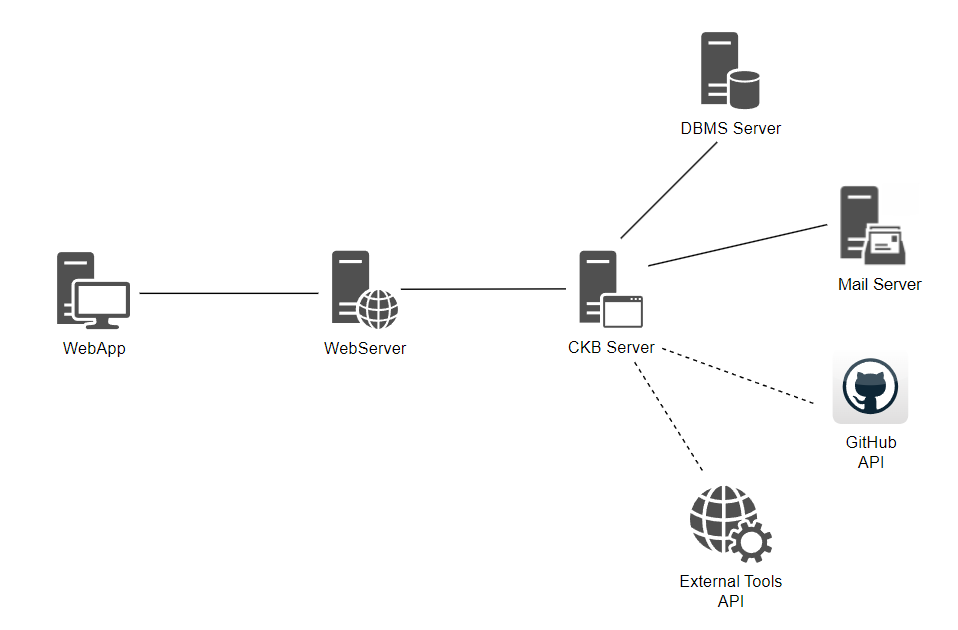
\includegraphics[width=1\linewidth]{CD_DD/Overview.png}
        \caption{S\&C Overview.}
        \label{fig:CKB_overview}%
    \end{center}
\end{figure}

\noindent Client side:
\begin{itemize}
    \item WebApp: serves as the User interface, allowing all Users to connect to CKB. It enables Users to perform operations such as registration, login, creating or joining Tournaments and Battles, creating or modifying Badges and searching for other Users.
\end{itemize}
\noindent Server side:
\begin{itemize}
    \item \textbf{Web Server:} handles communication with Users, receiving and processing their inputs. Additionally, it provides load balancing for requests, distributing them among various replicas of the CKB Server. It also manages the User sessions.
    \item \textbf{CKB Server:} is the central component where interfaces are located, facilitating communication between the Web Server and databases/APIs. It serves as the primary server for the entire website and is replicated across multiple machines to handle a high volume of requests.
    \item \textbf{DBMS Server:} stores data related to Users, Tournaments, Group, Badges and Battles. It acts as the repository for essential information.
    \item \textbf{Mail Server:} is responsible for sending confirmation eMails when a new User registers on CKB, enhancing the User registration process.
    \item \textbf{GitHub API:} is utilized for communication with GitHub, facilitating the creation of the Battle repository and allowing STGs to fork the repository to push their code.
    \item \textbf{External Tools API:} used to automatically test the STG code when a new push is made. It is also used to retrieve the results of the tests and update the Battle dashboard.
\end{itemize}

\section{Component View}
\label{sec:component_view}%

\subsection{High Level Diagram}
\label{subsec:high_level_diagram}%

\begin{figure}[H]
    \begin{center}
        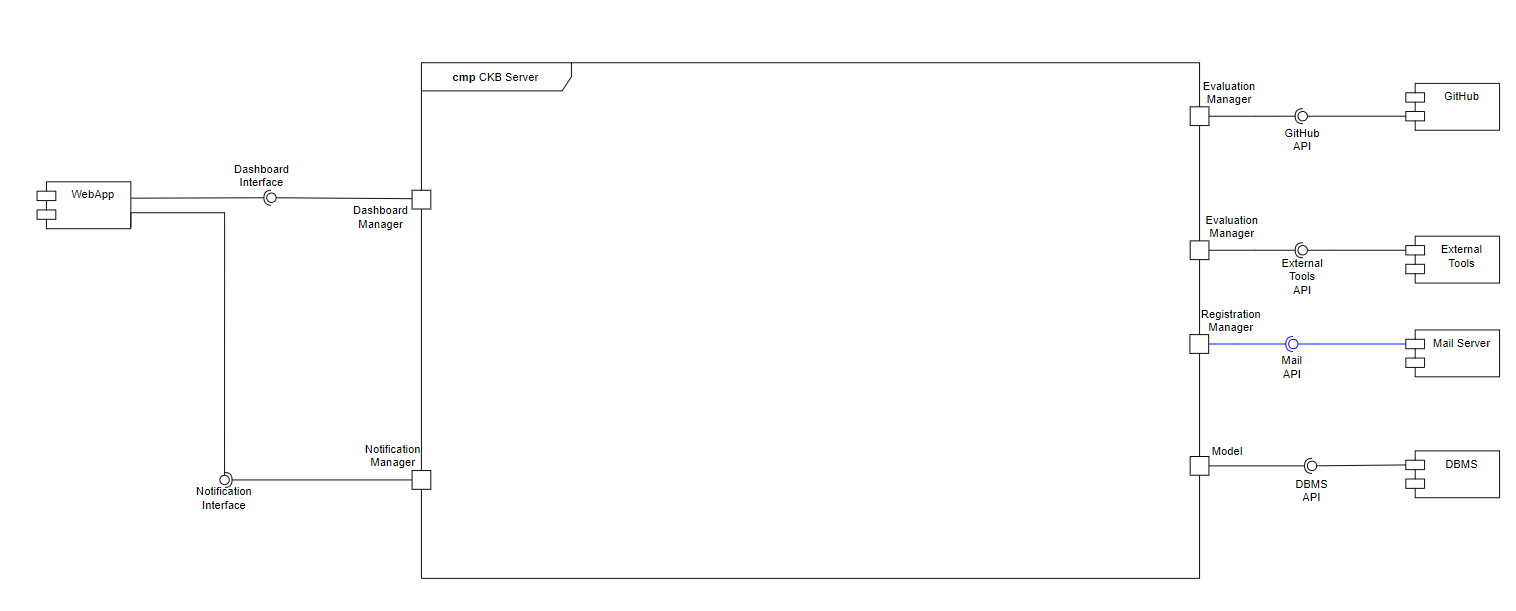
\includegraphics[width=1\linewidth]{CD_DD/HighLevel.png}
        \caption{High Level Diagram.}
        \label{fig:high_level_diagram}%
    \end{center}
\end{figure}

\noindent In the figure above is the high level component diagram of CKB where it’s represented the external components of CKB and how they communicate with the CKB server, in particular:
\begin{itemize}
    \item \textbf{WebApp}: serves as the external access point for Users, allowing communication with the CKB Server through the Dashboard Interface—the sole means for Client-Server interaction from the User side. The CKB Server can relay notifications, such as Tournament or Battle creation, to Users through the Notification Interface.
    \item \textbf{DBMS:} is the storage repository for all User, Tournament, and Battle data. It communicates with the CKB Server via the DBMS API, which is connected to the Model component.
    \item \textbf{Mail Server:} responsible for sending registration confirmation eMails, the Mail Server communicates with the CKB Server using the Mail API interface. This interface is linked to the Registration Manager component, which oversees the User registration process..
    \item \textbf{External Tools:} external application used for testing the code submitted by STGs on GitHub. It communicates with the CKB Server through the External Tools API, connecting to the Evaluation Manager component. The Evaluation Manager handles the evaluation process for STG-submitted code.
    \item \textbf{GitHub:}  external website used to create repositories for the code katas of Battles. Each STG, after forking the main repository, pushes their code for evaluation. GitHub communicates with the CKB Server through the GitHub API, linked to the Evaluation Manager.
\end{itemize}

\subsection{Low Level Diagram}
\label{subsec:low_level_diagram}%

\begin{figure}[H]
    \begin{center}
        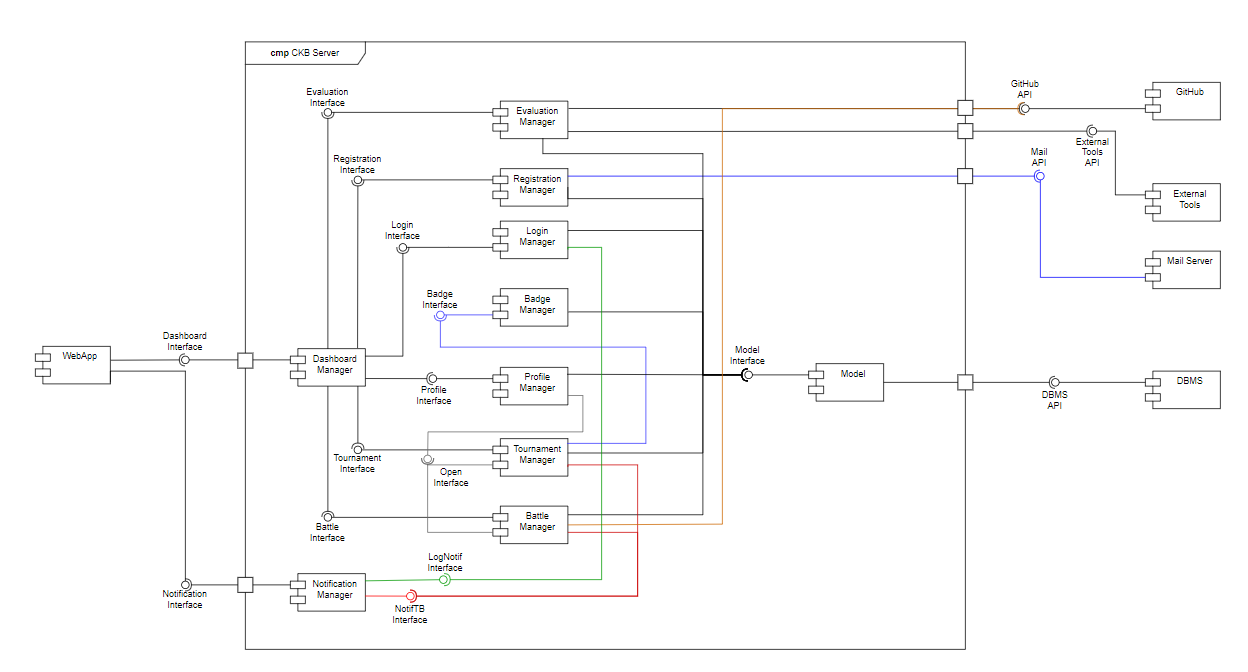
\includegraphics[width=1\linewidth]{CD_DD/LowLevel.png}
        \caption{Low Level Diagram.}
        \label{fig:low_level_diagram}%
    \end{center}
\end{figure}

\noindent The figure above represents the complete architecture of CKB website with each components inside the CKB Server:
\begin{itemize}
    \item \textbf{Dashboard Manager:} pivotal component that orchestrates all communication between Users and the CKB website. Users interact with CKB through the Dashboard Interface, and the Dashboard Manager directs requests to the appropriate components. It serves as the central hub for user interactions.
    \item \textbf{Model:} This high-level component represents the data on the server and acts as an interface to the database server. It acts as a mask to the database server, and every component needs to interface with it to access data from the DBMS through the DBMS API.
    \item \textbf{Evaluation Manager:} component that handles the code evaluation both when a new push is made by a STG on GH or when an ED wants to manually evaluate a STG code during the consolidation stage of a Battle, more detailed information in \ckbautoref{fig:evaluation_manager}. This component communicates with the Dashboard manager through the Evaluation Interface, with the Model component through the Model Interface to add and modify the STG evaluation in the DBMS, with GitHub through the GitHub API when a new push is made by a STG and with the External Tools through the External Tools API to automatically evaluate a STG code.
    \item \textbf{Registration Manager:} component that handles the registration of a new User. When a new User wants to create an account on CKB system he communicates with the Dashboard Manager that forwards the request to the Registration Manager through the registration interface. Then the Registration Manager handles the request and communicates through the Mail API to the Mail Server, to send a confirmation mail to the new User, and through the Model Interface to the Model component to add the new User’s information to the DBMS. This component also gives the permission to the User that registered as an Educator to create Tournaments, Battles and Badges.
    \item \textbf{Login Manager:} component that handles the login process for registered Users. When a User attempts to log in, the Dashboard Manager forwards the request to the Login Manager through the Login Interface. The Login Manager communicates with the Model component through the Model interface to retrieve the User's data from the DBMS.
    \item \textbf{Badge Manager:} component that handles the Badges creation and modification when a new Tournament is created. When the ED creates a new Tournament, the Badge Manager component receives a request from the Tournament Manager through the Badge Interface and lets the ED create new Badges or modify existing ones, more details in \ckbautoref{fig:badge_manager}. The new Badges are added in the DBMS through the communication between the Badge Manager and the Model component through the Model Interface.
    \item \textbf{Profile Manager:} component that allows User profile search and profile open in both Tournament and Battle dashboard. When a User initiates a search, the Dashboard Manager forwards the request to the Profile Manager using the Profile Interface. The Profile Manager communicates with the Model component through the Model Interface to retrieve relevant information from the DBMS.This component also manages the open profile operation within a Tournament or Battle dashboard, more detail in \ckbautoref{fig:profile_manager}.
    \item \textbf{Tournament Manager:} component that manages all Users' actions related to Tournaments; more detailed information in \ckbautoref{fig:tournament_manager}. It communicates with the Dashboard Manager through the Tournament Interface, with the Notification Manager through the NotifTB Interface when a new Tournament is created or closed and with the Model component through the Model Interface to add or retrieve data from the DBMS.
    \item \textbf{Battle Manager:} component that manages all Users' actions related to Battles; more detailed information in \ckbautoref{fig:battle_manager}. It communicates with the Dashboard Manager through the Battle iIterface, with the Notification Manager through the NotifTB Interface when a new Battle is created or when a ST invites other STs to join his STG and with the Model component through the Model Interface to add or retrieve data from the DBMS. It also communicates with GitHub through the GitHub API to create repositories and upload code katas for new Battles.
    \item \textbf{Notification Manager:} component that handles each notification that has to be sent to the Users in particular when a new Tournament is created it sends a notification to all STs registered in CKB, when a new Battle is created it sends a notification to all the STs that have joined that specific Tournament, when a ST invites another ST to join his STG for a battle a notification is sent to the second ST and when a Tournaments is closed and the score are updated it sends a notification to all the STs that have joined the Tournament. All the communication from the Battle Manager and the Tournament Manager with the Notification Manager is made through the NotifTB Interface and the communication with the WebApp is made through the Notification Interface.
\end{itemize}

\subsection{Evaluation Manager}
\label{subsec:evaluation_manager}%

\begin{figure}[H]
    \begin{center}
        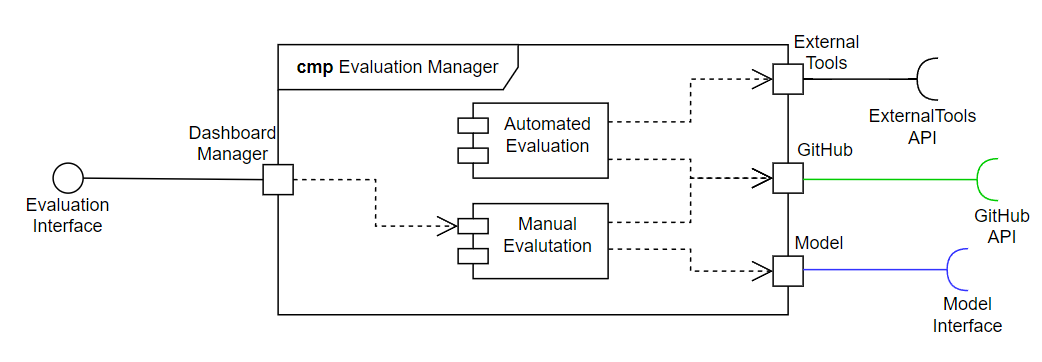
\includegraphics[width=1\linewidth]{CD_DD/Evaluation Manager.png}
        \caption{Evaluation Manager.}
        \label{fig:evaluation_manager}%
    \end{center}
\end{figure}

\noindent The Evaluation Manager is composed by two other sub-components that handles the two different evaluation method of a STG code:

\begin{itemize}
    \item \textbf{Automated Evaluation component:} utilized by the CKB system to automatically evaluate STG code whenever a new push is made to the STG's forked repository on GitHub. When a code update occurs, GitHub communicates with the Automated Evaluation component through the GitHub API. Subsequently, the Automated Evaluation component sends the code to External Tools via the External Tools API, where the code undergoes testing and evaluation. Upon receiving the evaluation results, the Automated Evaluation component, through the Model interface, communicates with the Model component. The Model component utilizes the DBMS API to update the new score in the relevant DBMS section associated with the corresponding Battle.
    \item \textbf{Manual Evaluation component:} comes into play when an ED wishes to manually assess an STG code. The process begins with the WebApp, which, through the Dashboard Interface, requests the STG code from the Dashboard Manager. The Dashboard Manager then communicates this request to the Manual Evaluation component through the Evaluation Interface. Subsequently, the Manual Evaluation component communicates with the GitHub API to retrieve the source code from the STG's forked repository, allowing the ED to analyze it. Once the evaluation is complete and the ED decides to update the score, the Manual Evaluation component, through the Model Interface, communicates with the Model component. The Model component, utilizing the DBMS API, updates the score in the DBMS, ensuring the manual evaluation results are recorded appropriately.
\end{itemize}

\subsection{Badge Manager}
\label{subsec:badge_manager}%

\begin{figure}[H]
    \begin{center}
        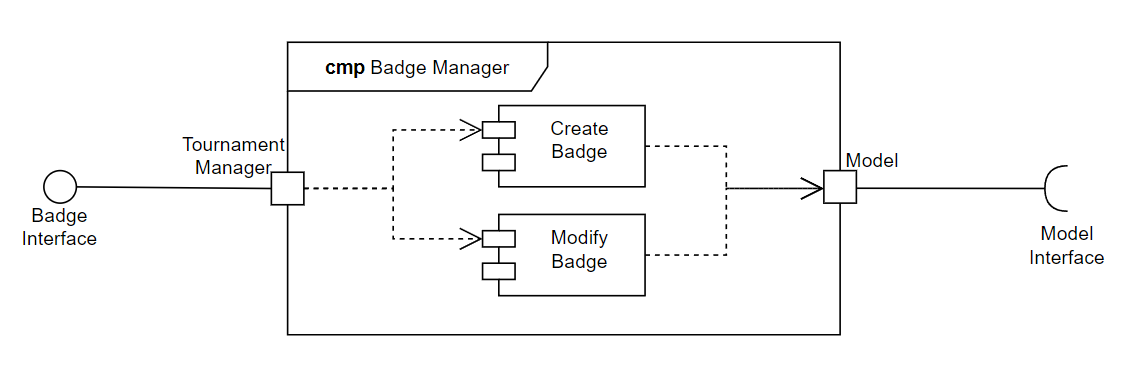
\includegraphics[width=1\linewidth]{CD_DD/Badge Manager.png}
        \caption{Badge Manager.}
        \label{fig:badge_manager}%
    \end{center}
\end{figure}

\noindent The Badge Manager is the component used by the CKB system to handle the creation and the modification of the Badges during the Tournament creation:

\begin{itemize}
    \item \textbf{Create Badge component:} activated when an ED intends to create a new Badge for a newly created Tournament. The initiation of this process is through the Create Tournament component, a sub-component of the Tournament Manager. The Create Tournament component, via the Badge Interface, sends a request to the Create Badge component, allowing the ED to define the Badge with its specific settings and parameters, such as the criteria STs must fulfill to obtain it. Following the Badge creation, the Create Badge component, through the Model Interface, communicates with the Model component, ensuring the newly created Badge is added to the DBMS.
    \item \textbf{Modify Badge component:} engaged when an ED aims to modify an existing Badge that was previously created for another Tournament. The process is initiated by the Create Tournament component, a sub-component of the Tournament Manager. The Create Tournament component, via the Badge Interface, sends a request to the Modify Badge component, allowing the ED to adjust parameters associated with an existing Badge, specifying new criteria for STs to fulfill. Once the Badge is successfully modified, the Modify Badge component, through the Model Interface, communicates with the Model component. This communication ensures that the updated Badge information is reflected in the DBMS.
\end{itemize}

\subsection{Profile Manager}
\label{subsec:profile_manager}%

\begin{figure}[H]
    \begin{center}
        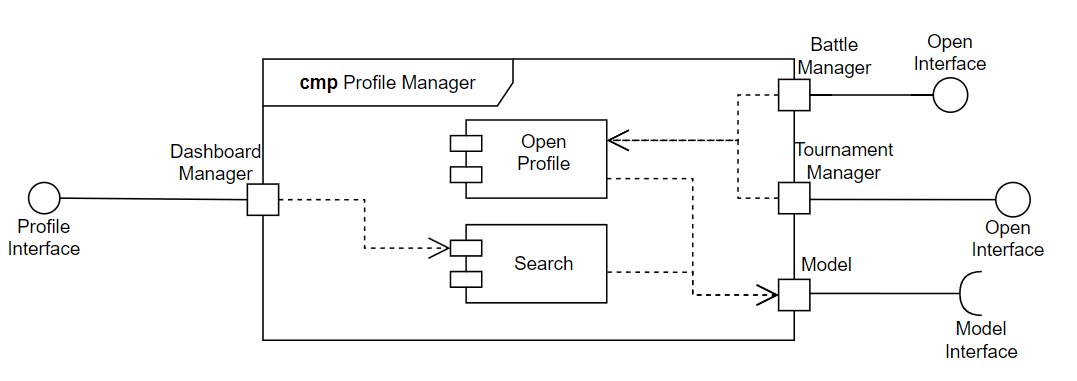
\includegraphics[width=1\linewidth]{CD_DD/Profile Manager.png}
        \caption{Profile Manager.}
        \label{fig:profile_manager}%
    \end{center}
\end{figure}

\noindent The Profile Manager is the component used by the CKB system to handle the research of a User’s profile and the visualization of another User’s profile when the User clicks on a nickname within the Tournament or Battle dashboard:

\begin{itemize}
    \item \textbf{Search component:} responsible for managing the profile search process when a User enters a nickname or keyword into the search bar across various CKB pages. When a User initiates a search by entering another User's nickname or a relevant keyword, the Dashboard Manager communicates with the Search component through the Profile Interface. The Search component then forwards the search request to the Model component via the Model Interface. Subsequently, the Model component retrieves the profile information from the DBMS. The retrieved information is then presented to the User, allowing him to visualize the searched User's profile.
    \item \textbf{Open Profile component:} manages the retrieval of a User's profile when a User clicks on a nickname within a Tournament or Battle dashboard. When a User clicks on another User's nickname in a Tournament or Battle dashboard, the Dashboard Manager communicates with the View component within the Tournament or Battle Manager. The View component forwards the request to the Open Profile component through the Open Interface. The Open Profile component communicates with the Model component via the Model Interface. This communication with the Model component facilitates the retrieval of the User's profile information from the DBMS. The retrieved profile information is then presented to the User, allowing them to view the selected User's profile.
\end{itemize}

\subsection{Tournament Manager}
\label{subsec:tournament_manager}%

\begin{figure}[H]
    \begin{center}
        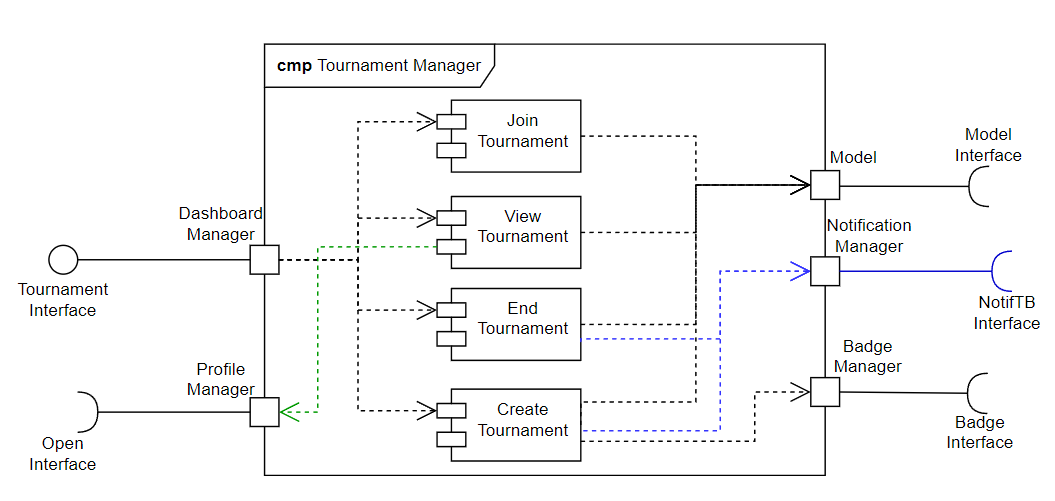
\includegraphics[width=1\linewidth]{CD_DD/Tournament Manager.png}
        \caption{Tournament Manager.}
        \label{fig:tournament_manager}%
    \end{center}
\end{figure}

\noindent The Tournament Manager is the component used by the CKB system to handle every aspect of the Tournament, from the creation to the end going through the Join and the View sub-components:

\begin{itemize}
    \item \textbf{Create Tournament component:} utilized when an ED initiates the creation of a new Tournament. The ED communicates with the Dashboard Manager through the Dashboard Interface, which then directs the request to the Create Tournament component. This component sends back a creation form for the ED to fill. Once completed, the Create Tournament component communicates the data to the Model component through the Model Interface, adding the information to the DBMS via the DBMS API. If the ED grants permissions to other EDs, the Create Tournament component communicates with the Notification Manager through the NotifTB Interface to notify the specified EDs. Additionally, notifications are sent to all the STs via the Notification Manager, informing them of the new Tournament. Throughout the Tournament creation process, the Create Tournament component also communicates with the Badge Manager through the Badge Interface, allowing the ED to create or modify Badges associated with the Tournament.
    \item \textbf{Join Tournament component:} activated when an ST wishes to join a Tournament. The ST communicates with the Dashboard Manager through the Dashboard Interface, and the request is forwarded to the Join Tournament component. This component communicates through the Model Interface with the Model component to add the ST to the Tournament participant list in the DBMS through the DBMS API. 
    \item \textbf{View Tournament component:} used by the CKB system to let the User visualize the Tournament page with all the information, like the available Battles and the Dashboard with the STs score. When a User wants to search a Tournament it writes the Tournament name or a keyword in the search bar and it communicates with the Dashboard Manager through the Dashboard Interface that forwards the request to the View Tournament component that communicates with the Model component through the Model Interface to retrieve all the information from the DBMS through the DBMS API and let the User visualize the Tournament page. The same communication is made when a User clicks on a Tournament name in another User’s profile or in his main dashboard page. This component also manages the open profile operation when a User wants to visualize another User’s profile from the Tournament dashboard; when a User clicks on another User’s nickname in the Tournament dashboard the Dashboard Manager communicates through the Dashboard Interface with the View Tournament component that forwards the request to the the Profile Manager through the Open Interface.
    \item \textbf{End Tournament component:} triggered when an ED decides to close a Tournament, preventing further ST participation and ED creation of Battles within it. The ED communicates with the Dashboard Manager through the Dashboard Interface, which forwards the request to the Close Tournament component. The Close Tournament component communicates with the Model component through the Model Interface, modifying the Tournament's status to make it non-joinable in the DBMS through the DBMS API. Additionally, the Close Tournament component communicates through the NotifTB Interface to the Notification Manager, which sends notifications to all STs who participated in the Tournament, informing them that final scores are ready for viewing.
\end{itemize}

\subsection{Battle Manager}
\label{subsec:battle_manager}%

\begin{figure}[H]
    \begin{center}
        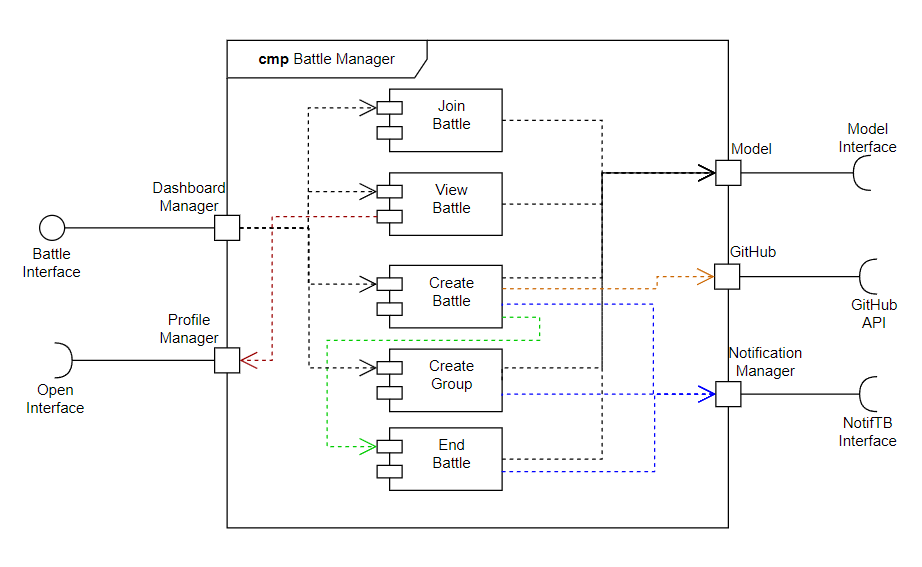
\includegraphics[width=1\linewidth]{CD_DD/Battle Manager.png}
        \caption{Battle Manager.}
        \label{fig:battle_manager}%
    \end{center}
\end{figure}

\noindent The Battle Manager is the component used by the CKB system to handle every aspect of the Battle, from the creation to the end going through the Join, the View and the Create Group sub-components:

\begin{itemize}
    \item \textbf{Create Battle component:} engaged when an ED wishes to create a new Battle within a Tournament. The ED communicates with the Dashboard Manager through the Dashboard Interface, forwarding the request to the Create Battle component. The Create Battle component responds by sending a creation form to be filled by the ED. Upon completion, the component communicates the data to the Model component through the Model Interface, adding the information to the DBMS through the DBMS API. Additionally, the Create Battle component communicates with the Notification Manager through the NotifTB Interface, notifying all STs who have joined the relevant Tournament about the new Battle. It also collaborates with the End Battle component to create a timer, ensuring that after the consolidation stage concludes, the End Tournament component notifies all STs about the availability of final grades. The Create Battle component also communicates with GitHub through the GitHub API to create a new repository and upload the code kata for the Battle. This repository is later forked by all STGs to submit their code.
    \item \textbf{Join Battle component:} activated when an ST intends to join a Battle. The ST communicates with the Dashboard Manager through the Dashboard Interface, and the request is forwarded to the Join Battle component. The Join Battle component, through the Model Interface, communicates with the Model component, adding the ST to the participant list of the Battle in the DBMS through the DBMS API.
    \item \textbf{View Battle component:} used by the CKB system to let the User visualize the Battle page with the dashboard including all the STGs score. When a User wants to visualize the Battle page it communicates with the Dashboard Manager through the Dashboard Interface that forwards the request to the View Battle component that communicates with the Model component through the Model Interface to retrieve all the information from the DBMS through the DBMS API and finally let the User visualize the Battle page. This component also manages the open profile operation when a User wants to visualize another User’s profile from the Battle dashboard; when a User clicks on another User’s nickname in the Battle dashboard the Dashboard Manager communicates through the Dashboard Interface with the View Tournament component that forwards the request to the the Profile Manager through the Open Interface.
    \item \textbf{Create Group component} engaged when STs want to create a new STG for a Battle. After joining a Battle before the registration deadline expires, an ST can create an STG to participate in the battle. The ST communicates with the Dashboard Manager through the Dashboard Interface, initiating a request to create a new STG. The request is forwarded to the Create Group component through the Battle Interface, allowing the ST to decide the STG name and invite other STs. Notifications are sent through the Notification Manager, which communicates with the Battle Manager through the NotifTB interface and with the WebApp through the Notification Interface. When the STG is confirmed, the Create Group component communicates through the Model Interface with the Model component to add the newly created STG to the DBMS through the DBMS API.
    \item \textbf{End Battle component:} activated to notify all STGs that the final scores of the Battle are available. When the consolidation stage concludes, and the timer created by the Create Battle component expires, the End Battle component communicates through the Model Interface with the Model component, updating the scores in the DBMS through the DBMS API. It also notifies all participating STs through the Notification Manager, communicating through the NotifTB Interface, that the final scores are accessible on the Battle page. Communication between the Notification Manager and the WebApp is facilitated through the Notification Interface.
\end{itemize}


\section{Deployment View}
\label{sec:deployment_view}%

In this section it will be shown the Deployment diagram of the CKB system, followed by a description of the components and their interactions:
\begin{figure}[H]
    \begin{center}
        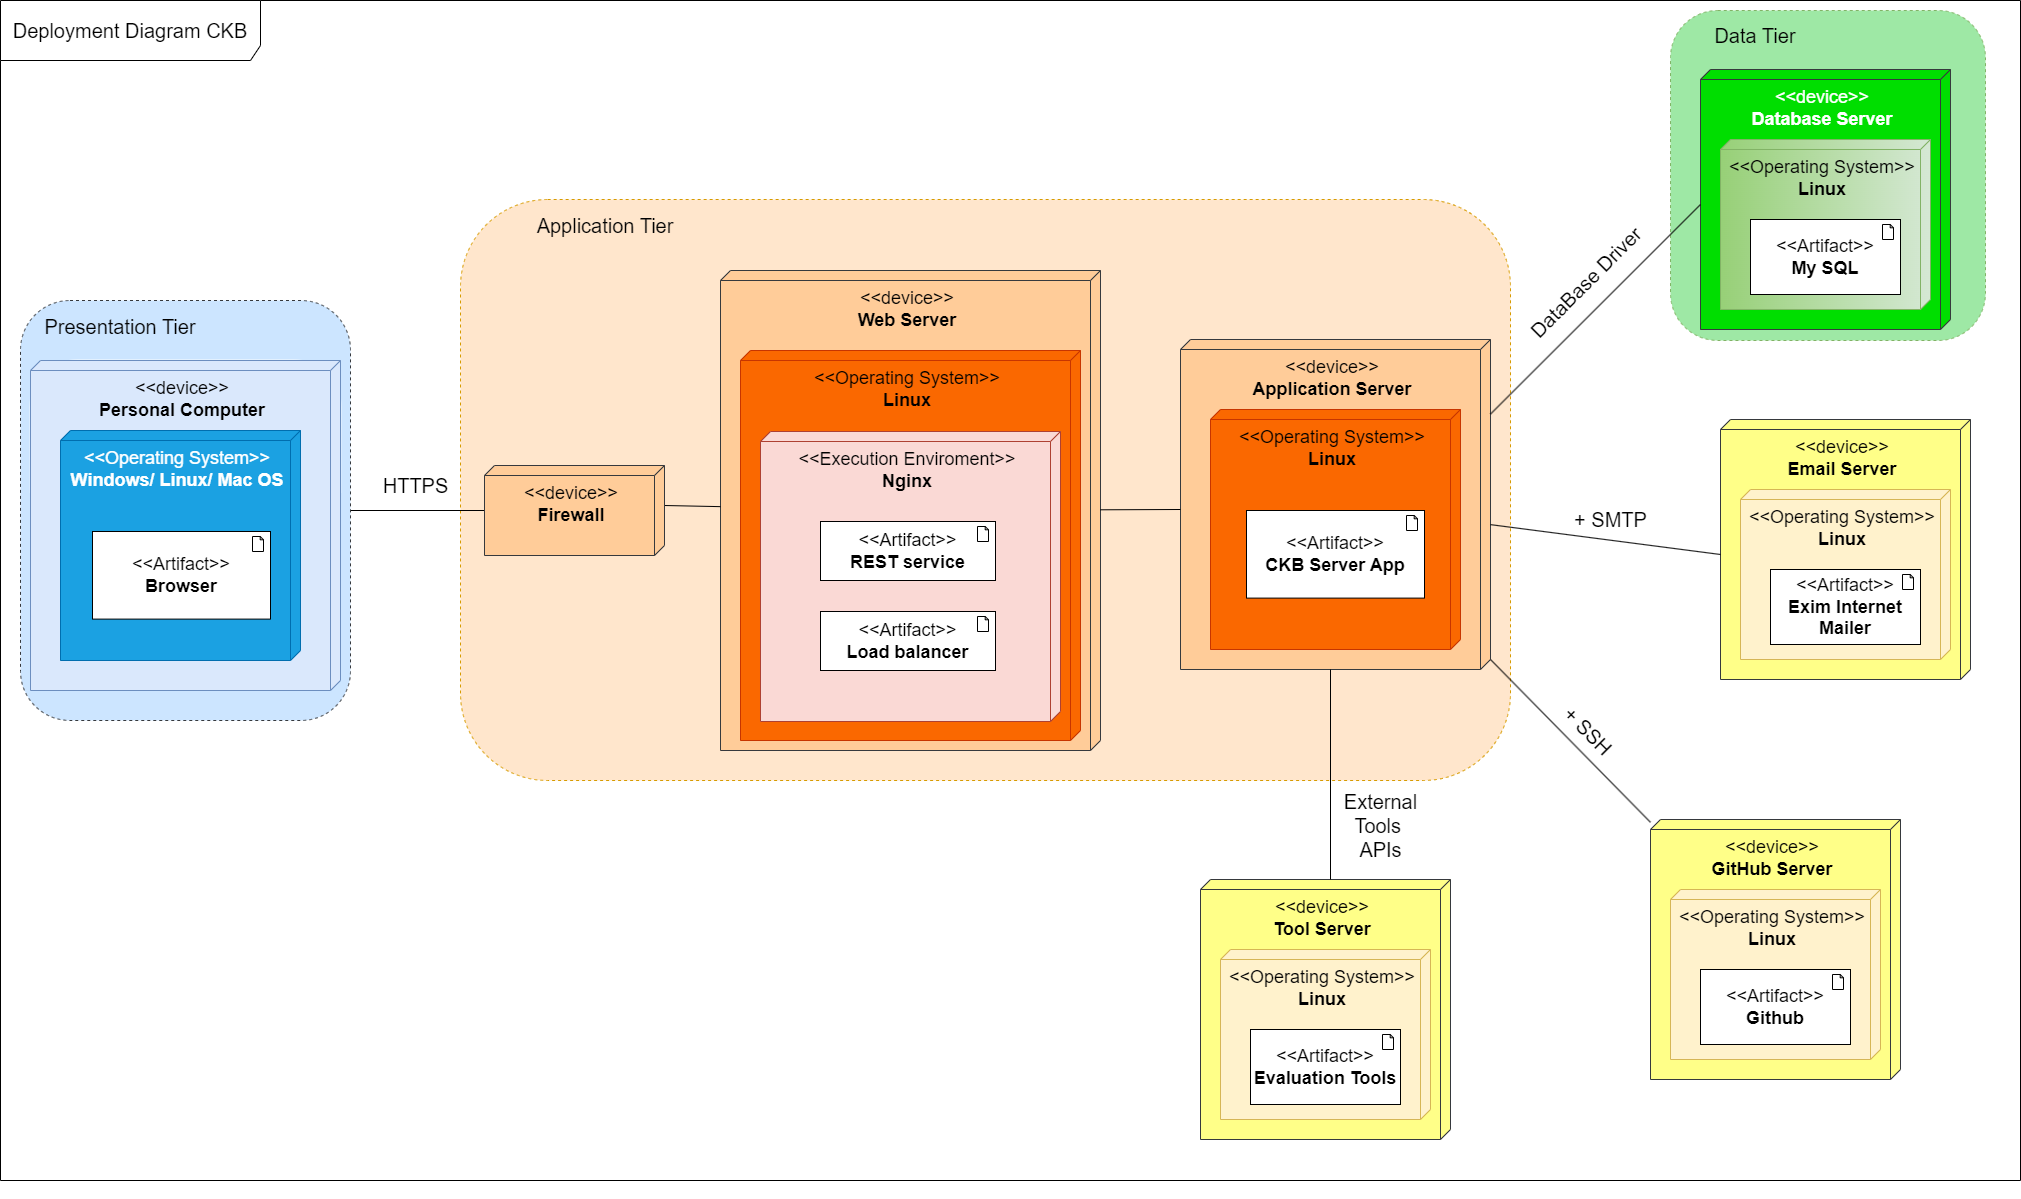
\includegraphics[width=1\linewidth]{CD_DD/DeploymentDiagram.png}
        \caption{Deployment Diagram.}
        \label{fig:Deployment_Diagram}%
    \end{center}
\end{figure}

\paragraph{Personal Computer:}
STs and EDs can access to the system by using any type of personal computer through their favorite web browser. The browser will communicate with the Web Server. Users can also use every device that allows them to search on a web browser, such as mobile phone, tablet, ecc.

\paragraph{Web Server:}
The Web Server provides access to the Application Server’s service to all the User that reaches the system through a web browser. In particular, the Web Server does not execute any business logic, but it simply does some load balancing on the receive requests from the client to the various Application Servers, in order to handle large User traffic.\\
It also provides to the client's browsers the HTML, JSON, Javascript and CSS files for making the rendering of the pages.

\paragraph{Firewall:}
It provides a way to limit the attack surface of any potential intruder by providing strict access rules.

\paragraph{Application Server:}
The application server contains the business logic of the entire system. Moreover, it communicates to the client through HTTPS protocol managed by the Web Server. The various requests coming from the Web Server are routed to the corresponding module thanks to the Dashboard Manager.\\
Furthermore, it communicates to the Database Server through the model gateway. This node is replicated in order to handle large user traffic.

\paragraph{Database Server:}
All the Data about Tournaments, Battles, Users, Groups and Badges are stored into the Database Server and managed by MySQL.\\
The various Application Servers can retrieve information on this node through the model module and the database driver.

\paragraph{Email Server:}
After the registration, Users have to click on the link sent by eMail to confirm their profile. The Application Server, immediately after the registration, contacts the Email Server through SMTP protocol to send the confirmation eMail to the User.

\paragraph{Github Server:}
The dialogs with the Application Server node occur during the different Battle phases: when the ED creates a new Battle also a GitHub repository is created containing the code kata of the Battle and it is subsequently forked from the various STG.\\
The GitHub Server is also periodically contacted for retrieving newly committed code on the main branch of the different STGs' repositories.
For those scopes, the Application Server shall communicate with the Github Server through the SSH protocol.


\paragraph{Tool Server:}
With the External Tool APIs the Application Server can contact the Tool Server and pass to it the code retrieved from the Github Server to be tested and evaluated.

\newpage
\section{Runtime View}
\label{sec:runtime_view}%

\subsection{SignUp as ED}
\begin{figure}[H]
    \begin{center}
        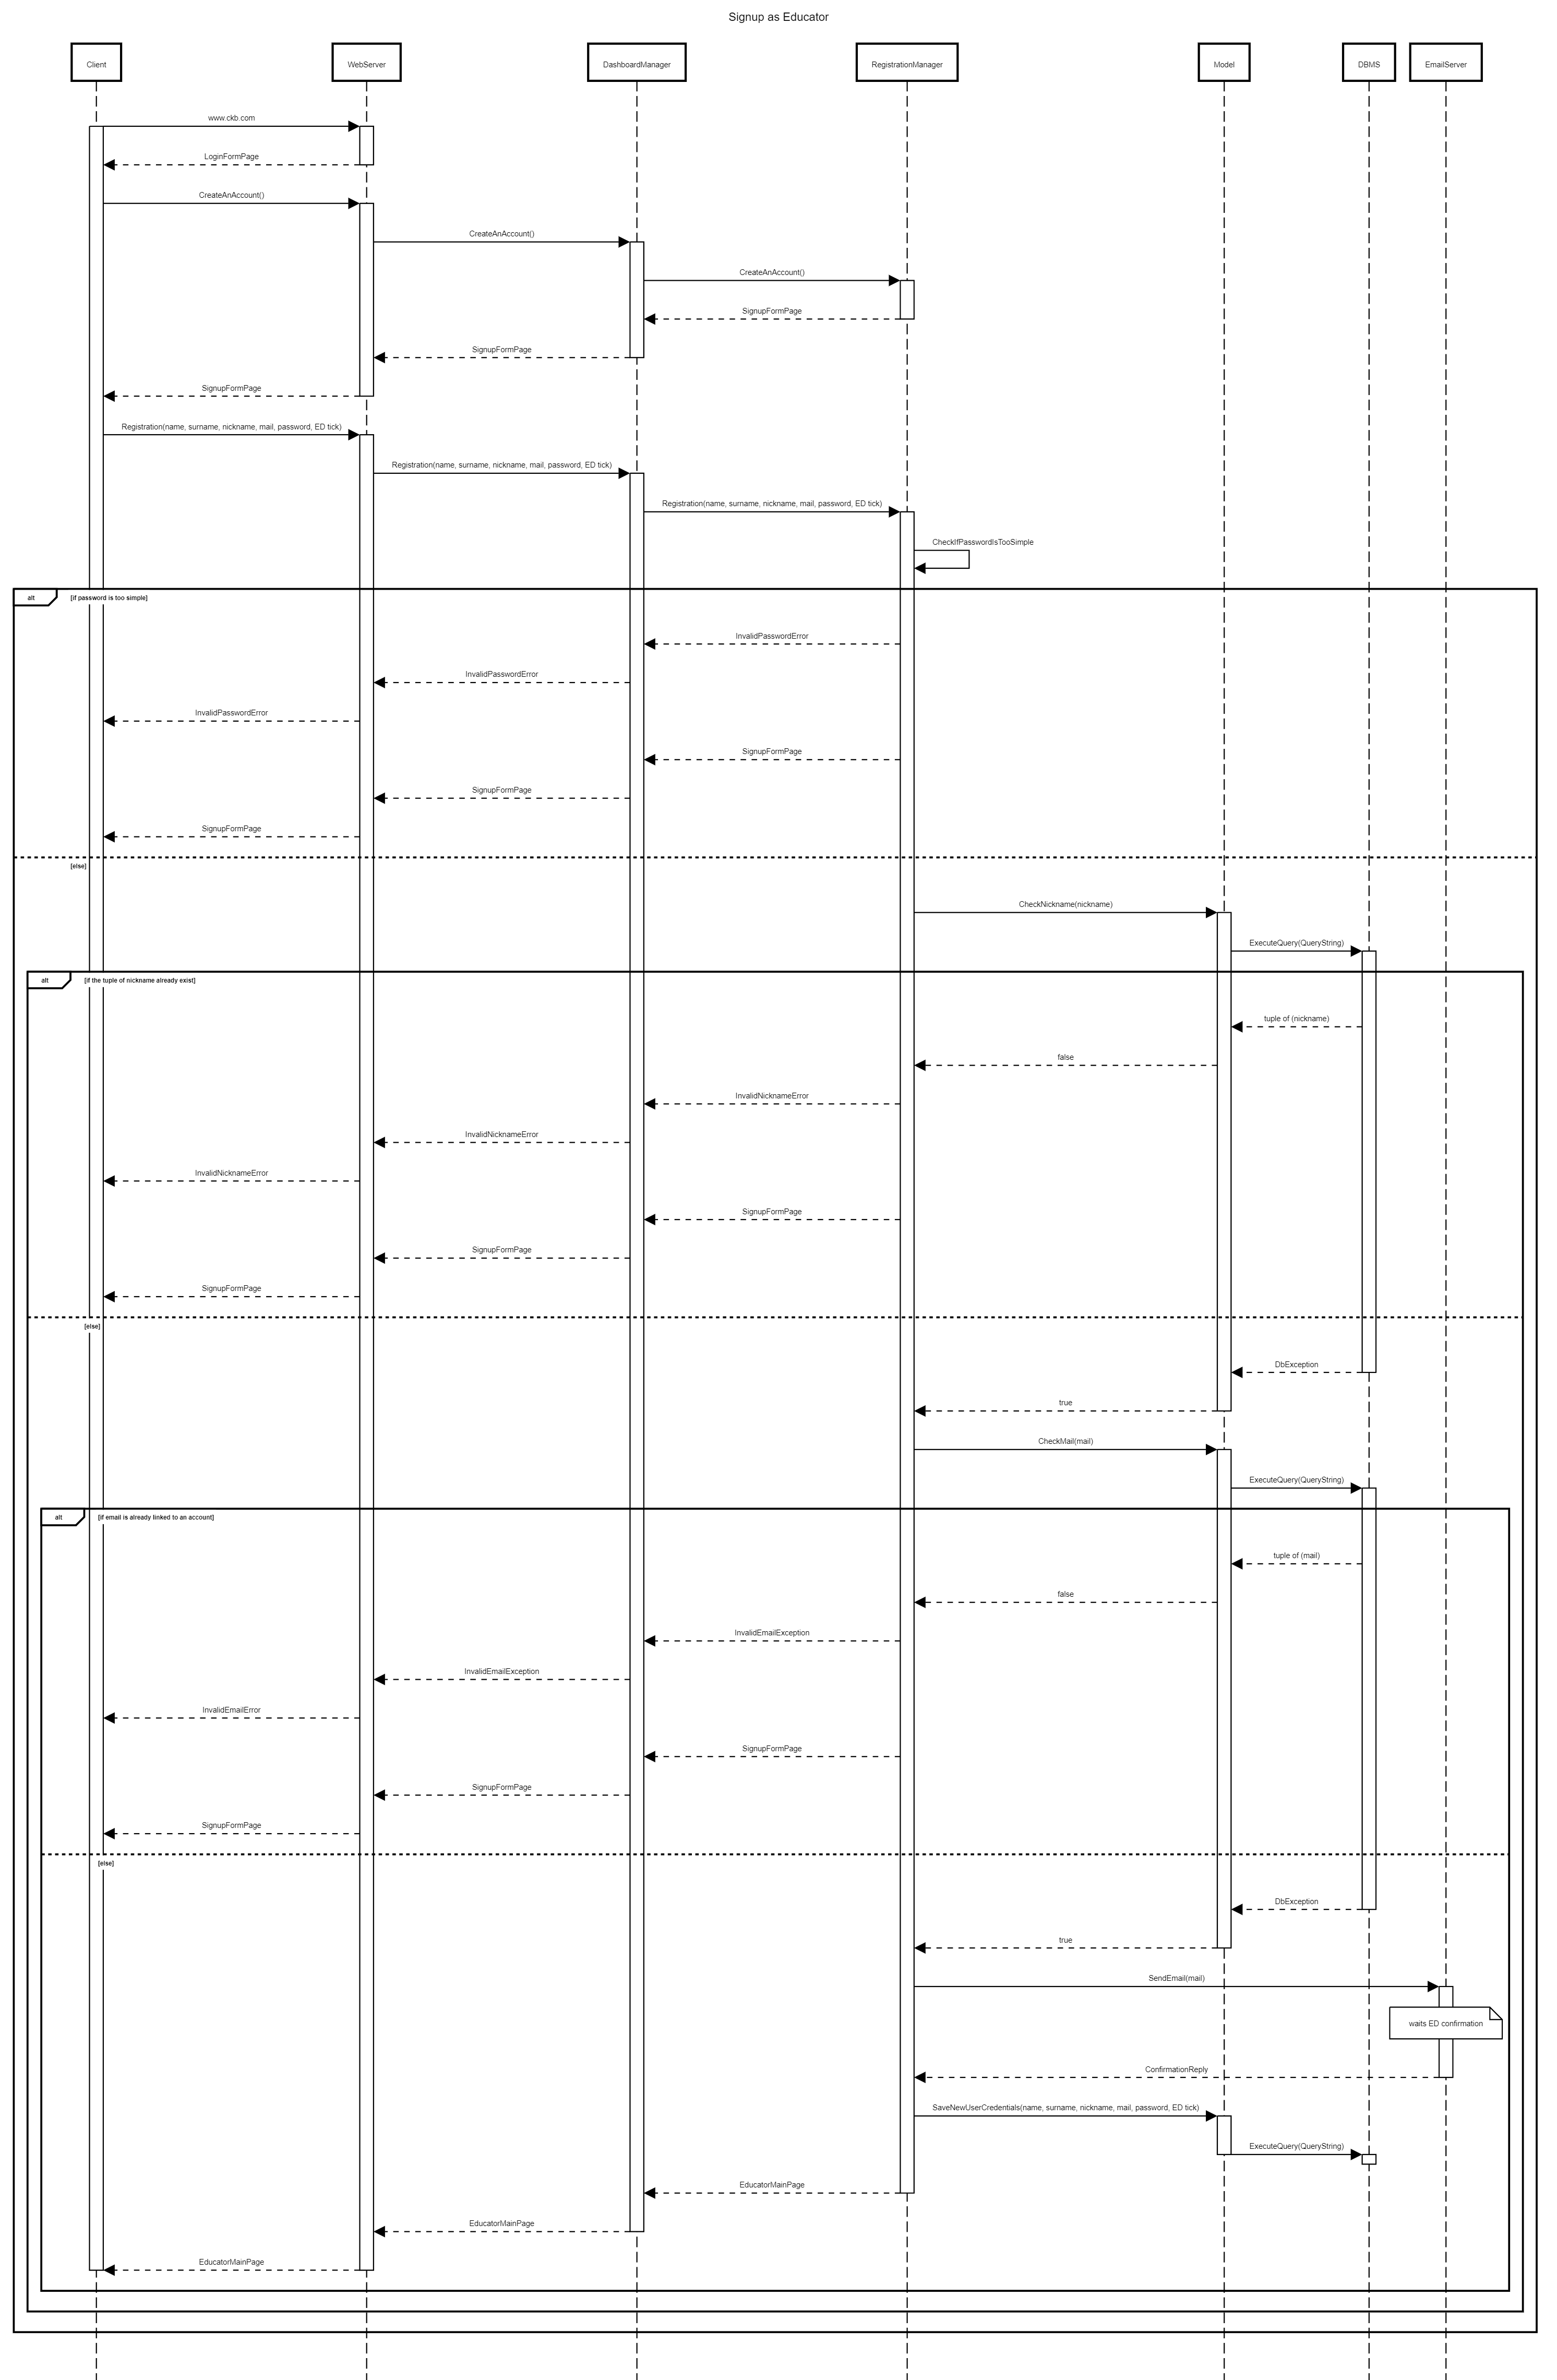
\includegraphics[width=0.8\linewidth]{RuntimeView/SignupED.png}
        \caption{Runtime view for 'SignUp as ED'.}
        \label{fig:runtime_signupasED}%
    \end{center}
\end{figure}

This sequence diagram represents the ED registration process.
The ED searches into the browser for the CKB Landing page and gets redirected to the “Login” page. After clicking on the "Create Account" button is redirected to the signup form. The ED fills out the form with his data, such as name, surname, nickname, mail and password and he ticks on the “Register as an Educator” option.
This form is forwarded to the DashboardManager that redirects the request to the RegistrationManager component. It does various checks on the sended parameters and, if everything is correct, sends an eMail to confirm  the registration. If the link in the mail is clicked the RegistrationManager saves the new profile into the Database (passing through the Model component that connects the Application Server with the DBMS) and shows to the ED the ED Homepage.


\subsection{SignUp as ST}
\begin{figure}[H]
    \begin{center}
        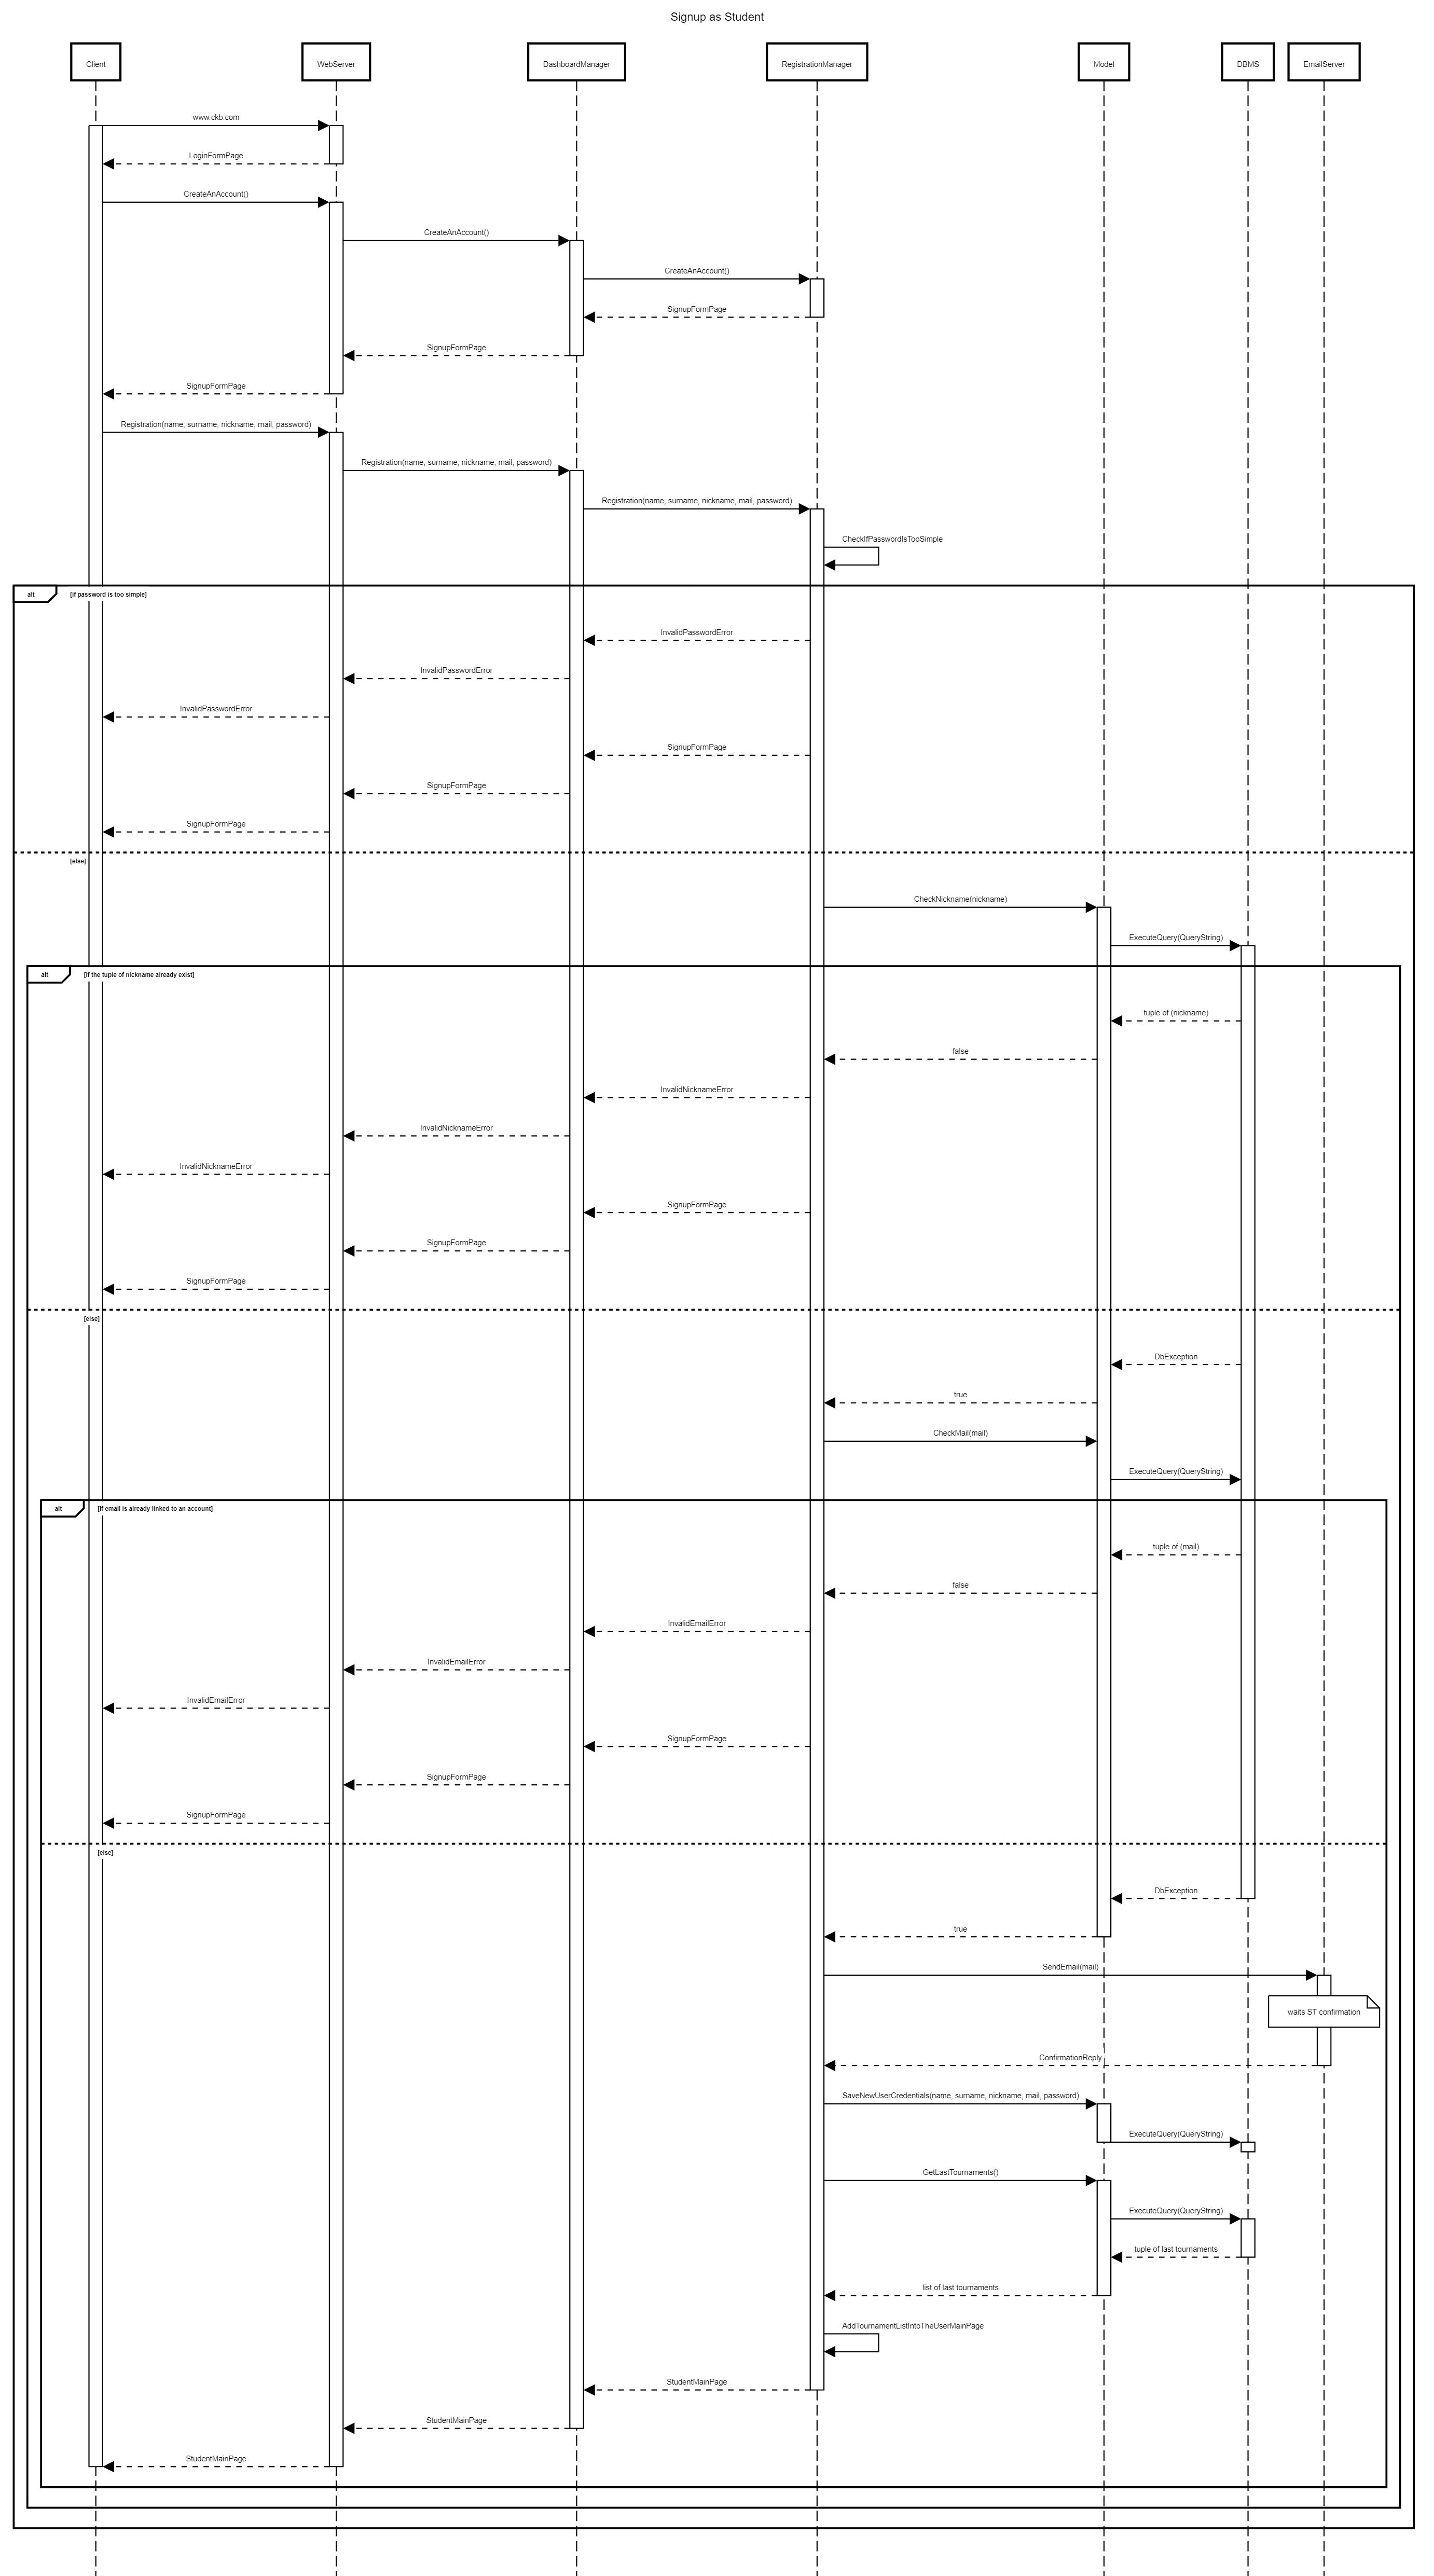
\includegraphics[width=0.8\linewidth]{RuntimeView/SignupAsST.png}
        \caption{Runtime view for 'SignUp as ST'.}
        \label{fig:runtime_signupasST}%
    \end{center}
\end{figure}

This sequence diagram represents the ST registration flow.
The ST searches into the browser for the CKB Landing page and gets the “Login” page.
After clicking on the "Create Account" button is redirected to the signup form.
The ST fills out the form with its data, such as name, surname, nickname, mail and password. 
This form is forwarded to the DashboardManager that redirects the request to the RegistrationManager component. It does various checks on the sended parameters and, if everything is correct, sends an eMail to confirm the registration.
If the link in the mail is clicked the RegistrationManager saves the new profile into the Database (passing through the Model component that connects the Application Server with the DBMS) and shows to the ST the ST Homepage.

\subsection{Login}
\begin{figure}[H]
    \begin{center}
        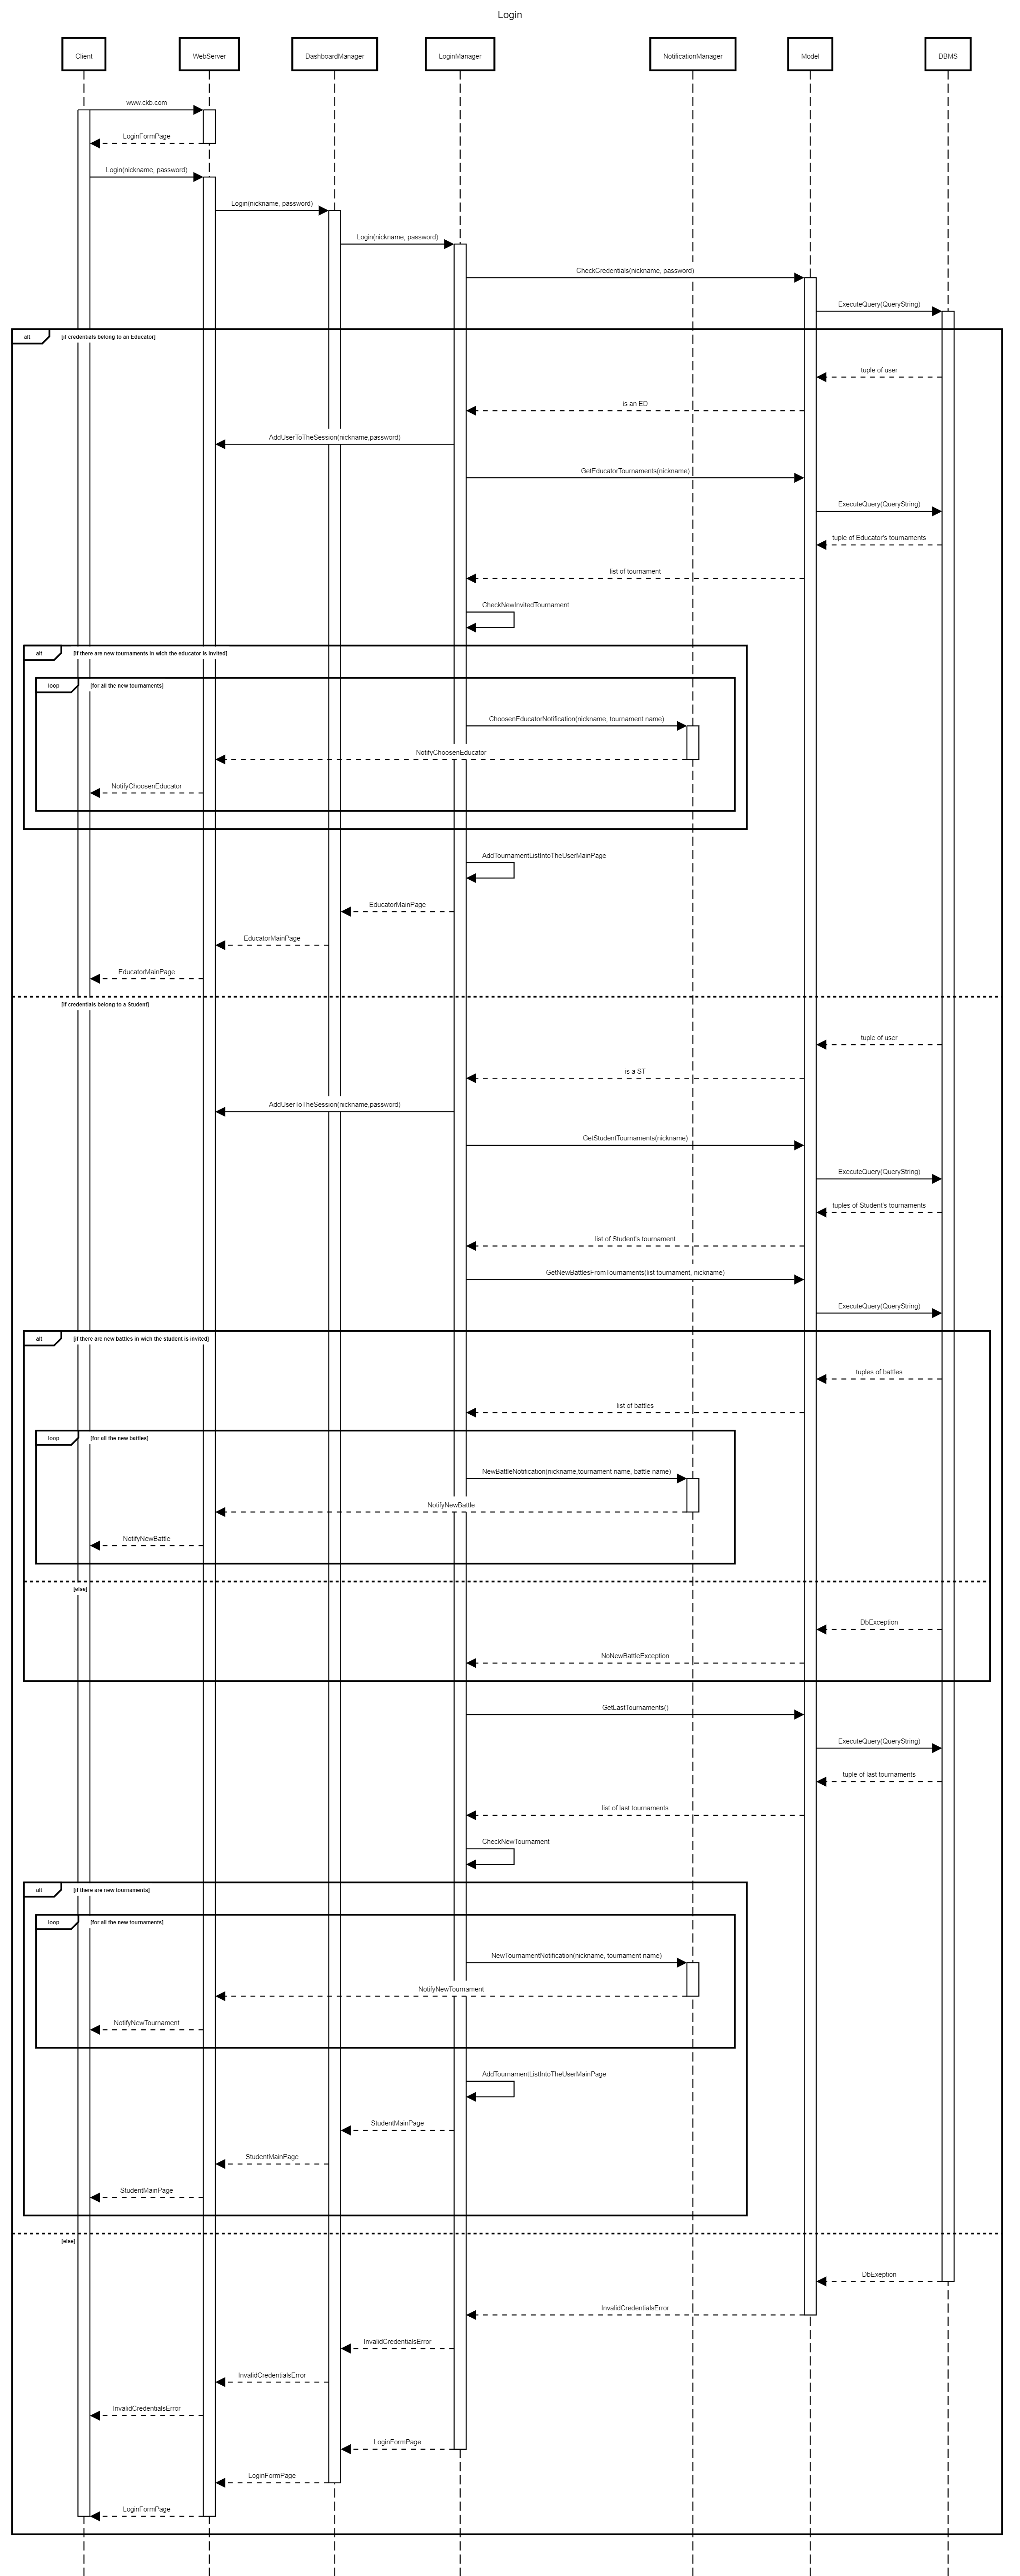
\includegraphics[height=0.8\pdfpageheight, width=0.8\linewidth]{RuntimeView/Login.png}
        \caption{Runtime view for 'Login'.}
        \label{fig:runtime_login}%
    \end{center}
\end{figure}
In this sequence diagram is explained how the login operation works.
The User searches into the browser for the CKB Landing page and gets the login page.
The User fills out the form with his credentials (nickname and password) and he sends it to the DashboardManager that redirects the request to the LoginManager that checks the credentials through the Model component.
The Model retrieves the User information from the DBMS and indicates to the LoginManager if the user is an ED or a ST.
The LoginManager adds the User credentials into the User session and retrieves the notifications that the User has missed and shows them to him.
After that the LoginManager gets from DBMS the information for creating the two types of User main page and sends them to the User.


\subsection{Create a Tournament}
\begin{figure}[H]
    \begin{center}
        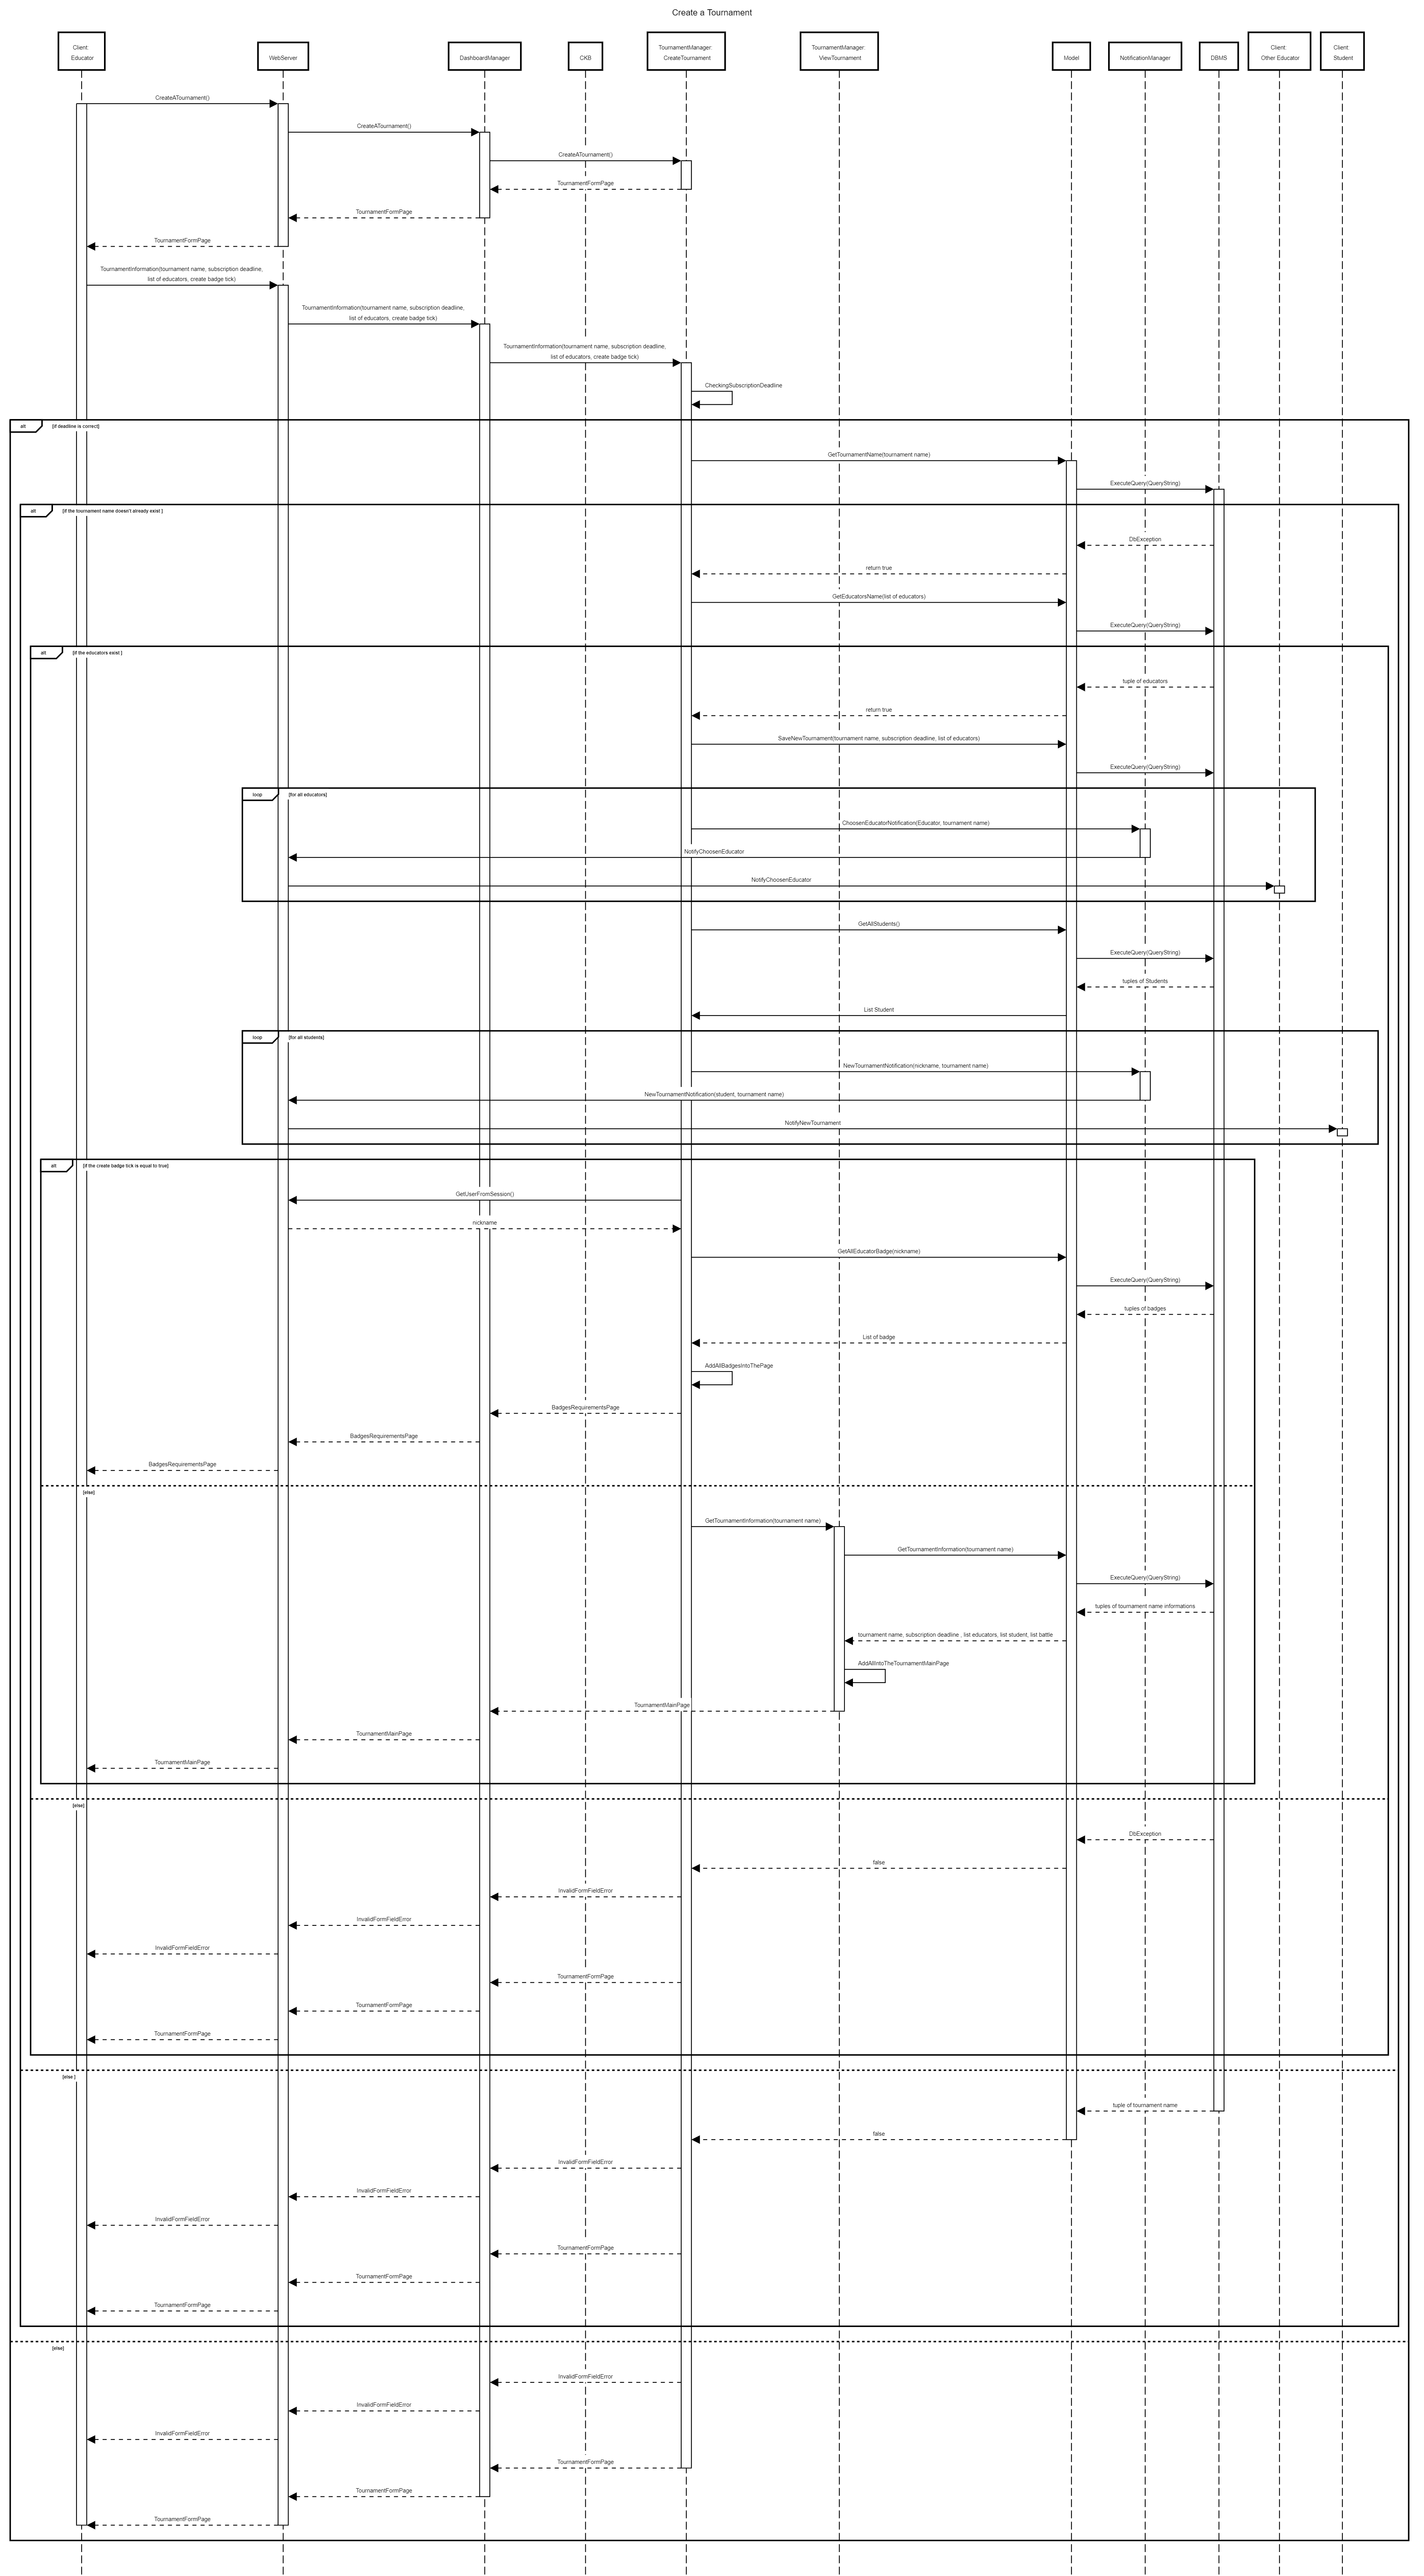
\includegraphics[width=0.8\linewidth]{RuntimeView/CreateTournament.png}
        \caption{Runtime view for 'Create a Tournament'.}
        \label{fig:runtime_createtournament}%
    \end{center}
\end{figure}
This sequence diagram represents the flow behind the create Tournament process.
The ED clicks on the “Create a new Tournament” button into the “ED Homepage” for retrieving the create Tournament form from the CreateTournament module. The ED fills out the form with the new Tournament information (Tournament name, subscription deadline, list of EDs) and if he wants to create or modify some Badges he ticks the “Create Badges for this Tournament” option. The form is sent to the DashboardManager that redirects the request to the CreateTournament module that, if the all parameters are corrects, saves the new Tournament into the DBMS and sends a notifications through the NotificationManager to all the invited EDs and to all the STs.
If the “Create Badges for this Tournament” option is ticked, the  CreateTournament module retrieves the ED’s Badges and redirects the ED to the “Create Badge” Page, if not the CreateTournament module calls the ViewTournament module in order to show the “ED Tournament” Page.


\subsection{Join a Tournament}
\begin{figure}[H]
    \begin{center}
        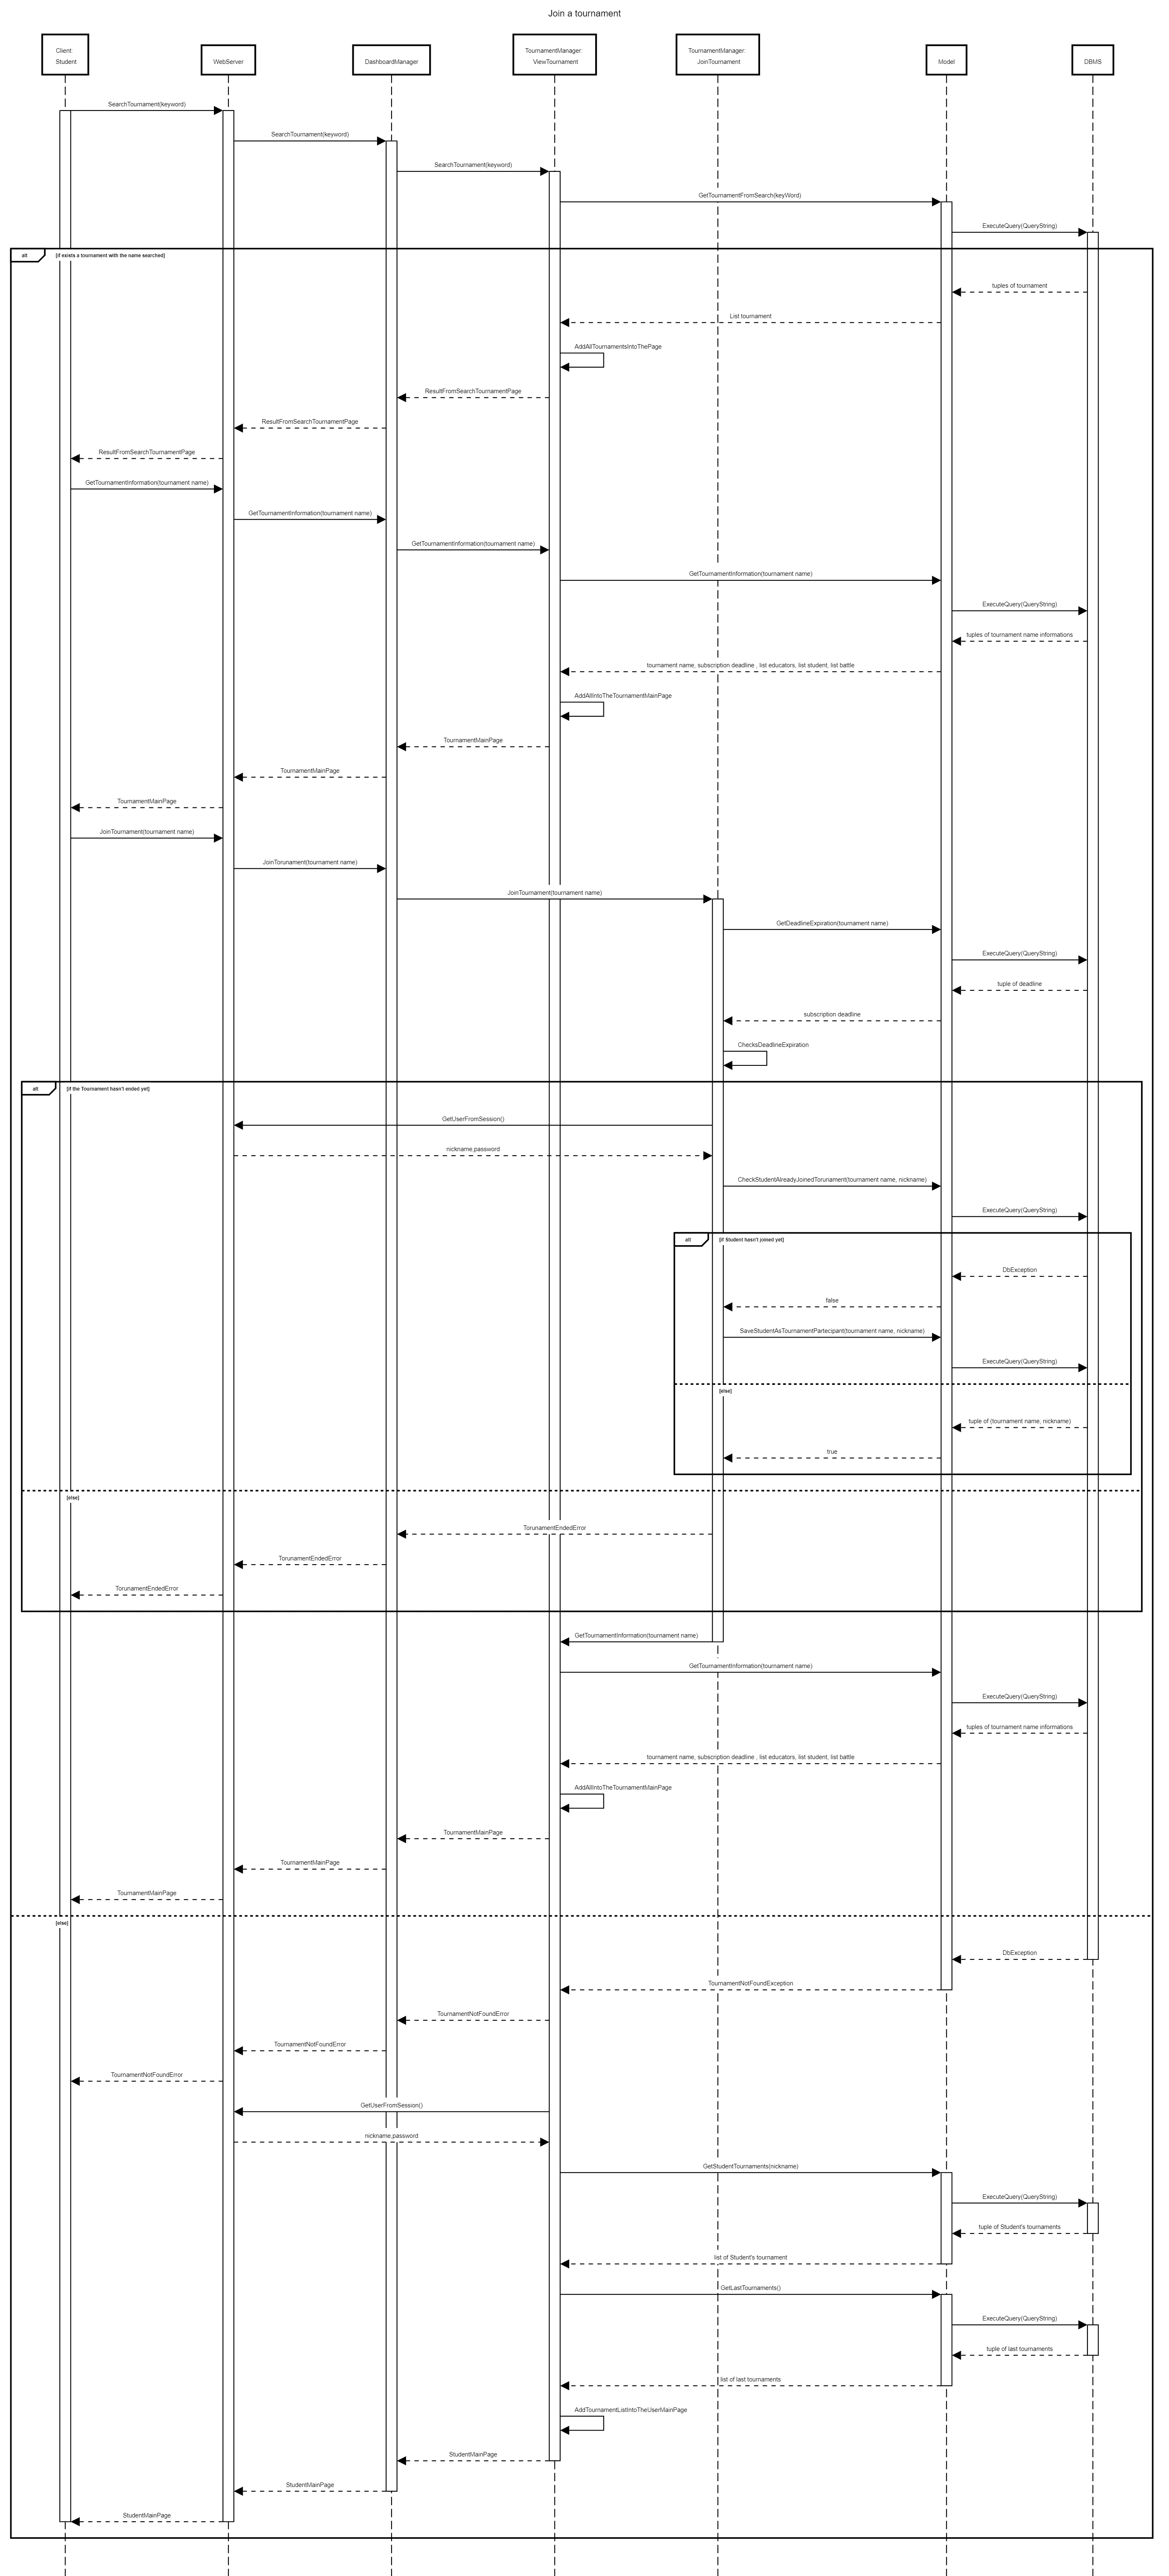
\includegraphics[height=0.8\pdfpageheight]{RuntimeView/JoinTournament.png}
        \caption{Runtime view for 'Join a Tournament'.}
        \label{fig:runtime_jointournament}%
    \end{center}
\end{figure}
This sequence diagram represents the flow behind the ‘Join Tournament’ operation for a ST.
The ST types a keyword into the search bar and sends it to the DashBoardManager that redirects the request to the ViewTournament module.
The ViewTournament module retrieves from the DBMS the list of Tournaments that corresponds to the searched keyword and, if it is not empty, shows it to the ST. The ST clicks on a Tournament and the ViewTournament module retrieves the information of that tournament from DBMS and shows them to the ST. The ST clicks on the “Join Tournament” button and his request is sent to the JoinTournament module that does some checks on the ST and in the Tournament. If all checks are passed the ST is saved into the DBMS as a Tournament participant and the “ST Tournament” page is shown to him through the ViewTournament module.


\subsection{Create a Battle}
\begin{figure}[H]
    \begin{center}
        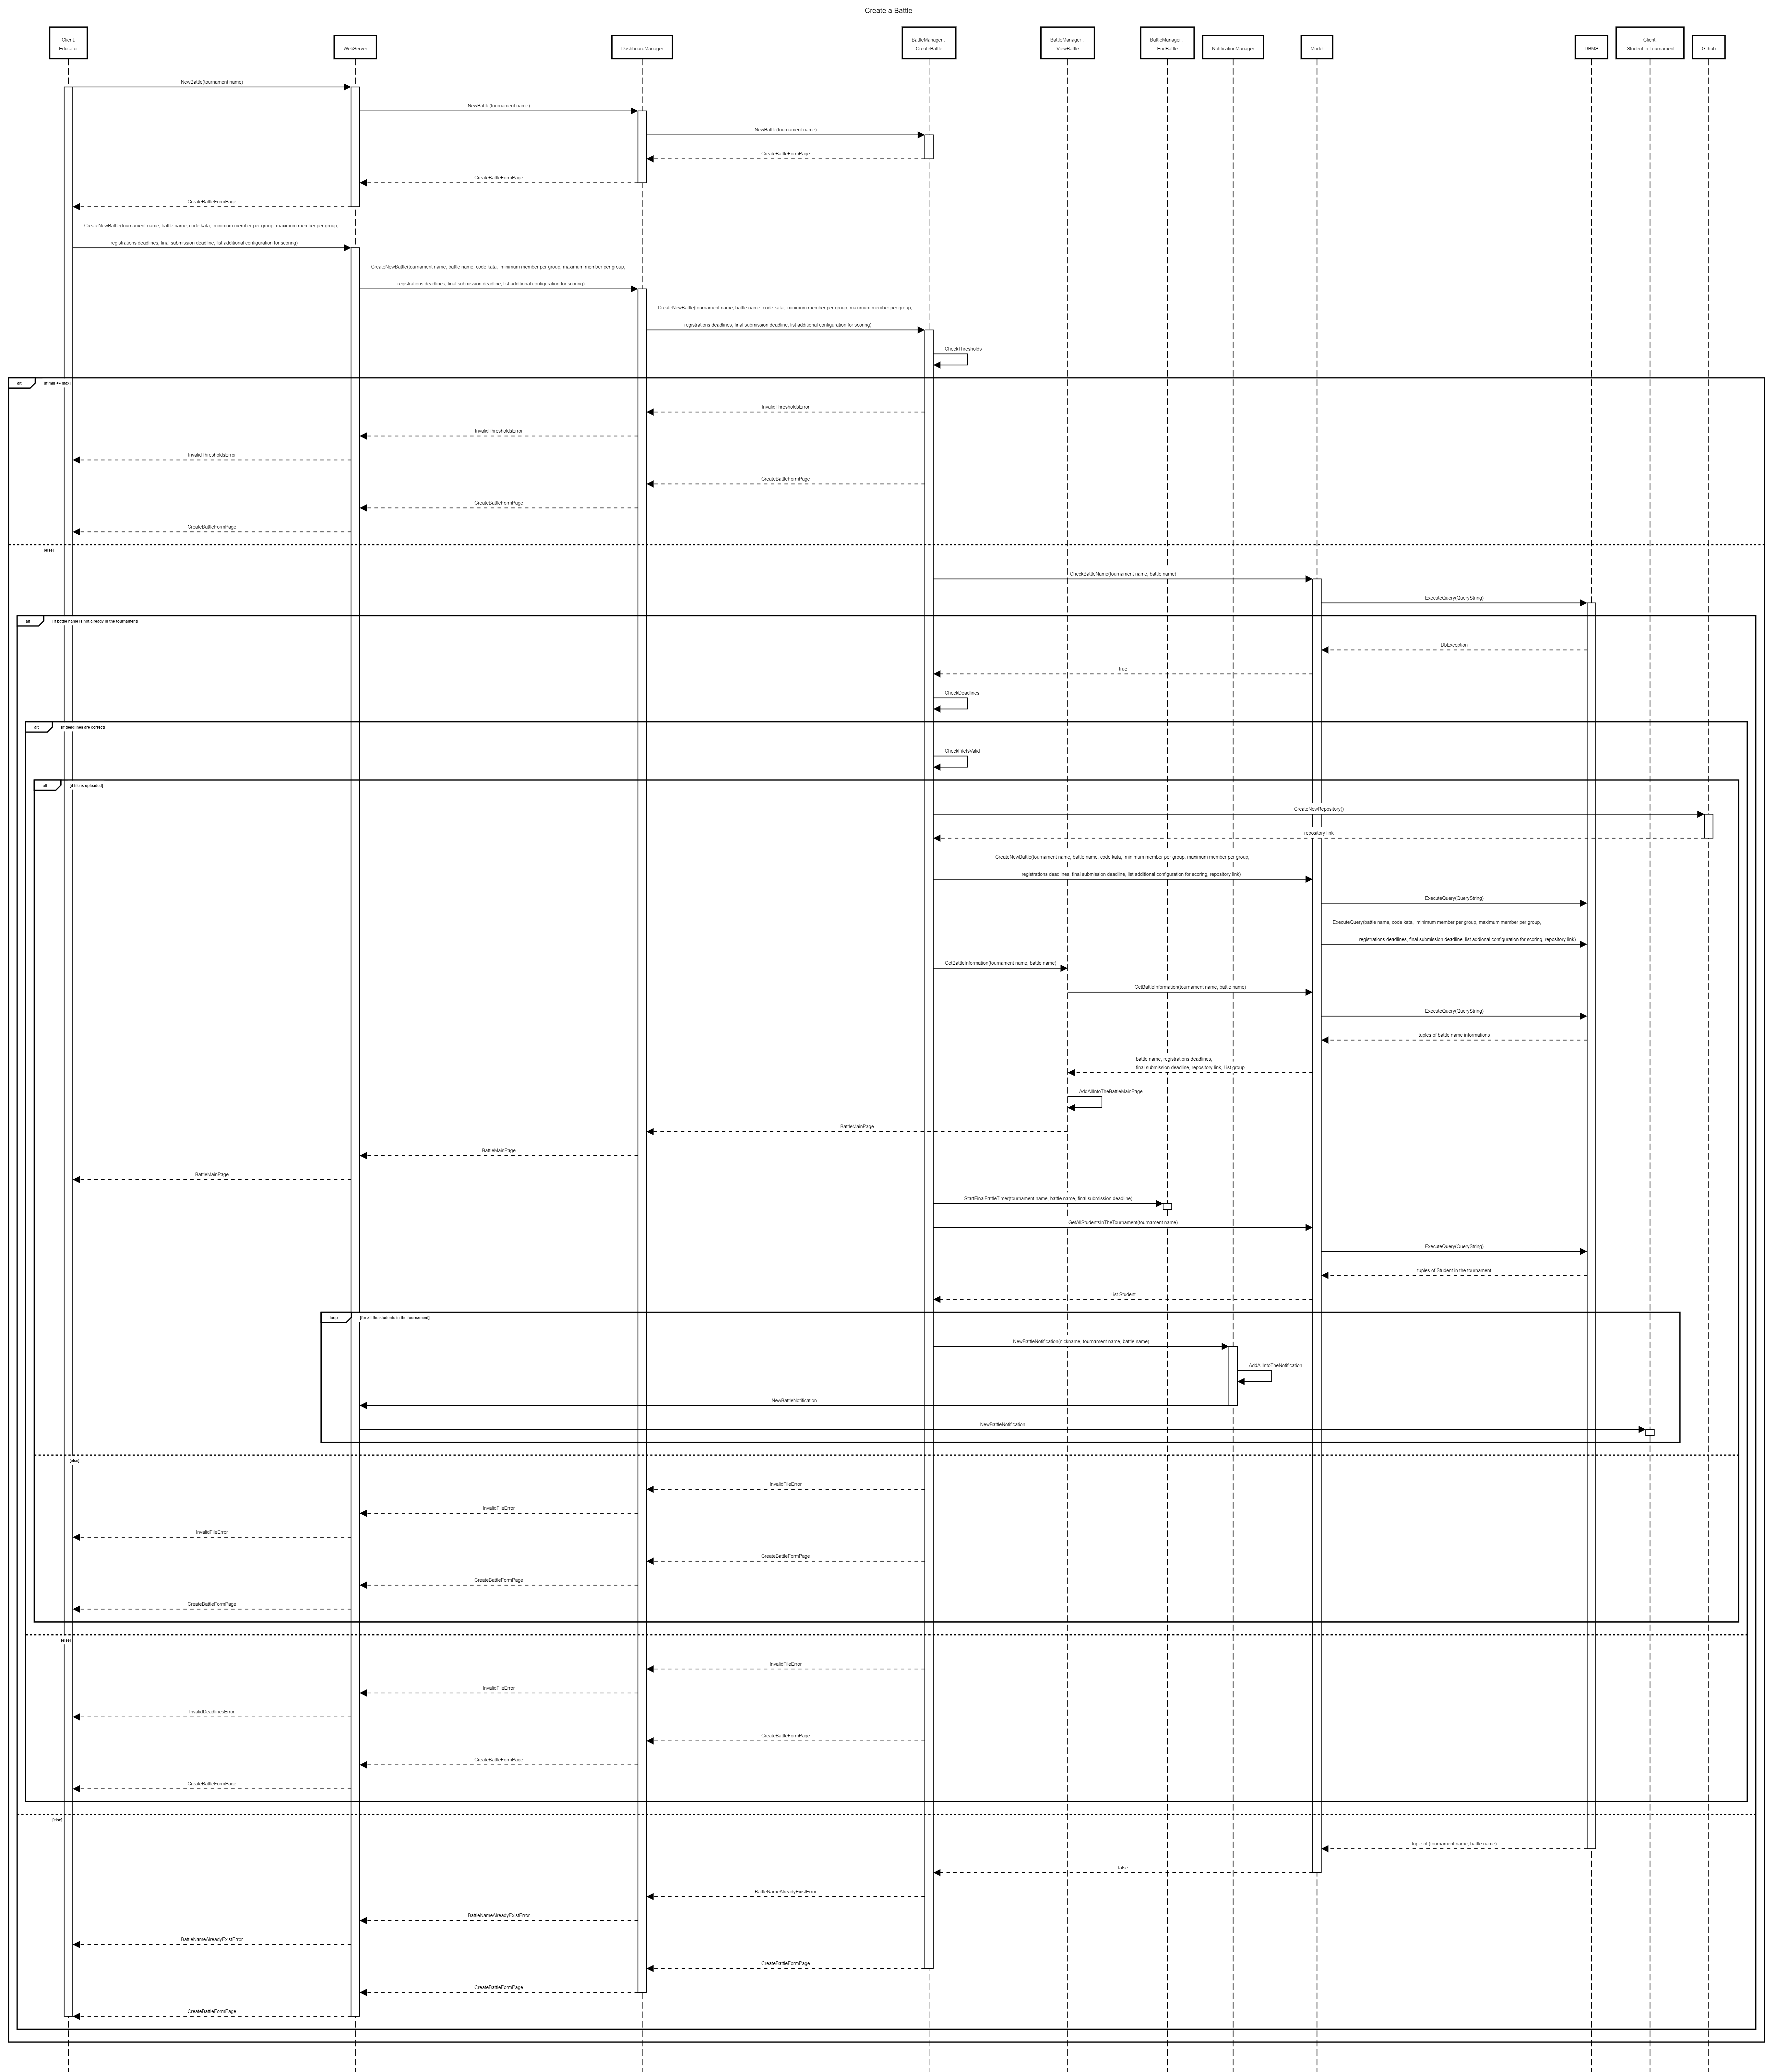
\includegraphics[width=0.8\linewidth]{RuntimeView/CreateBattle.png}
        \caption{Runtime view for 'Create a Battle'.}
        \label{fig:runtime_createbattle}%
    \end{center}
\end{figure}
This sequence diagram represents the flow behind the ‘Battle creation’ 
process. The ED clicks on the “Create a new Battle” button into the “ED Tournament” page. His request is processed by the CreateBattle module that redirects the ED to the Create Battle Form. The ED inserts the new Battle information (Battle name, code kata,  minimum member per group, maximum member per group, registrations deadlines, final submission deadline, list additional configuration for scoring) into the form and sends it to the CreateBattle module. The CreateBattle module does some checks on these informations and if they are all correct he creates a new GH repository and it retrieves the repository link. After this, The CreateBattle module saves the new Battle into the Database (passing through the Model and then the DBMS) and it shows the “ED Battle” page. The CreateBattle module also starts the timer on the EndBattle module and finally it contacts, through the Notification Manager, all the STs in the Tournament to notify them about the start of a new Battle.



\subsection{Join a Battle}
\begin{figure}[H]
    \begin{center}
        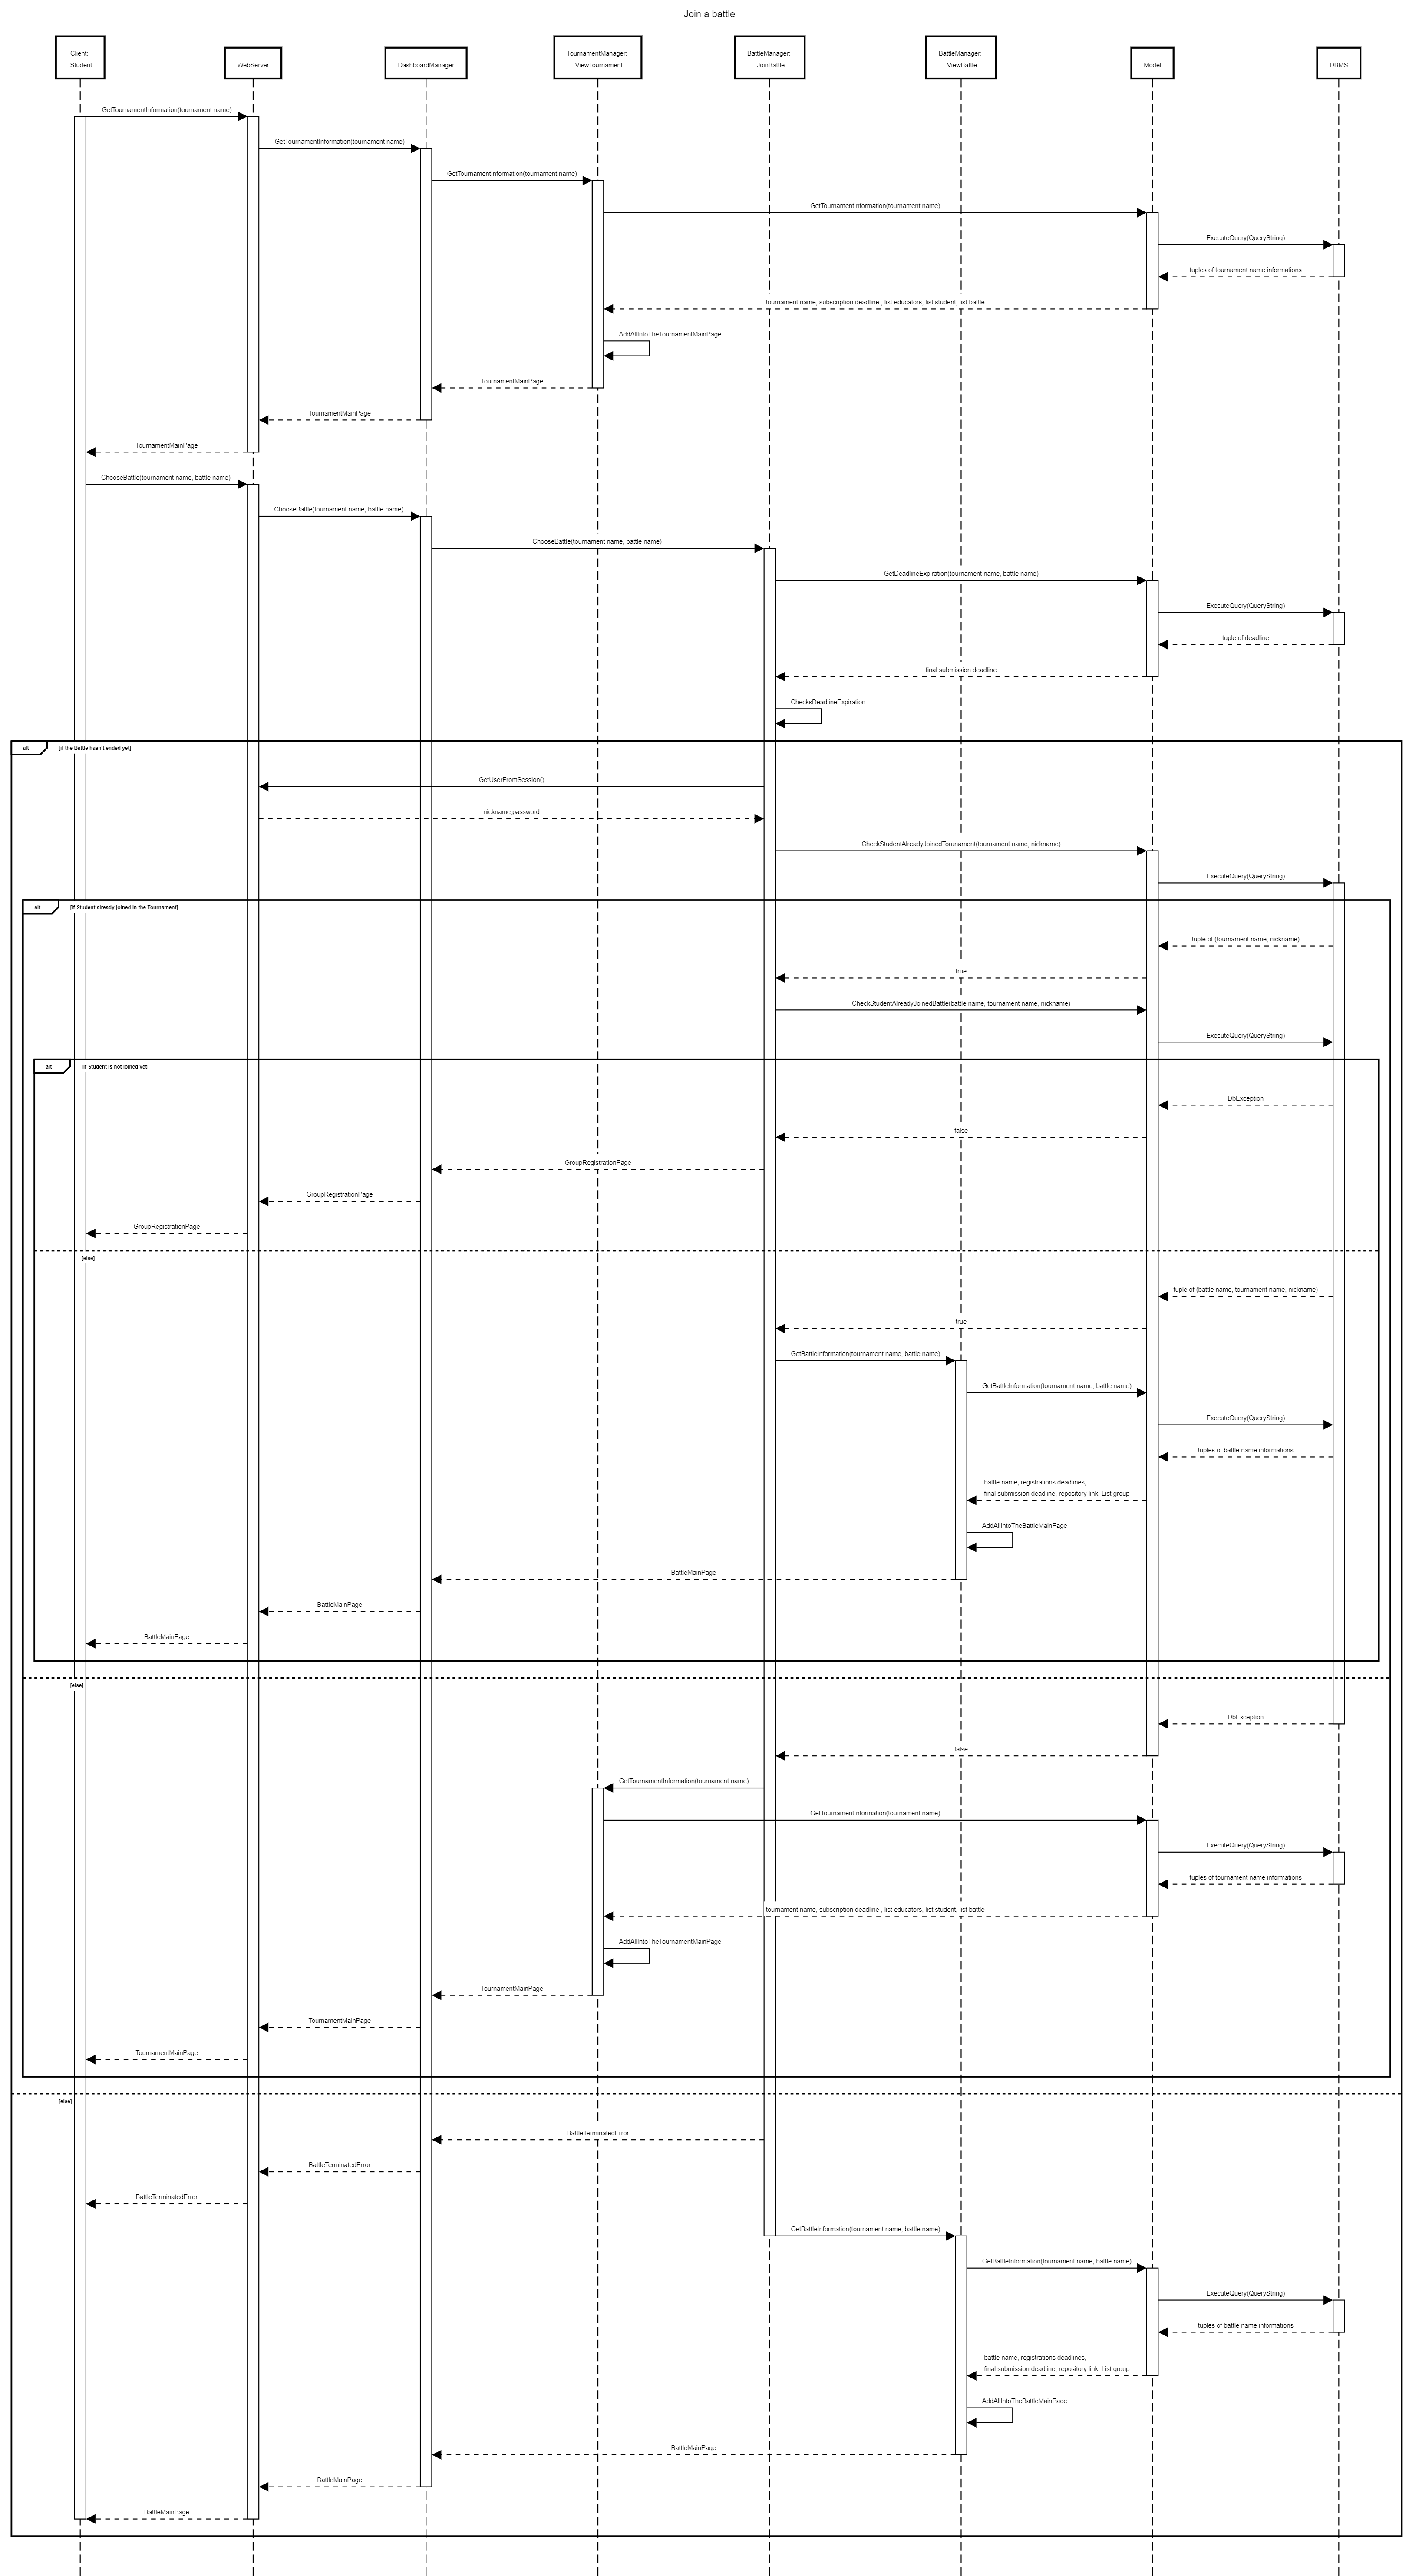
\includegraphics[width=0.8\linewidth]{RuntimeView/JoinBattle.png}
        \caption{Runtime view for 'Join a Battle'.}
        \label{fig:runtime_joinbattle}%
    \end{center}
\end{figure}
This sequence diagram represents the flow behind the ‘Join Battle’ operation for a ST. The ST clicks on a Tournament and the ViewTournament module shows him the “ST Tournament” page. Then the ST clicks on the “Join Battle” button next to the Battle’s name and then the JoinBattle module does the proper checks on the Battle and ST data. If all checks are correct, then the JoinBattle module redirects the ST to the “Create Group” page.


\subsection{Create a group and Battle confirmation}
\begin{figure}[H]
    \begin{center}
        \includegraphics[height=0.8\pdfpageheight]{RuntimeView/CreateGroup.png}
        \caption{Runtime view for 'Create a group and Battle confirmation'.}
        \label{fig:runtime_creategroup}%
    \end{center}
\end{figure}
This sequence diagram represents the flow behind the phase in which, after the fulfillment of the ‘Join Battle’ operations, the ST creates a STG and confirms his participation in the battle.
The ST fills out the Create Group form with some group information (such as group name, list of invited STs nicknames) and then sends it to the CreateGroup module.
The CreateGroup module does some checks on the information coming from the form and then it sends invitations through the Notification Manger to the other STs. If a ST accepts the invitation the CreateGroup module adds the ST to the group and shows to the group creator that the ST has accepted the invitation. If a ST rejects the invitation or if the STG is already full the CreateGroup module shows to the group creator that the ST has rejected the invitation. When the group is formed the ST can click on the “Confirm Group” button and the CreateGroup module adds the group into the Battle and calls the ViewBattle module for showing the Battle main page to the ST.


\subsection{Open a profile}
\begin{figure}[H]
    \begin{center}
        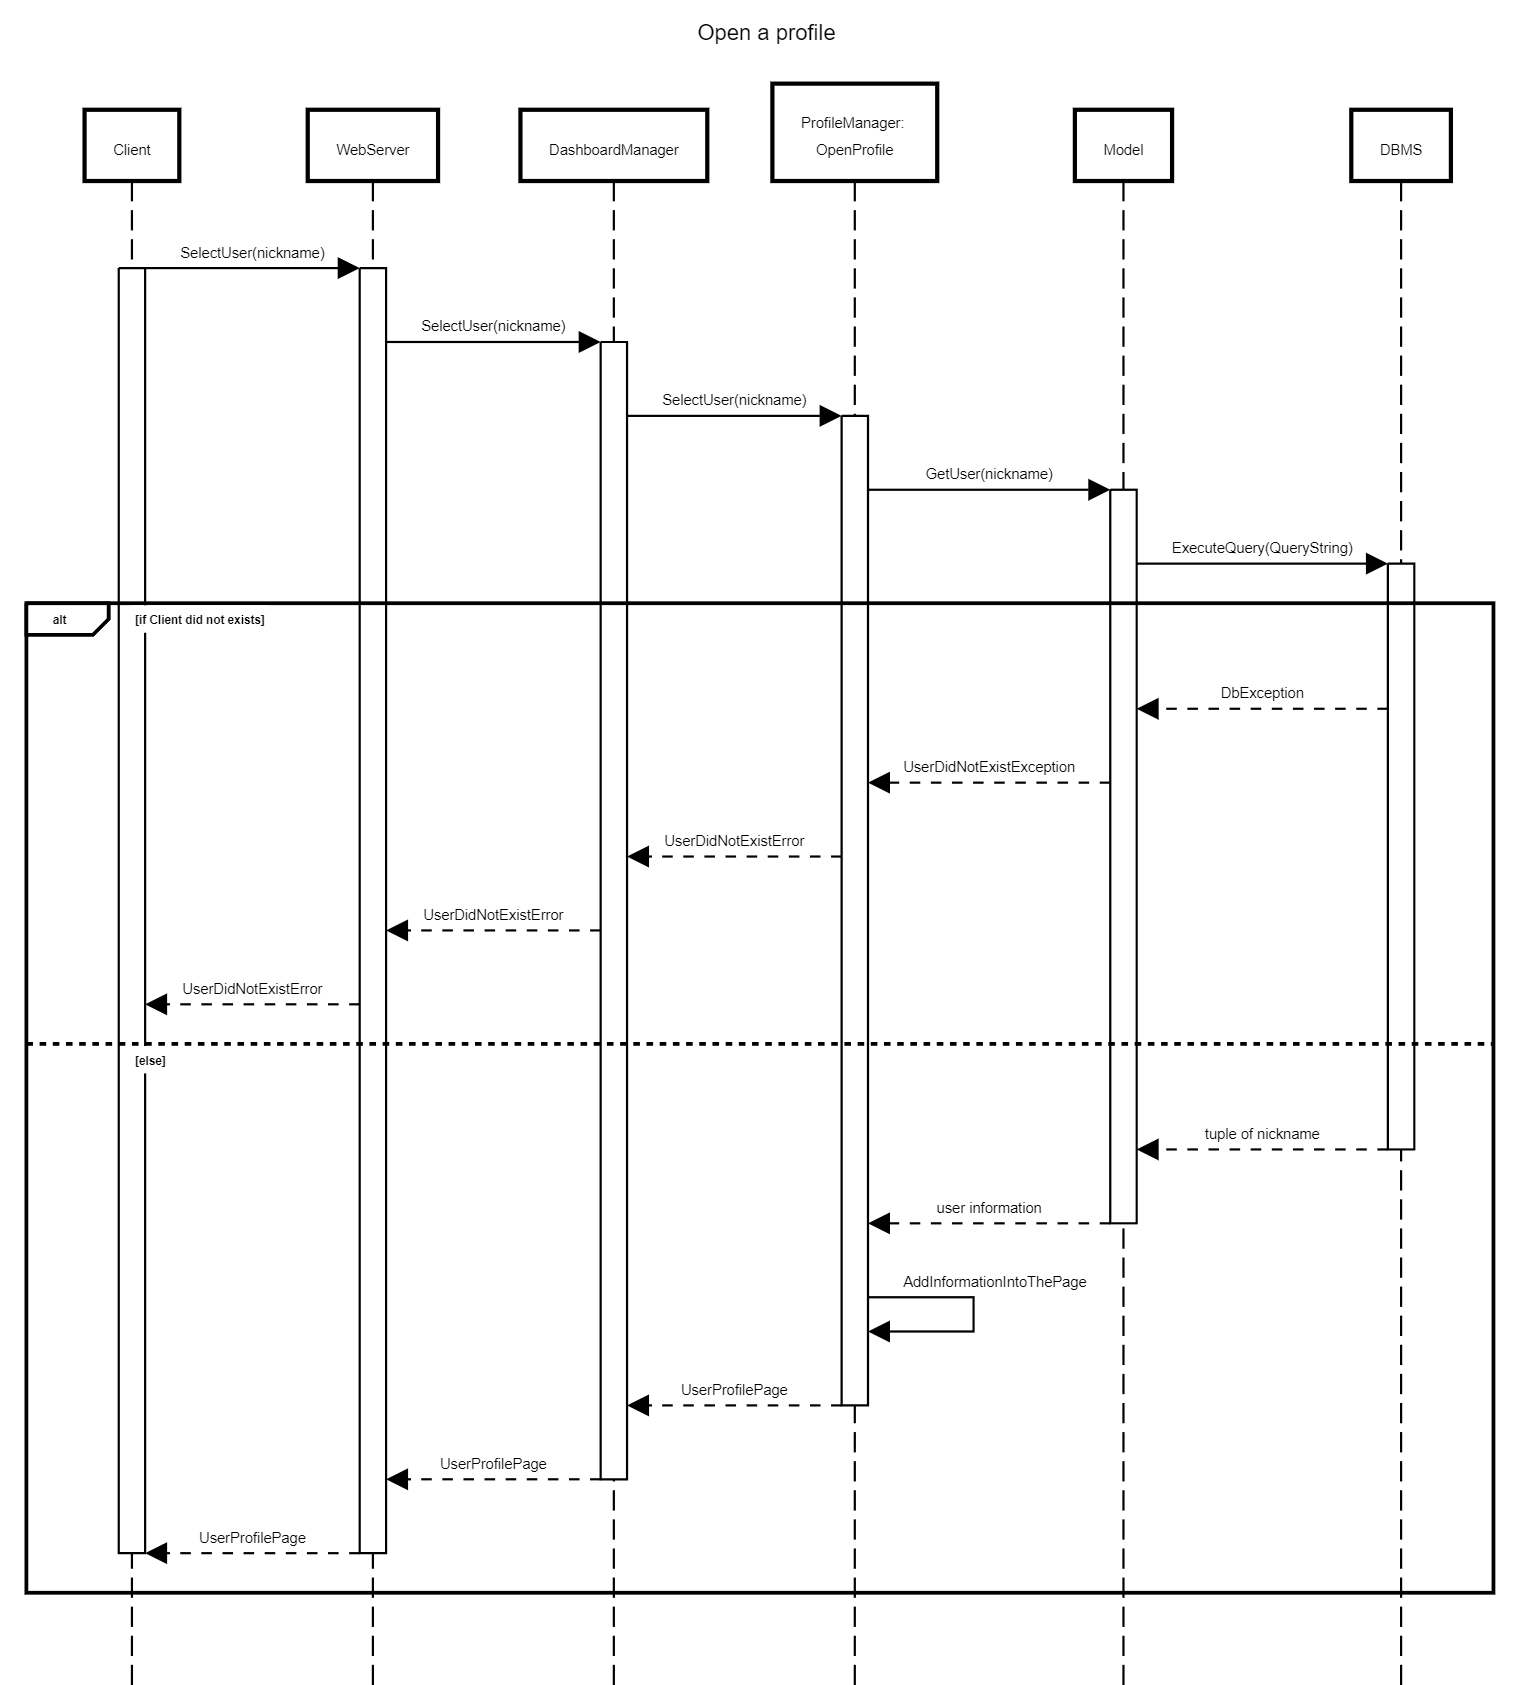
\includegraphics[width=0.8\linewidth]{RuntimeView/OpenProfile.png}
        \caption{Runtime view for 'Open a profile'.}
        \label{fig:runtime_openprofile}%
    \end{center}
\end{figure}
This sequence diagram represents the User open profile process.
The User selects a nickname from the User list and sends it to the DashBoardManager that redirects the request to the OpenProfile module.
The OpenProfile module retrieves from the DBMS the information of the selected User and shows it to the User.


\subsection{Search for a profile}
\begin{figure}[H]
    \begin{center}
        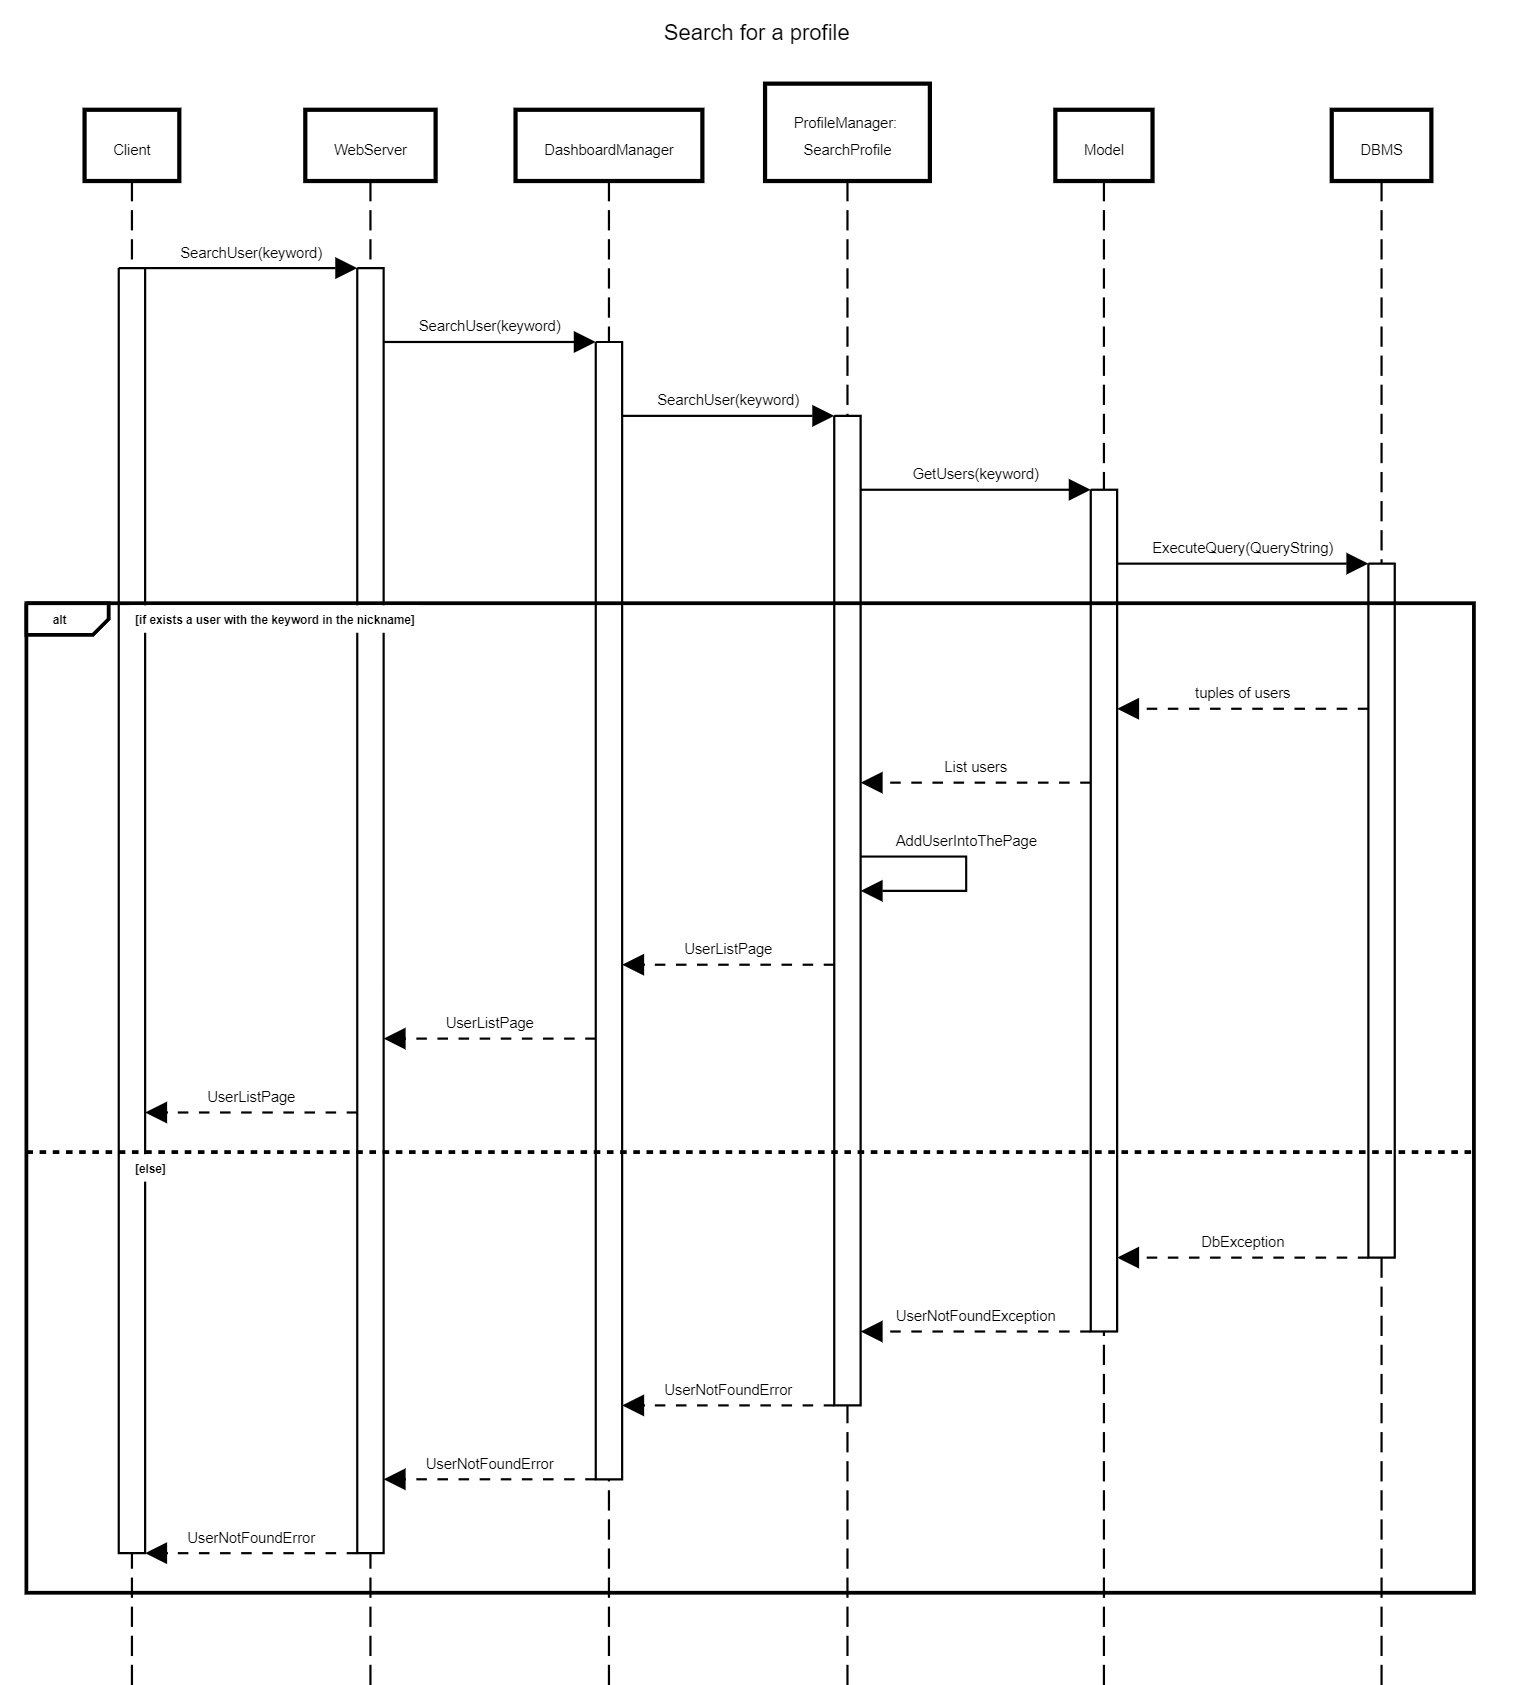
\includegraphics[width=0.8\linewidth]{RuntimeView/SearchProfile.png}
        \caption{Runtime view for 'Search for a profile'.}
        \label{fig:runtime_searchprofile}%
    \end{center}
\end{figure}
This sequence diagram represents the flow behind the profile search.
The User types a keyword into the search bar and sends it to the DashBoardManager that redirects the request to the SearchProfile module.
The SearchProfile module retrieves from the DBMS the list of Users that corresponds to the searched keyword and, if it is not empty, shows it to the User.


\subsection{Search for a Tournament}
\begin{figure}[H]
    \begin{center}
        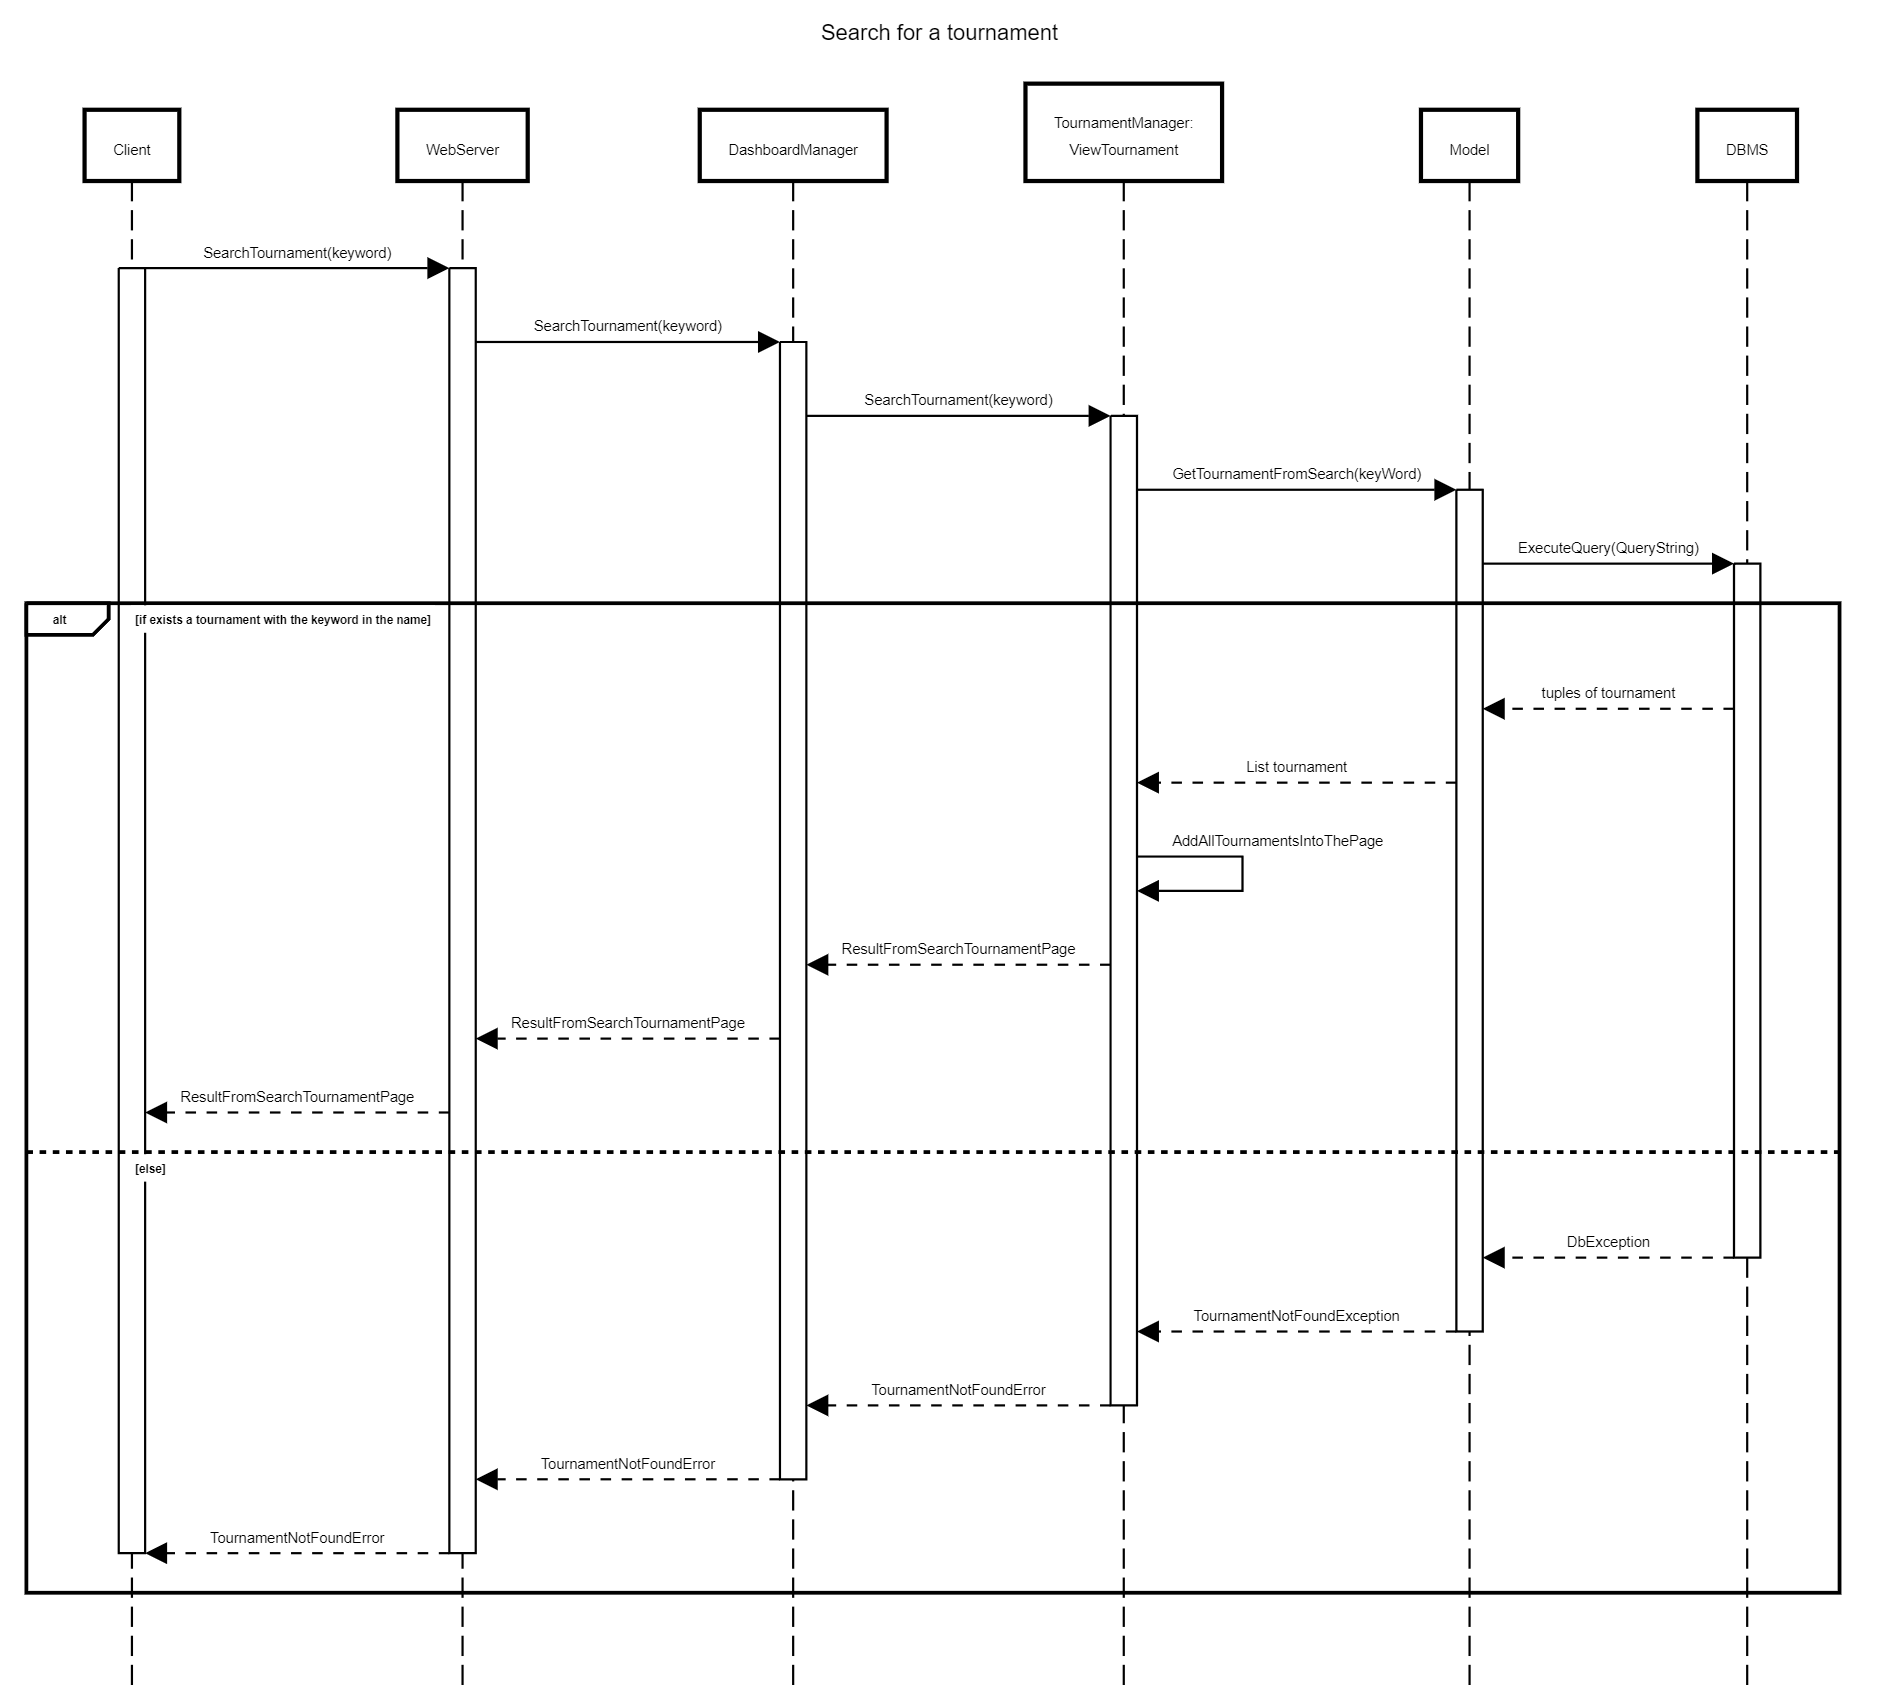
\includegraphics[width=0.8\linewidth]{RuntimeView/SearchTour.png}
        \caption{Runtime view for 'Search for a Tournament'.}
        \label{fig:runtime_searchtournament}%
    \end{center}
\end{figure}
This sequence diagram represents the flow behind the Tournament search.
The User types a keyword into the search bar and sends it to the DashBoardManager that redirects the request to the ViewTournament module.
The ViewTournament module retrieves from the DBMS the list of Tournaments that corresponds to the searched keyword and, if it is not empty, shows it to the User.

\subsection{Evaluate a Code}
\begin{figure}[H]
    \begin{center}
        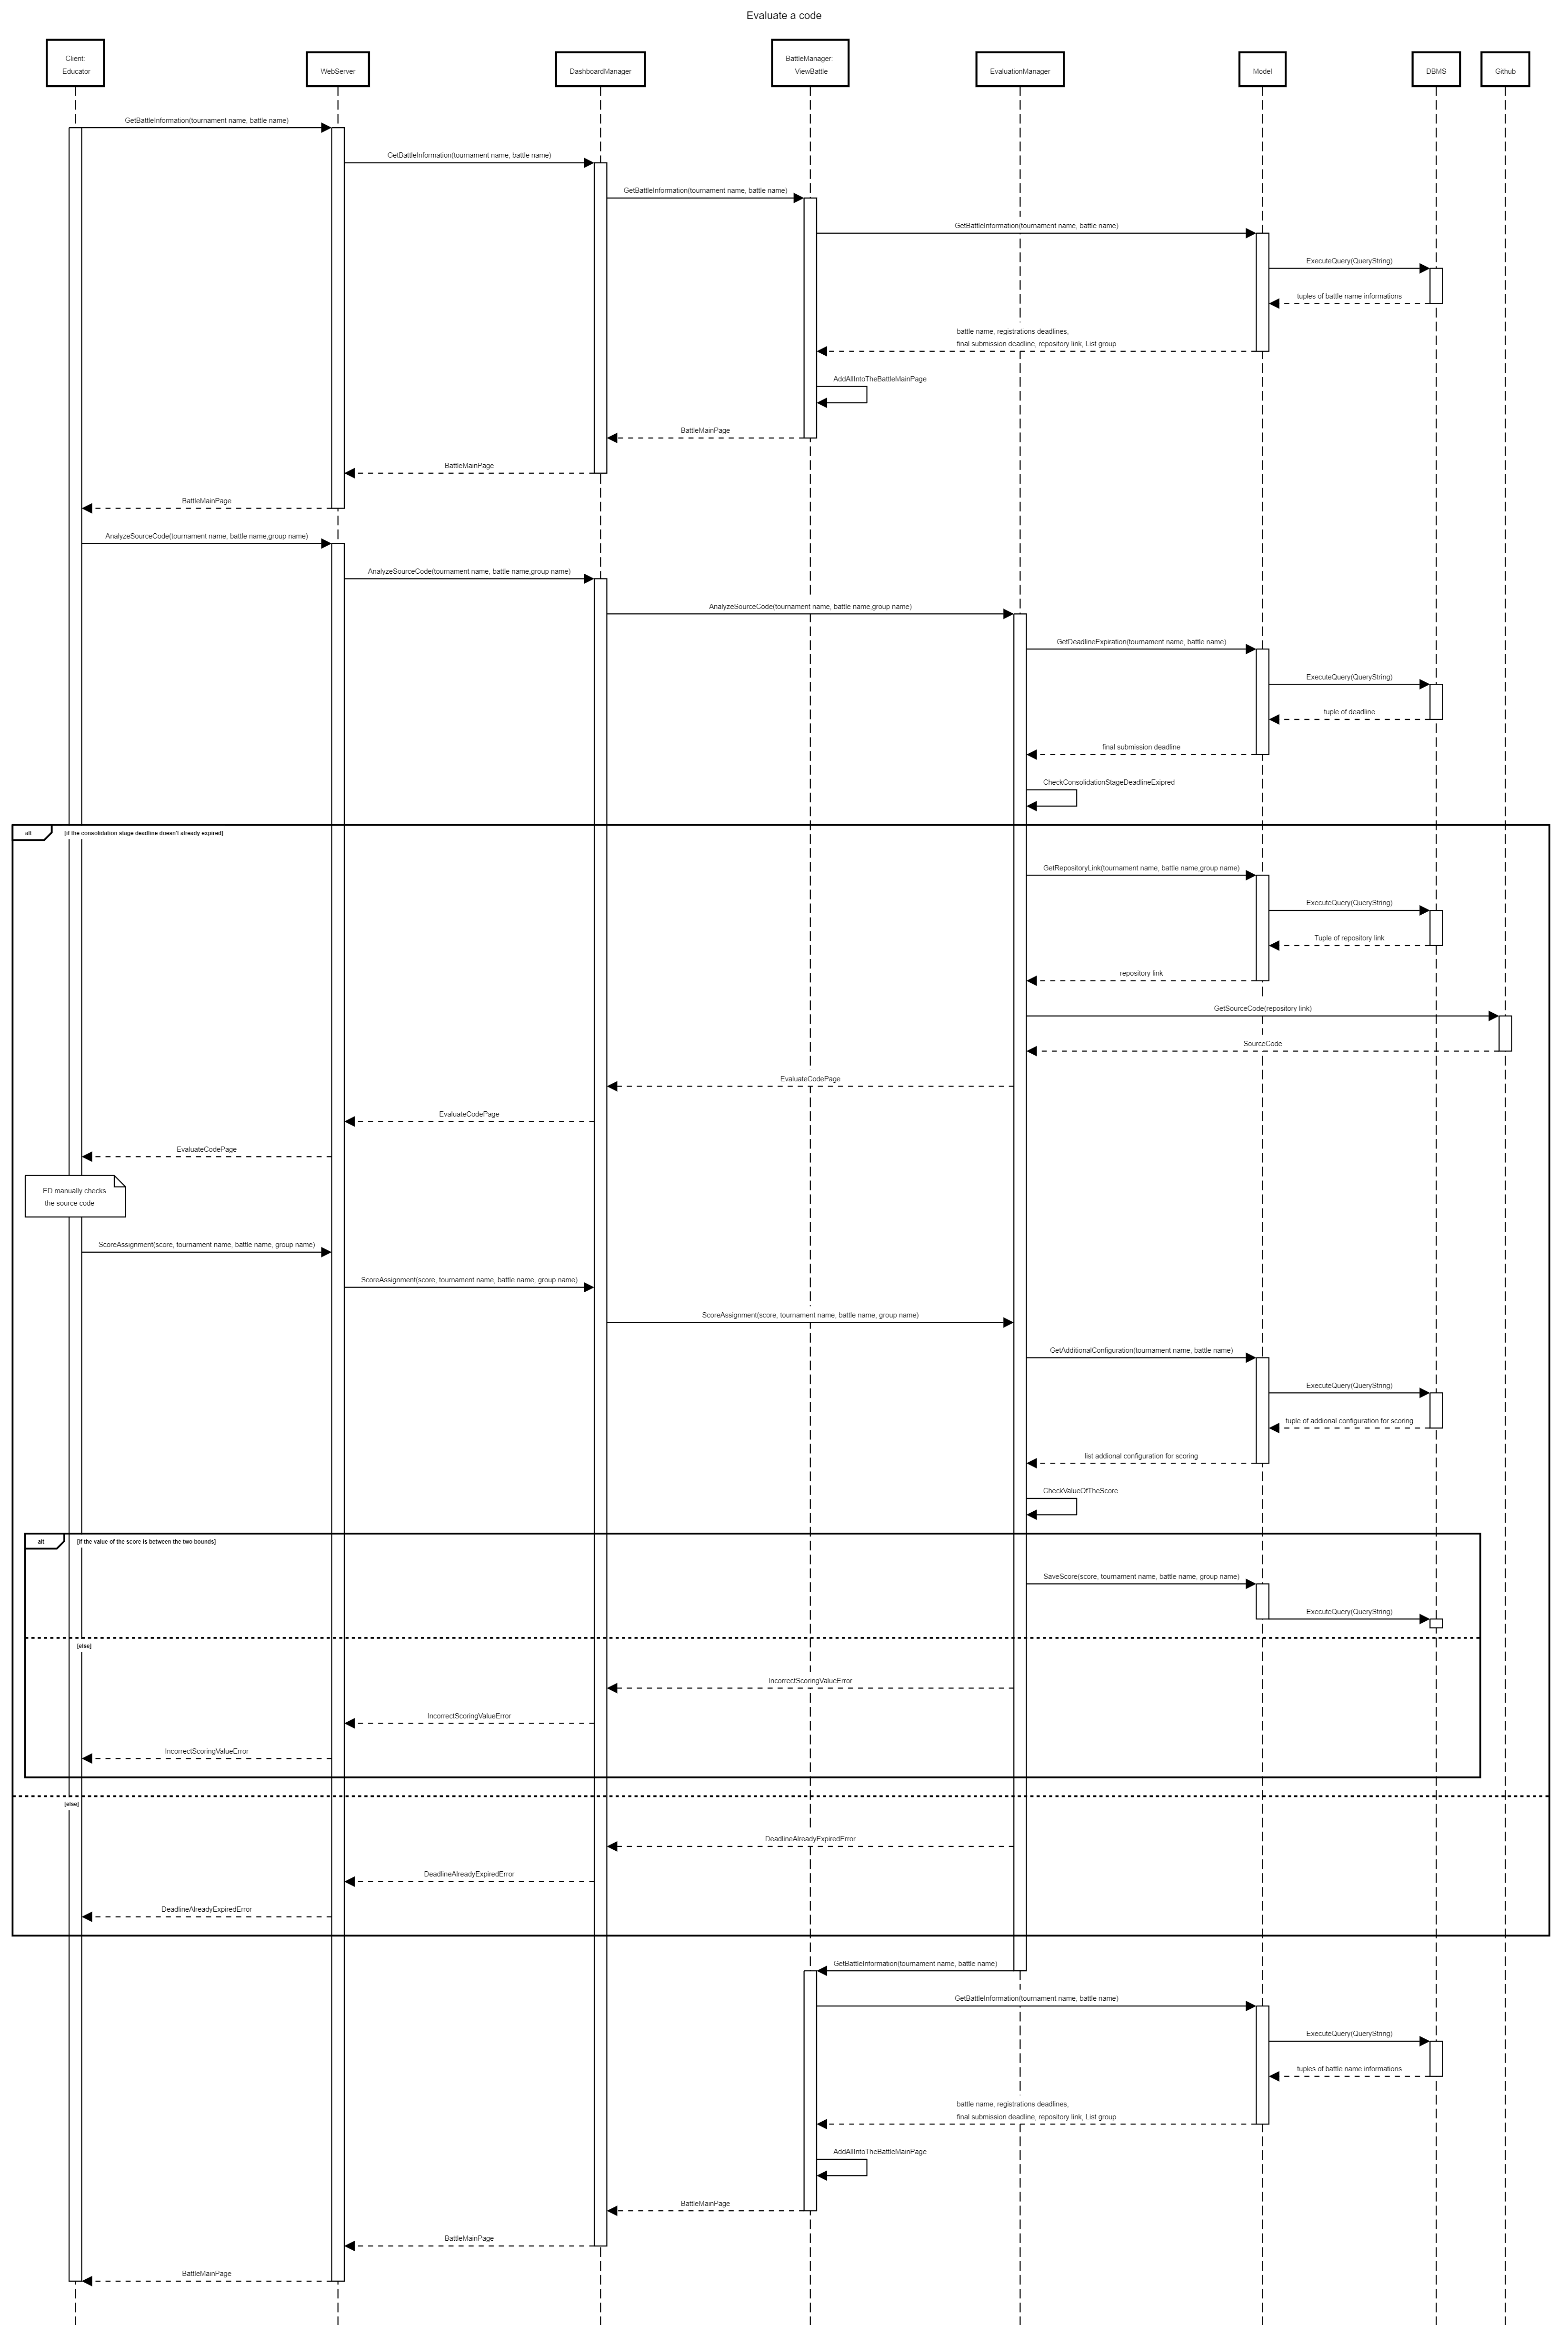
\includegraphics[width=0.8\linewidth]{RuntimeView/EvaluateCode.png}
        \caption{Runtime view for 'Evaluate Code'.}
        \label{fig:runtime_evaluatecode}%
    \end{center}
\end{figure}
This sequence diagram represents the flow behind the ED code evaluation.
The ED clicks on a STG into the ED Battle page and sends his request to the EvaluateManger. The EvaluateManager retrieves the code of that group from GitHub and shows it to the ED. The ED assigns a score to the code and sends it to the EvaluateManger. Finally, the EvaluateManger saves into the Database the score of the STG.

\subsection{Create a new Badge}
\begin{figure}[H]
    \begin{center}
        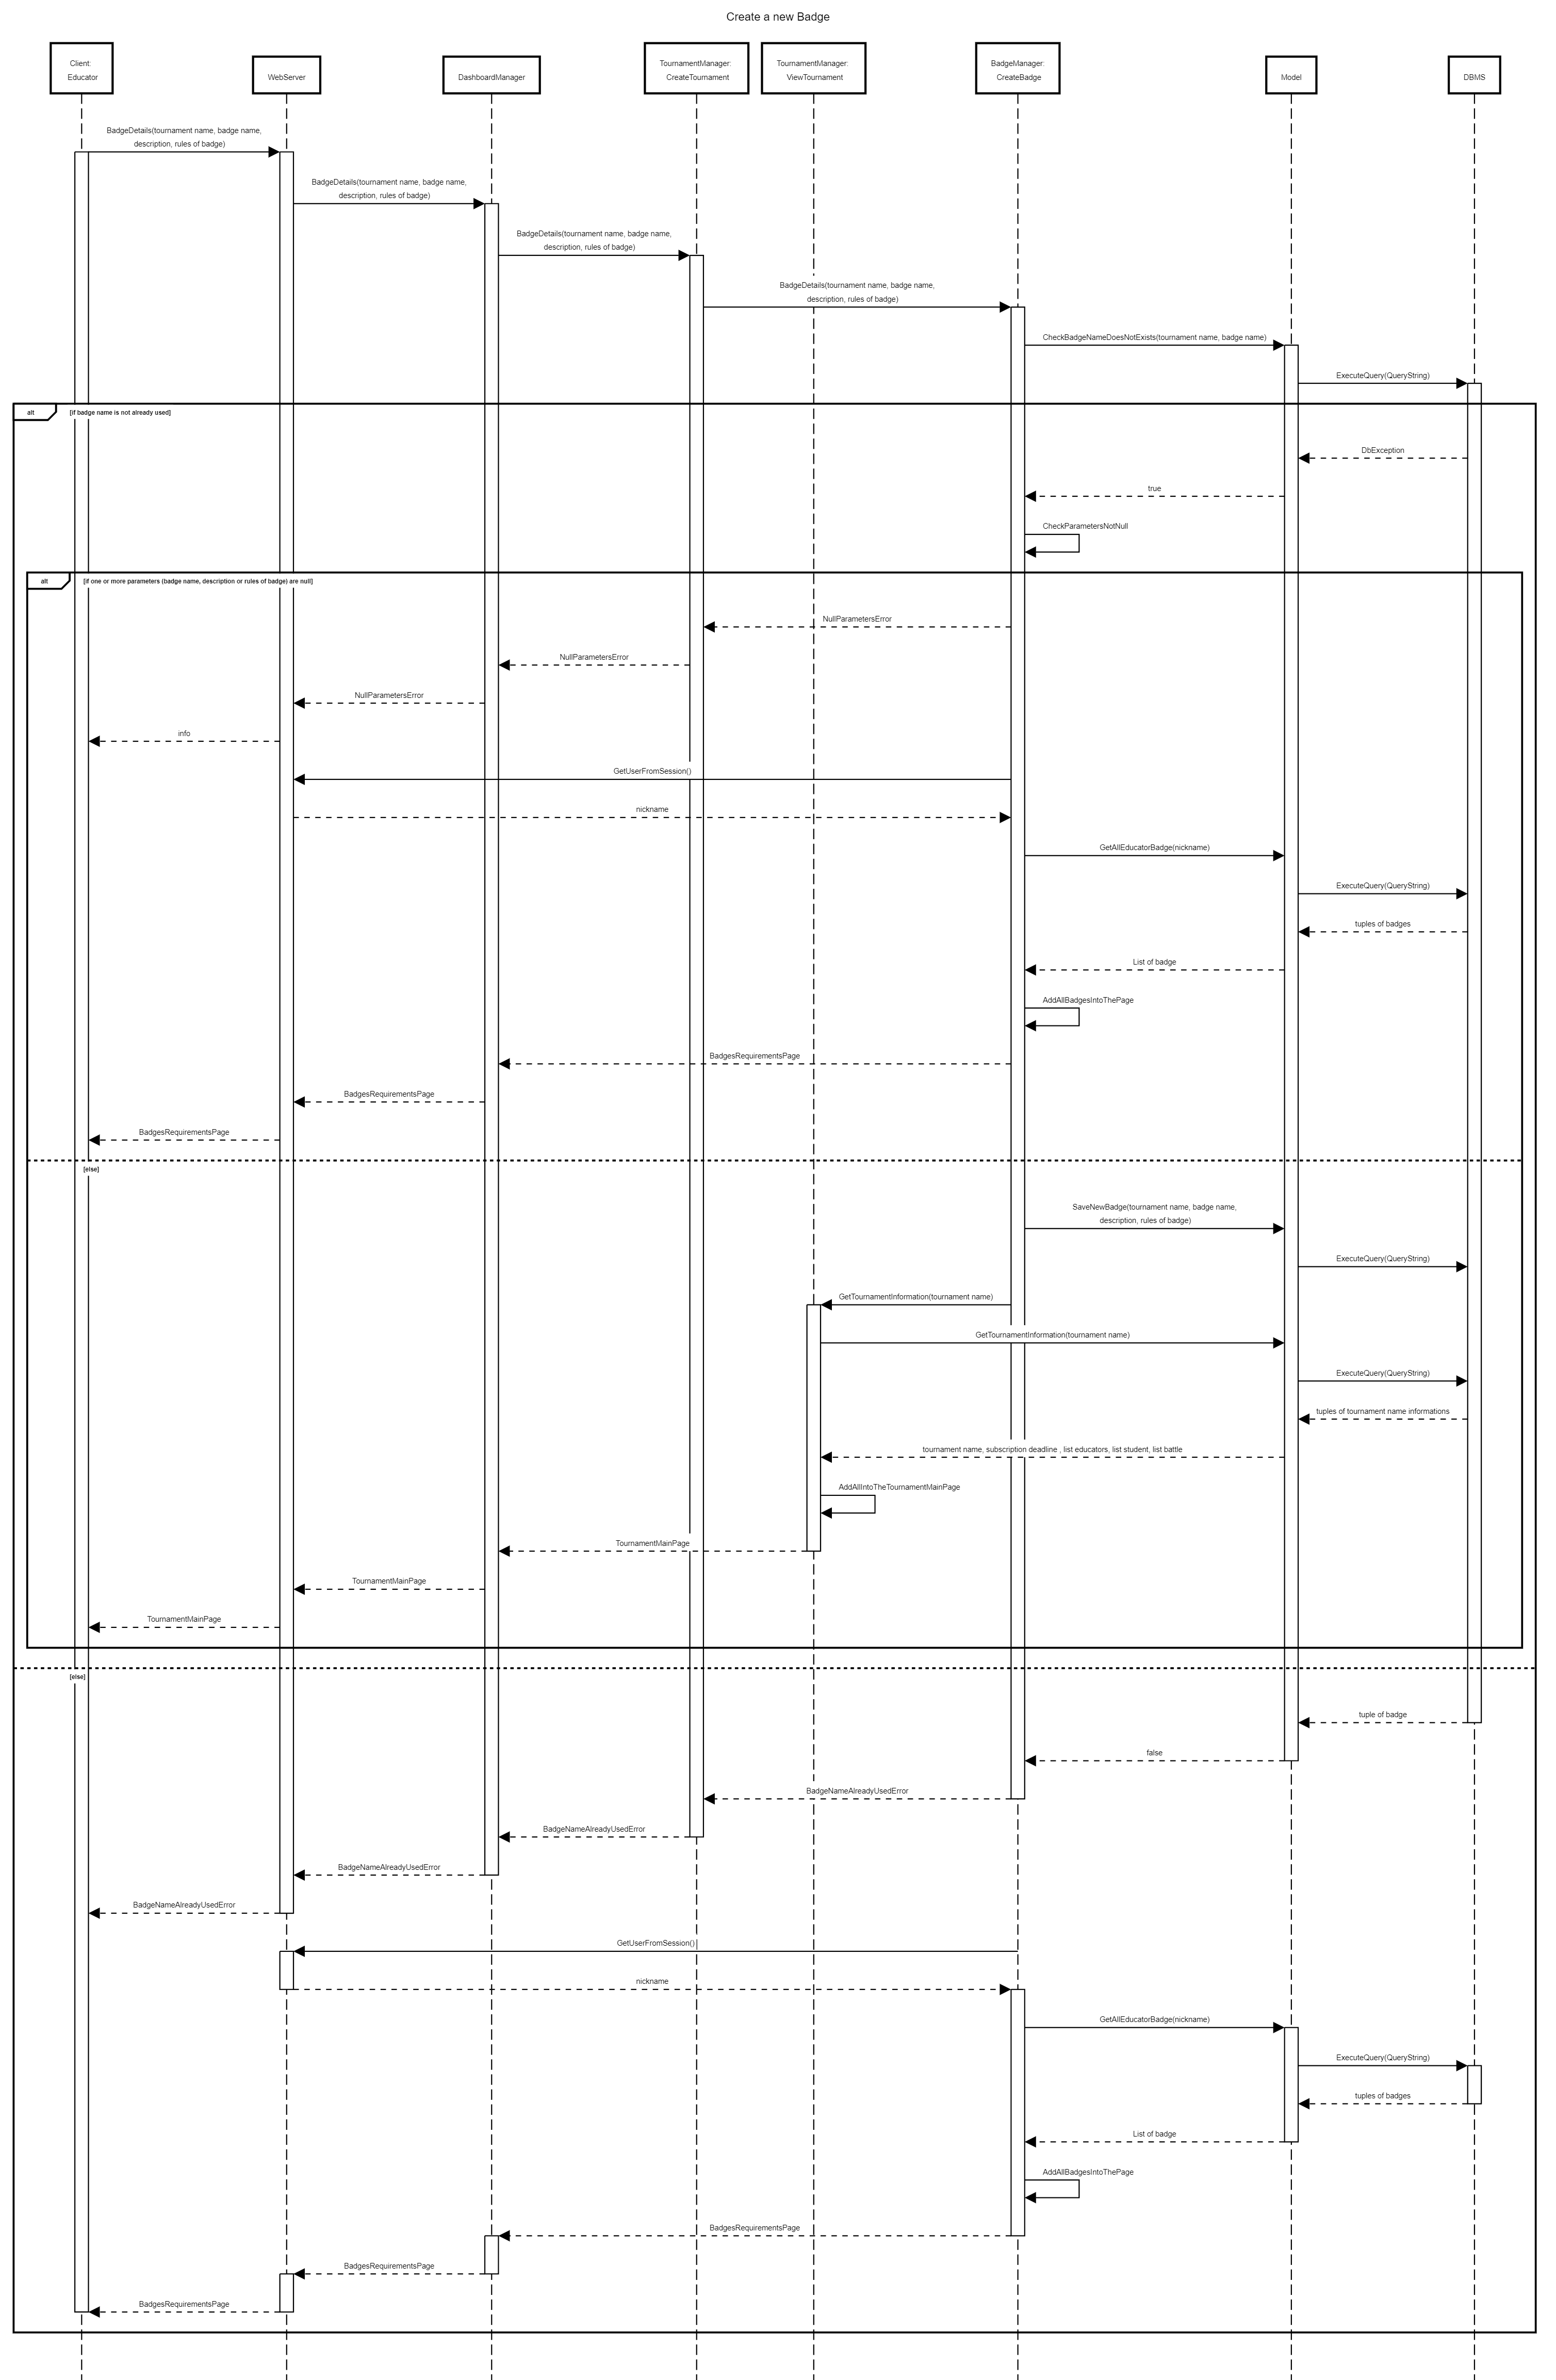
\includegraphics[width=0.8\linewidth]{RuntimeView/CreateBadge.png}
        \caption{Runtime view for 'Create a new Badge'.}
        \label{fig:runtime_createbadge}%
    \end{center}
\end{figure}
This sequence diagram represents the flow behind the creation of a new Badge. The ED inserts into the Create Badge form the information about a new Badge (such as Badge name, description, rules and variables of the Badge) and sends it to the CreateTournament module, which redirects the request to the CreateBadge module. The CreateBadge module checks the new Badge setup and, if they are all correct, saves them into the Database and then calls the ViewTournament module will show the Tournament main page to the ED.

\subsection{Modify an existing Badge}
\begin{figure}[H]
    \begin{center}
        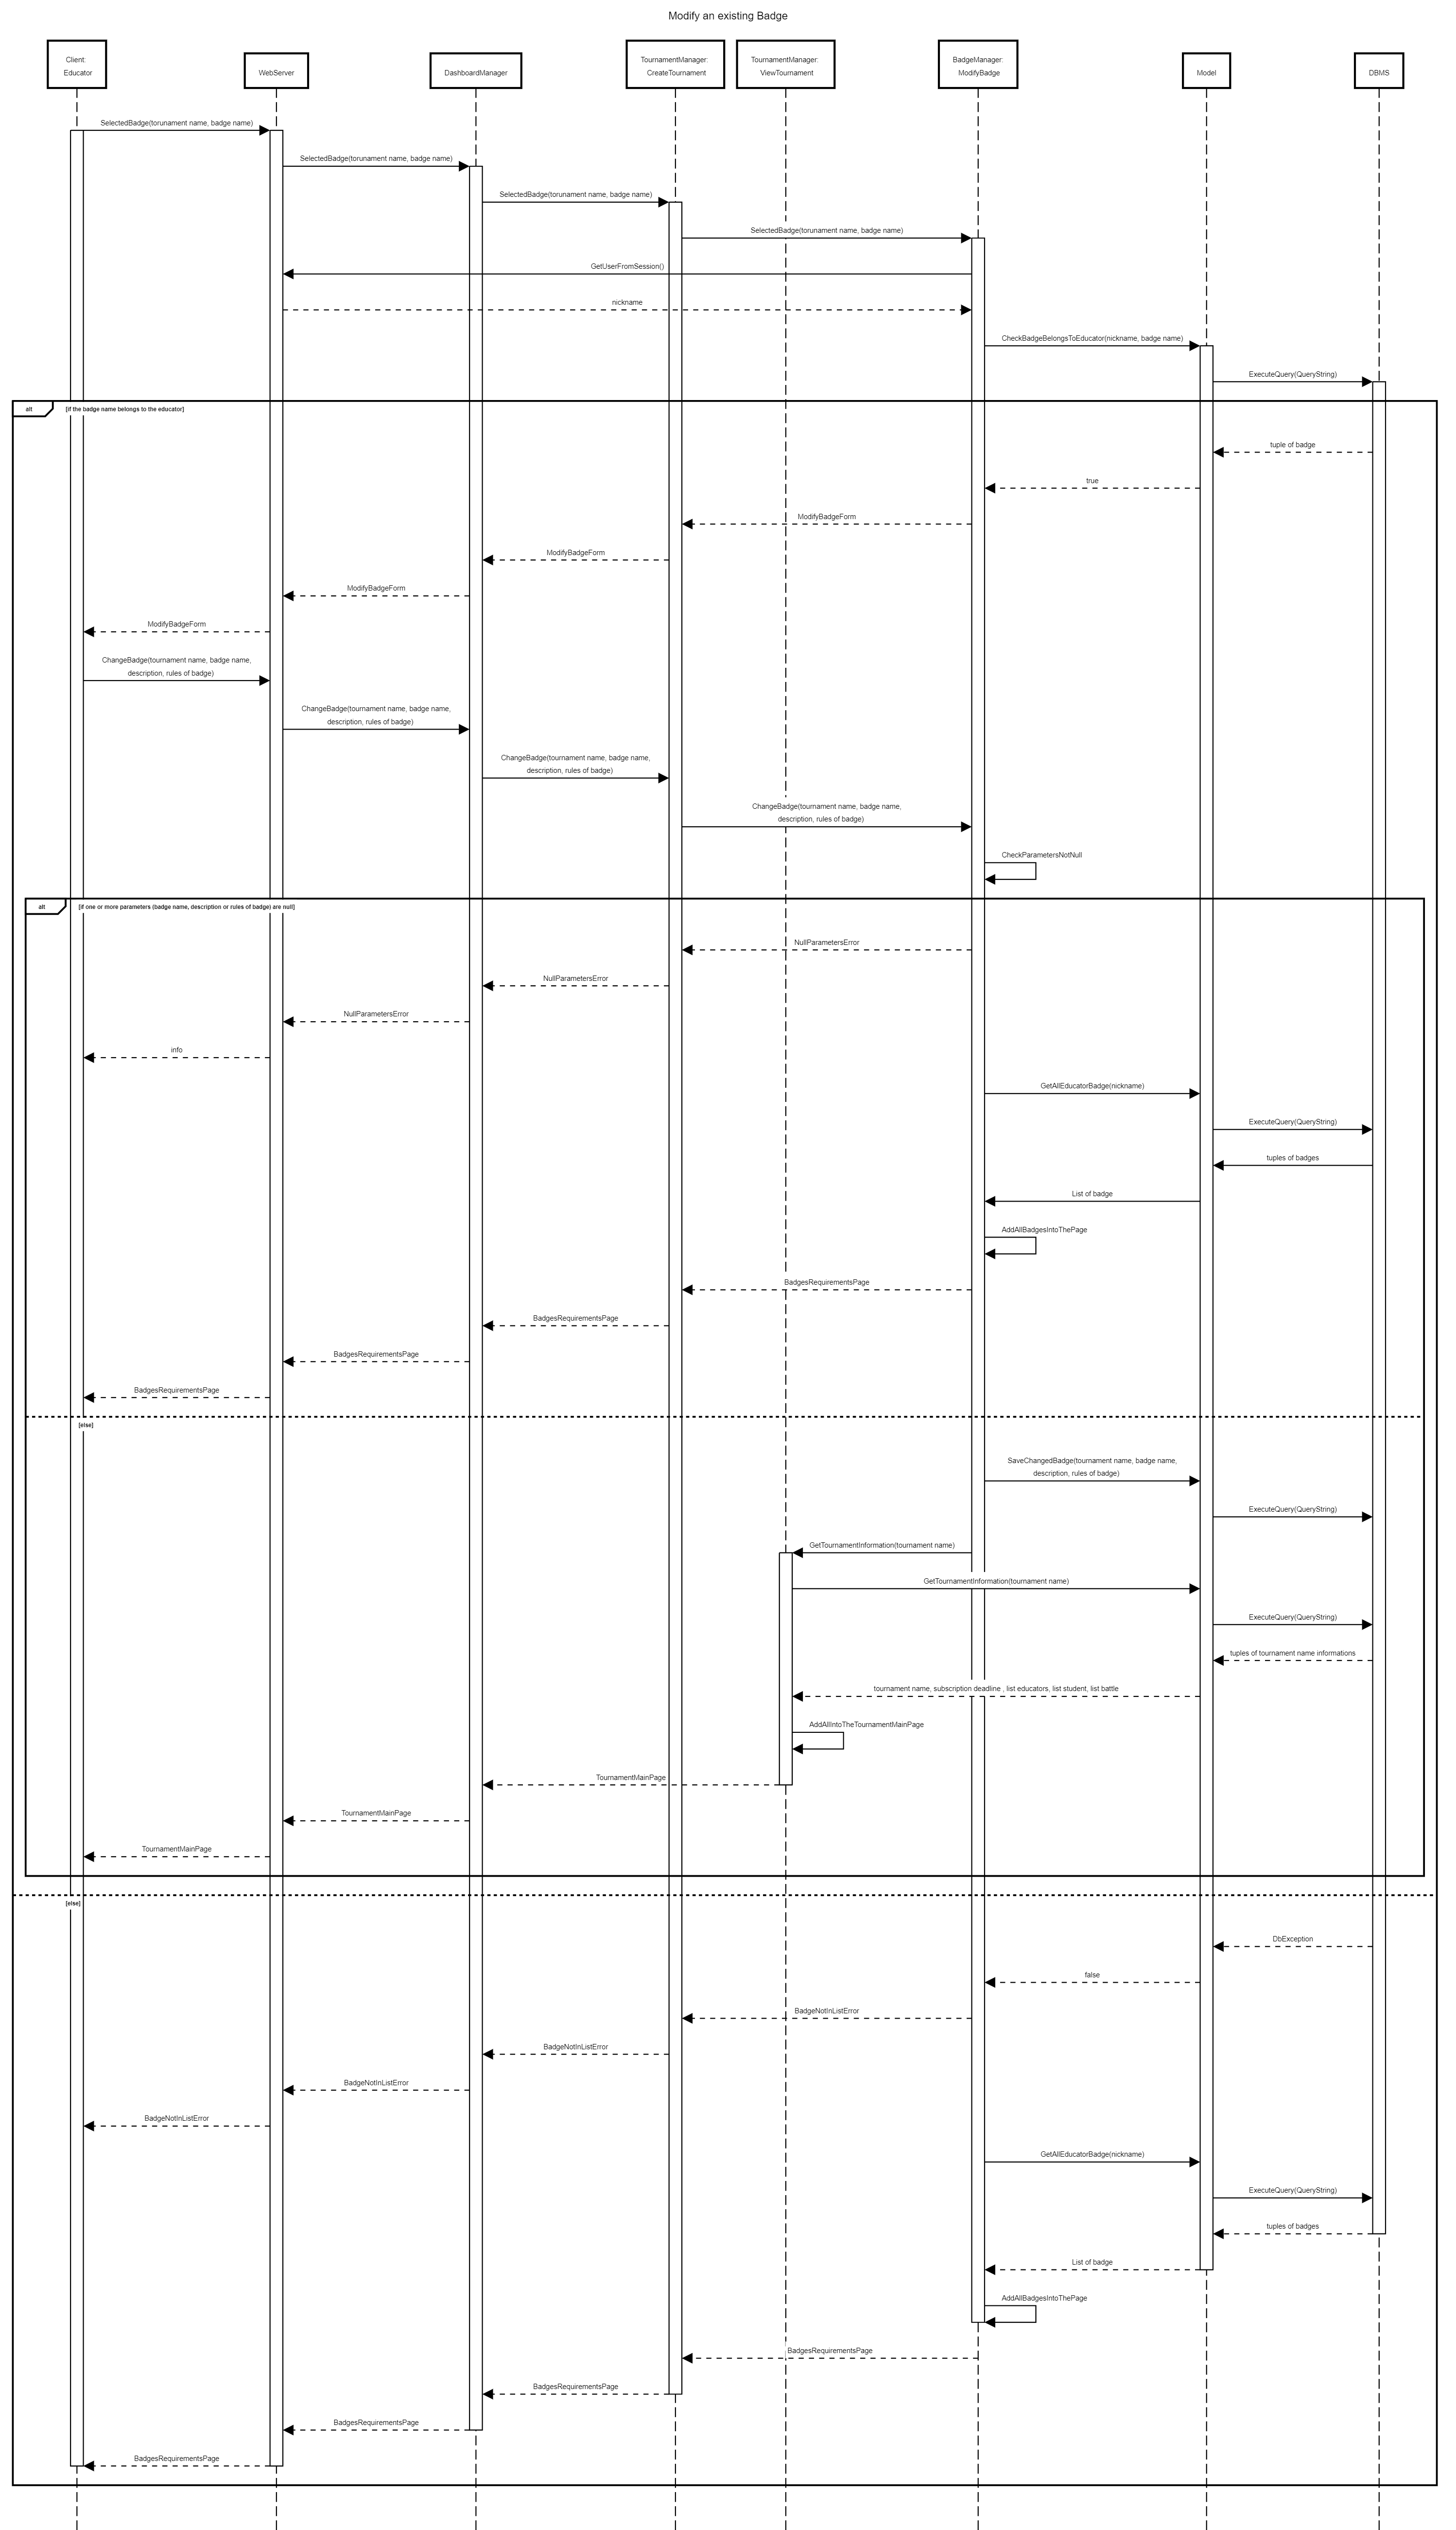
\includegraphics[width=0.8\linewidth]{RuntimeView/ModifyBadge.png}
        \caption{Runtime view for 'Modify an existing Badge'.}
        \label{fig:runtime_modifybadge}%
    \end{center}
\end{figure}
This sequence diagram represents the flow behind the modification of an existing Badge. The ED clicks on an already existing Badge and sends it to the CreateTournament module that redirects the request to the ModifyBadge module that gives to the ED the possibility of changing the badge variables and rules. The ED inserts into the Modify Badge form the new information about the Badge (such as description, rules and variables of the Badge) and sends it to the CreateTournament module, which redirects the request to the ModifyBadge module. The ModifyBadge module checks the new Badge setup and, if they are all correct, saves them into the Database and then calls the ViewTournament module will show the Tournament main page to the ED.





\section{Component Interfaces}
\label{sec:component_interfaces}%
\begin{itemize}
    \item \textbf{\textbf{Login}}
    \begin{itemize}

\item Login(\textit{String} nickname, \textit{String} password)
\end{itemize}
    \item \textbf{\textbf{SearchProfile}}


    \begin{itemize}

\item SearchUser(\textit{String} keyword)
\end{itemize}


    \item \textbf{\textbf{OpenProfile}}
    \begin{itemize}

\item SelectUser(\textit{String} nickname)

\end{itemize}


    \item \textbf{\textbf{RegistrationManager}}

\begin{itemize}
        \item CreateAnAccount()
        \item Registration(\textit{String} name, \textit{String} surname, \textit{String} nickname, \textit{String} mail, \textit{String} password, \textit{Boolean}  ED tick)
        \item Registration(\textit{String} name, \textit{String} surname, \textit{String} nickname, \textit{String} mail, \textit{String} password)
\end{itemize}

    \item \textbf{\textbf{Create Tournament}}

\begin{itemize}
        \item CreateATournament()
        \item TournamentInformation(\textit{String} tournament name, \textit{Date} subscription deadline, \textit{List\textless Educator\textgreater}  list of educators, \textit{Boolean} create badge tick)
        \item BadgeDetails(\textit{String} tournament name, \textit{String} badge name, \textit{String} description, \textit{String} rules of badge)
        \item SelectedBadge(\textit{String} tournament name, \textit{String} badge name)
        \item ChangeBadge(\textit{String} tournament name, \textit{String} badge name, \textit{String} description, \textit{String} rules of badge)
\end{itemize}

    \item \textbf{\textbf{Join Tournament}}
\begin{itemize}
        \item JoinTournament(\textit{String} tournament name)
\end{itemize}

    \item \textbf{\textbf{View Tournament}}

\begin{itemize}
        \item GetTournamentInformation(\textit{String} tournament name)
        \item SearchTournament(\textit{String} keyword)
\end{itemize}

    \item \textbf{\textbf{CreateBadge}}
\begin{itemize}

    \item BadgeDetails(\textit{String} tournament name, \textit{String} badge name, \textit{String} description, \textit{String} rules of badge)
\end{itemize}

    \item \textbf{\textbf{ModifyBadge}}

\begin{itemize}
        \item SelectedBadge(\textit{String} tournament name, \textit{String} badge name)
        \item ChangeBadge(\textit{String} tournament name, \textit{String} badge name, \textit{String} description, \textit{String} rules of badge)
\end{itemize}

    \item \textbf{\textbf{Model}}

\begin{itemize}
        \item CheckCredentials(\textit{String} nickname, \textit{String} password)
        \item GetEducatorTournaments(\textit{String} nickname)
        \item GetStudentTournaments(\textit{String} nickname)
        \item GetNewBattlesFromTournaments(\textit{List\textless Tournament\textgreater} list tournament, \textit{String} nickname)
        \item GetLastTournaments()
        \item GetRepositoryLink(\textit{String} tournament name, \textit{String} battle name, \textit{String} group name)
        \item GetAdditionalConfiguration(\textit{String} tournament name, \textit{String} battle name)
        \item SaveScore(\textit{Int}  score, \textit{String} tournament name, \textit{String} battle name, \textit{String} group name)
        \item CheckNickname(\textit{String} nickname)
        \item CheckMail(\textit{String} mail)
        \item SaveNewUserCredentials(\textit{String} name, \textit{String} surname, \textit{String} nickname, \textit{String} mail, \textit{String} password, \textit{Boolean}  ED tick)
        \item GetAllStudents()
        \item GetUser(\textit{String} nickname)
        \item GetUsers(\textit{String} keyword)
        \item GetDeadlineExpiration(\textit{String} tournament name)
        \item GetDeadlineExpiration(\textit{String} tournament name, \textit{String} battle name)
        \item GetRegistrationDeadline(\textit{String} tournament name, \textit{String} battle name)
        \item CheckBadgeNameDoesNotExists(\textit{String} tournament name, \textit{String} badge name)
        \item GetAllEducatorBadge(\textit{String} nickname)
        \item SaveNewBadge(\textit{String} tournament name, \textit{String} badge name, \textit{String} description, \textit{String} rules of badge)
        \item CheckBadgeBelongsToEducator(\textit{String} nickname, \textit{String} badge name)
        \item SaveChangedBadge(\textit{String} tournament name, \textit{String} badge name, \textit{String} description, \textit{String} rules of badge)
        \item GetTournamentName(\textit{String} tournament name)
        \item GetTournamentInformation(\textit{String} tournament name)
        \item GetTournamentFromSearch(\textit{String} keyWord)
        \item GetStudentTournaments(\textit{String} nickname)
        \item GetLastTournaments()
        \item SaveStudentAsTournamentPartecipant(\textit{String} tournament name, \textit{String} nickname)
        \item GetAllStudentsIntheTournament(\textit{String} tournament name)
        \item CheckStudentAlreadyJoinedTournament(\textit{String} tournament name, \textit{List\textless String\textgreater} list nicknames)
        \item CheckStudentAlreadyJoinedTouenament(\textit{String} tournament name, \textit{String} nickname)
        \item CheckGroupAlreadyJoined(\textit{String} tournament name, \textit{String} battle name, \textit{String} group name)
        \item CheckGroupNumber(\textit{String} tournament name, \textit{String} battle name, \textit{String} group name)
        \item SaveGroupIntheBattleList(\textit{String} tournament name, \textit{String} battle name, \textit{String} group name)
        \item CheckBattleName(\textit{String} tournament name, \textit{String} battle name)
        \item GetBattleInformation(\textit{String} tournament name, \textit{String} battle name)
        \item CheckGroupName(\textit{String} tournament name, \textit{String} battle name, \textit{String} group name)
        \item CheckGroupParticipants(\textit{String} tournament name, \textit{String} battle name, \textit{String} group name)
        \item AddStudentToGroup(\textit{String} nickname, \textit{String} tournament name, \textit{String} battle name, \textit{String} group name)
        \item CreateNewBattle(\textit{String} tournament name, \textit{String} battle name, \textit{String} code kata, \textit{Int}  minimum member per group, \textit{Int}  maximum member per group, \textit{Date} registration deadline, \textit{Date} final submission deadline, \textit{List\textless String\textgreater} list additional configuration for scoring, \textit{String} repository link)
        \item CheckStudentAlreadyJoinedBattle(\textit{String} battle name, \textit{String} tournament name, \textit{String} nickname)
        \item GetEducatorsName(\textit{List\textless Educators\textgreater} list of educators)
        \item SaveNewTournament(\textit{String} tournament name, \textit{String} subscription deadline, \textit{List\textless Educators\textgreater} list of educators)
\end{itemize}

    \item \textbf{\textbf{CreateBattle}}

\begin{itemize}
        \item NewBattle(\textit{String} tournament name)
        \item CreateBattle(\textit{String} battle name, \textit{String} code kata, \textit{Int}  minimum member per group, \textit{Int}  maximum member per group, \textit{Date} registration deadline, \textit{Date} final submission deadline, \textit{List\textless String\textgreater} list additional configuration for scoring)
\end{itemize}

\end{itemize}

\begin{itemize}
    \item \textbf{\textbf{JoinBattle}}
\begin{itemize}
    \item ChooseBattle(\textit{String} tournament name, \textit{String} battle name)
    \end{itemize}


    \item \textbf{\textbf{CreateGroup}}

\begin{itemize}
        \item CreateGroupAndInvitation(\textit{String} tournament name, \textit{String} battle name, \textit{String} group name, \textit{List\textless String\textgreater} list nicknames)
        \item acceptInvitation(Student student, \textit{String} tournament name, \textit{String} battle name, \textit{String} group name)
        \item rejectInvitation(Student student, \textit{String} tournament name, \textit{String} battle name, \textit{String} group name)
        \item JoinBattle(\textit{String} tournament name, \textit{String} battle name, \textit{String} group name)
\end{itemize}

    \item \textbf{\textbf{ViewBattle}}
    \begin{itemize}
        \item GetBattleInformation(\textit{String} tournament name, \textit{String} battle name)
\end{itemize}

    \item \textbf{\textbf{EndBattle}}
\begin{itemize}
        \item StartFinalBattleTimer(\textit{String} tournament name, \textit{String} battle name, \textit{Date} final submission deadline)
\end{itemize}

    \item \textbf{\textbf{NotificationManager}}

\begin{itemize}
        \item ChosenEducatorNotification(\textit{String} nickname, \textit{String} tournament name)
        \item NewBattleNotification(\textit{String} nickname, \textit{String} tournament name, \textit{String} battle name)
        \item NewTournamentNotification(\textit{String} nickname, \textit{String} tournament name)
        \item SendInvitation(\textit{String} nickname, \textit{String} tournament name, \textit{String} battle name, \textit{String} group name)
\end{itemize}

    \item \textbf{\textbf{EvaluationManager}}

\begin{itemize}
        \item AnalyzeSourceCode(\textit{String} tournament name, \textit{String} battle name, \textit{String} group name)
        \item ScoreAssignment(\textit{Int}  score, \textit{String} tournament name, \textit{String} battle name, \textit{String} group name)
\end{itemize}

    \item \textbf{\textbf{DashboardManager}} (contains all the interfaces belonging to other managers, apart from NotificationManager and Model)

    \item \textbf{\textbf{WebServer}} (contains all the interfaces belonging to other managers, apart from NotificationManager and Model)
    \begin{itemize}
        \item GetSessionFromUser()
        \item AddUserToTheSession(\textit{String} nickname, \textit{String} password)
\end{itemize}

\end{itemize}


\section{Selected Architectural Styles and Patterns}
\label{sec:selected_Srchitectural_styles_patterns}%

CodeKataBattle will be developed over a \textbf{3-Tier architecture}, which is a software application architecture that organizes applications into three logical and physical computing tiers. Each tier runs on its own infrastructure, so the complexity of the system is reduced, its flexibility and scalability is enhanced. Each tier may be developed simultaneously by separate teams of developers and can be updated or scaled as needed without impacting the other tiers.
\\
The system is modularized over three independent tiers:
\begin{itemize}
    \item \textbf{Presentation Tier:} this is the top-level tier, that directly interacts with the Users. Its goal will be to collect the Users’ inputs and show them the outputs produced by the lower tiers. 
    \item \textbf{Application Tier:} this is the middle level tier. The Application Tier processes the Users’ requests that arrive from the Presentation Tier, perform the necessary computation, even retrieving or storing data on the Data Tier, and computes that data in order to complete specific tasks requested by the Users. This tier needs to handle several requests by different Users simultaneously, while guaranteeing the security and integrity of the stored data.
    \item \textbf{Data Tier:} this is the lowest level tier. The Data Tier stores, retrieves and manages data used or produced by the Application Tier by the DataBase System’s APIs.
\end{itemize}

For a more detailed description of the tiers and their components, please refer to \ckbautoref{sec:deployment_view}.\\
The behavior of the system will be mostly as a \textbf{Client-Server architecture}, in which the Client represents the front-end user interface, as it is the connection point between the final Users of the system and the system itself, meanwhile the Server represents the backend platform, as it elaborates the Users’ requests, computes and shows the answers. In a pure Client-Server architecture, the Server is always the one to make the request, while the server is a passive element, which handles and elaborates the requests of the Client and returns the answers to them. In some cases, such as when the process of sending the notifications or the interaction with the External Tools, the Server needs to perform operations without being invoked by the Client first, which makes it an active component and having a more Event Driven behavior.
\\
The Client-Server interactions are performed through \textbf{REST APIs}, a set of commands commonly used in the context of web transactions. The \textit{Representational State Transfer} consists in the use of a stateless Server, that means that the Client is the component that needs to communicate the state of the transaction to the Server. This approach allows the Server to be more scalable and helps with handling many requests that concern different states simultaneously. The components communicate by transferring a representation of a resource in a format that the Server is able to process, this allows the usage of HTTP protocol to share data and to encode those using the JSON format.
\\
The implementation of CKB will follow the \textbf{Model-View-Controller} pattern, which is a software design pattern that splits the software into three elements interconnected with each other: 
\begin{itemize}
    \item \textbf{Model:} contains the methods that manage the data. It provides methods for saving, retrieving and manipulating data from the database.
    \item \textbf{View:} the view is the part that concerns the visual representation of the data for the final user.
    \item \textbf{Controller:} acts as a connection point between the view and the model. The controller handles the users’ interactions with the view and processes the operations.
\end{itemize}

\section{Other Design Decisions}
\label{sec:other_design_decisions}%

\subsection{Availability}
The introduction of load balancing and replication mechanisms significantly enhances the reliability and availability of our system. Load balancing optimizes resource utilization by distributing requests evenly across servers, preventing performance bottlenecks.\\ Concurrently, replication ensures fault tolerance by duplicating essential data and services. This redundancy minimizes the impact of potential failures, fortifying our system to maintain consistent data management and service availability even in challenging scenarios.

\subsection{Scalability}
Microservices architecture, at its core, is meticulously crafted to be both independently deployable and inherently scalable. This design philosophy enables each microservice to be deployed autonomously, facilitating swift updates and modifications without disrupting the entire system. Beyond this, the scalability aspect of microservices empowers our system to gracefully handle increased demands by efficiently scaling specific services.


\subsection{Notification Handling}
Notification management plays a pivotal role in the CKB system, influencing every stage from Tournament, Battle or STG creation to their conclusion. Notifications in CKB are orchestrated to reach users upon login or, if a User is already logged in, immediately when they become available. This approach guarantees that Users are promptly informed about key events, such as Tournament, Battle or STG creation. 

\subsection{Ease of Deployment} 
The adoption of microservices architecture introduces a notable advantage in ease of deployment. This methodology empowers the implementation of changes to individual services independently, allowing for seamless deployment without impacting the entire system. In the event of issues, the microservices approach facilitates swift identification, isolation, and correction, eliminating the need to halt the entire system. This deployment flexibility not only accelerates the release of updates but also enhances the system's resilience and agility, enabling efficient troubleshooting and maintenance processes.

\subsection{Data Storage} 
To enhance operational efficiency and simplify data management, we've chosen a unified DBMS containing information about Users, Tournaments, Group, Badges and Battles. This approach reduces the time and complexity associated with retrieving and updating data, leveraging interconnected relationships among these components.


    \chapter{User Interface Design}
    \label{ch:user_interface_design}%
    This section outlines the User Interface of the S\&C system, providing an overview of the various pages that form the core of the platform. The design mockups presented in this document focus on interaction dynamics and functionality rather than the final visual aesthetics, acknowledging that graphical elements may undergo adjustments during the testing and refinement phases. While the desktop browser version is emphasized due to its alignment with the platform's primary objective of connecting students and companies, equivalent pages will be designed and optimized for the mobile version to ensure a seamless and responsive user experience across devices.

As highlighted in the RASD, these design mockups serve as an initial representation of the interface and are subject to iterative enhancements based on testing outcomes and user feedback, ensuring that the system meets the expectations of its target audience while maintaining usability and efficiency.


\section{Overview}

\begin{figure}[H]
    \begin{center}
        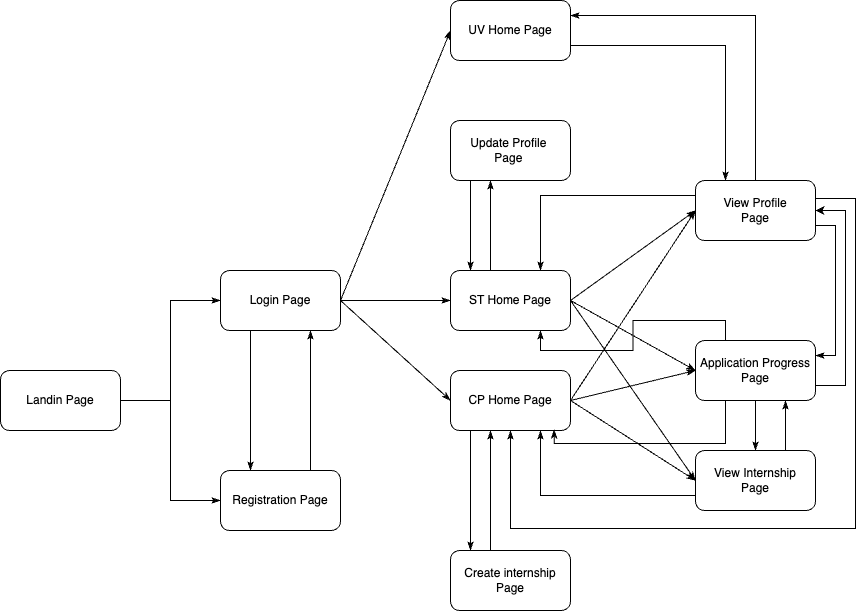
\includegraphics[width=0.8\linewidth]{Interfaces_UI/Overview.png}
        \caption{User Interface Overview.}
        \label{fig:user_interface_overview}%
    \end{center}
\end{figure}

The provided diagram presents a comprehensive overview of the S\&C system’s pages, illustrating their interconnections and the primary pathways for user navigation. Each page serves a specific purpose in enabling seamless interaction between students and companies. Detailed descriptions of each page are provided in the following sections, with the exception of the landing page, which is implicit as it primarily serves as an introduction to the platform and provides access to the login and registration pages.


\section{Header}

\begin{figure}[H]
    \begin{center}
        
\includegraphics[width=1\linewidth]{Interfaces_UI/Header.png}
        \caption{Header.}
        \label{fig:header}%
    \end{center}
\end{figure}

Across all pages in the S\&C system, a uniform header ensures a consistent and user-friendly experience. The header prominently displays the platform name, a notification icon to keep users updated, a menu icon for easy navigation, and the user’s name or identifier. These elements provide quick access to essential features, enhancing usability across the platform.

In cases where the user is a company or a university, the header undergoes slight modifications to better cater to their role. For instance, instead of the user's name, the company or institution’s name is displayed, reflecting their organizational identity. Additionally, the menu options adapt to include functionalities specific to these users, such as "Recommended Students" or "Create Tasks." Despite these changes, the cohesive design of the header remains consistent, ensuring familiarity and accessibility for all users.
 

\newpage

\section{User Interfaces}
\newcounter{ui}
\setcounter{ui}{1}
\newcommand{\cui}{\theui\stepcounter{ui}}

\subsection*{UI\cui . Login and Registration Pages}

\begin{figure}[H]
    \begin{center}
        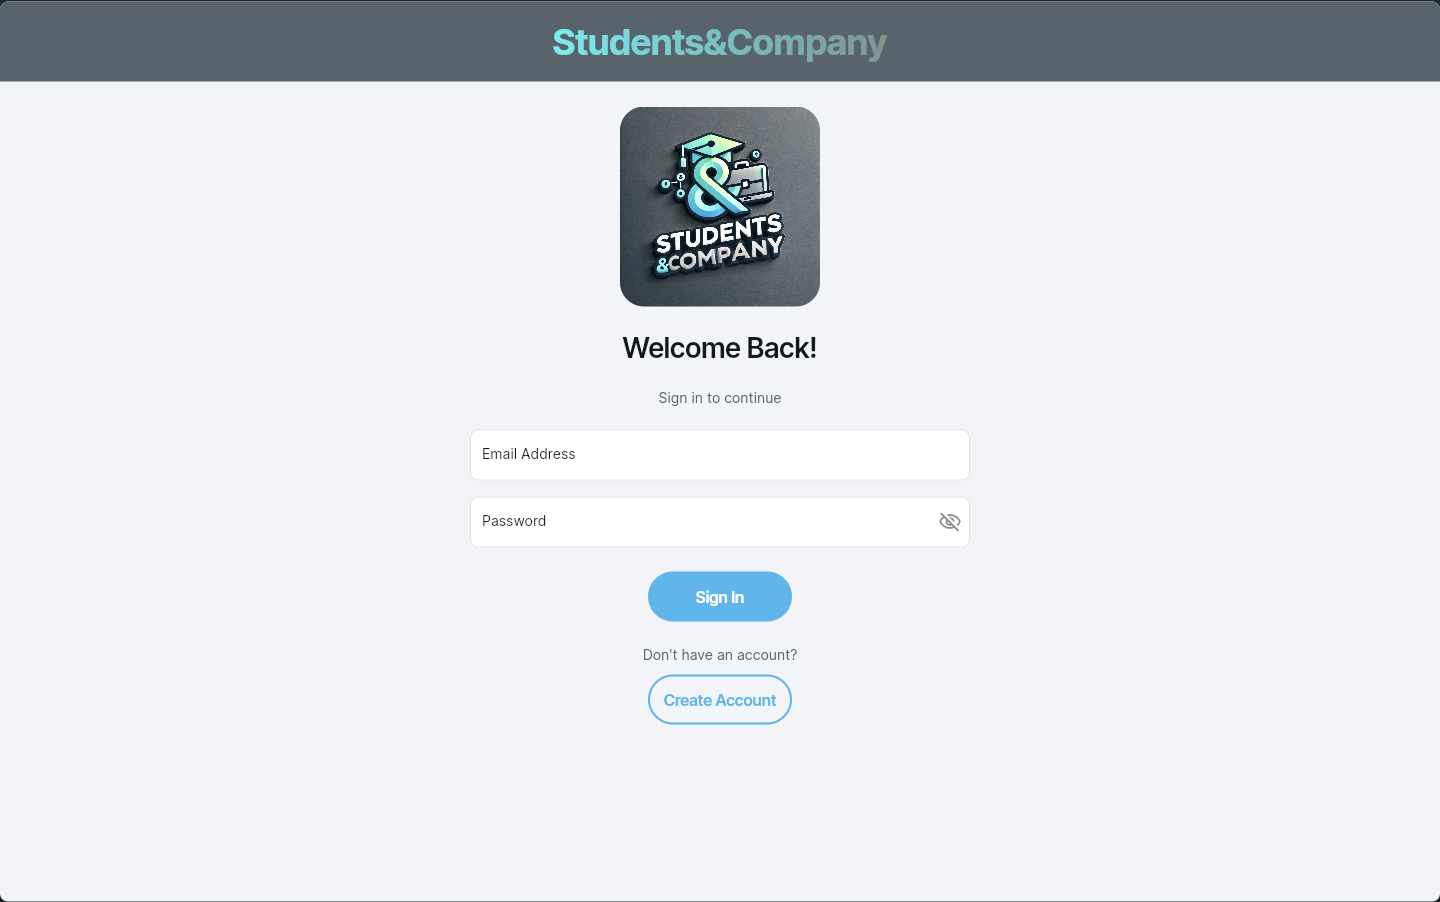
\includegraphics[width=0.7\linewidth]{Interfaces_UI/LoginPage.png}
        \caption{Login Page.}
        \label{fig:login_page}%
    \end{center}

    \begin{center}
        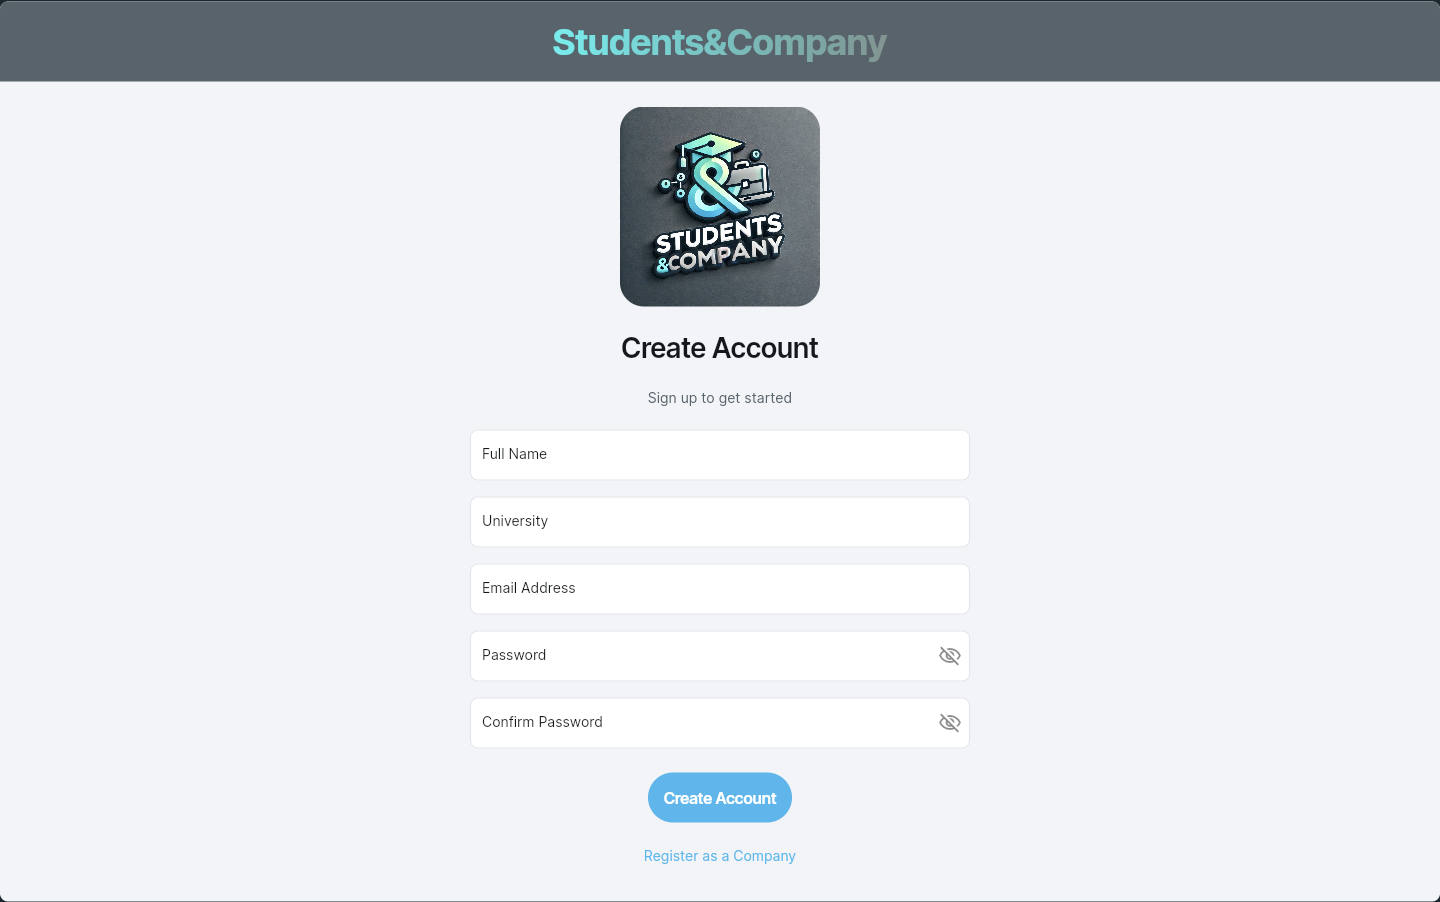
\includegraphics[width=0.7\linewidth]{Interfaces_UI/RegistrationPage.png}
        \caption{Registration Page.}
        \label{fig:registration_page}%
    \end{center}
\end{figure}

The "Login" and "Registration" pages are simple form pages that allow user to register and sign in.  For the Login page, either if the User is a ST or CP or UV, they just need to enter their credentials to login. The registration's steps are a bit different between them, for STs they need to specify their Full name, email, password and the the university they belong to; for both CPs and UVs, they need to specify some other aspects to make sure that not everyone can register as CP or UV.

\subsection*{UI\cui . ST Homepage}

\begin{figure}[H]
    \begin{center}
        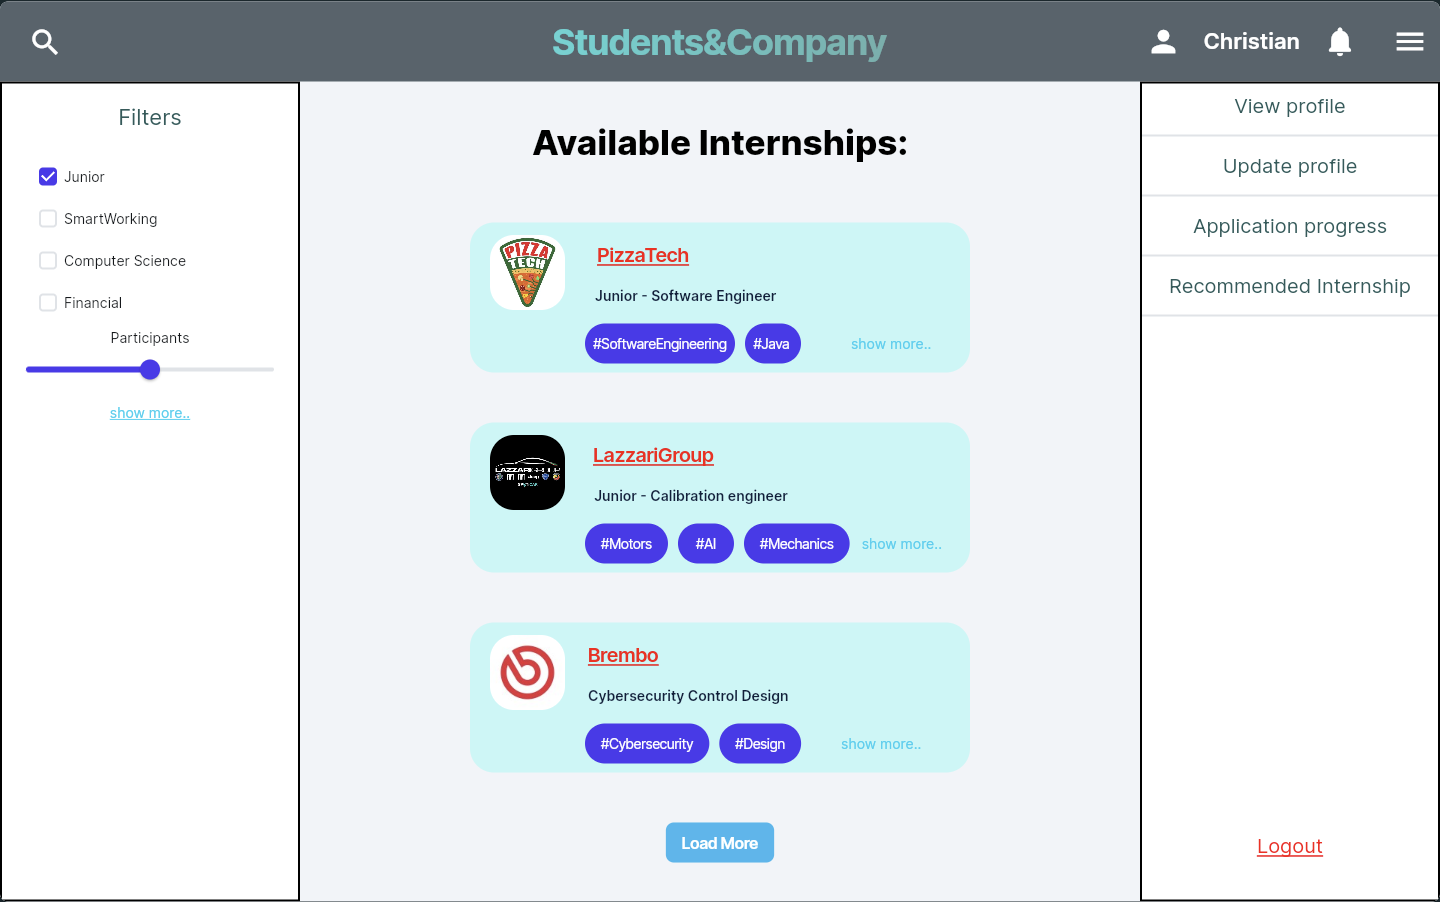
\includegraphics[width=0.7\linewidth]{Interfaces_UI/STHomePage.png}
        \caption{ST Homepage.}
        \label{fig:st_homepage}%
    \end{center}
\end{figure}

From the Login Page, the ST will be redirected to the Student Homepage, which is composed by a scrollable feed of internships in the center. On the left side ST can apply filters for a better search of internships, also with the possibility of a keyword search by writing on the lens at the top. On the right there is a drop-down menu that allows ST to view their profile, update it in the case they have not done it yet, the application progress page that will be explained later, and the possibility to Logout.

\subsection*{UI\cui . Update Profile Page}

\begin{figure}[H]
    \begin{center}
        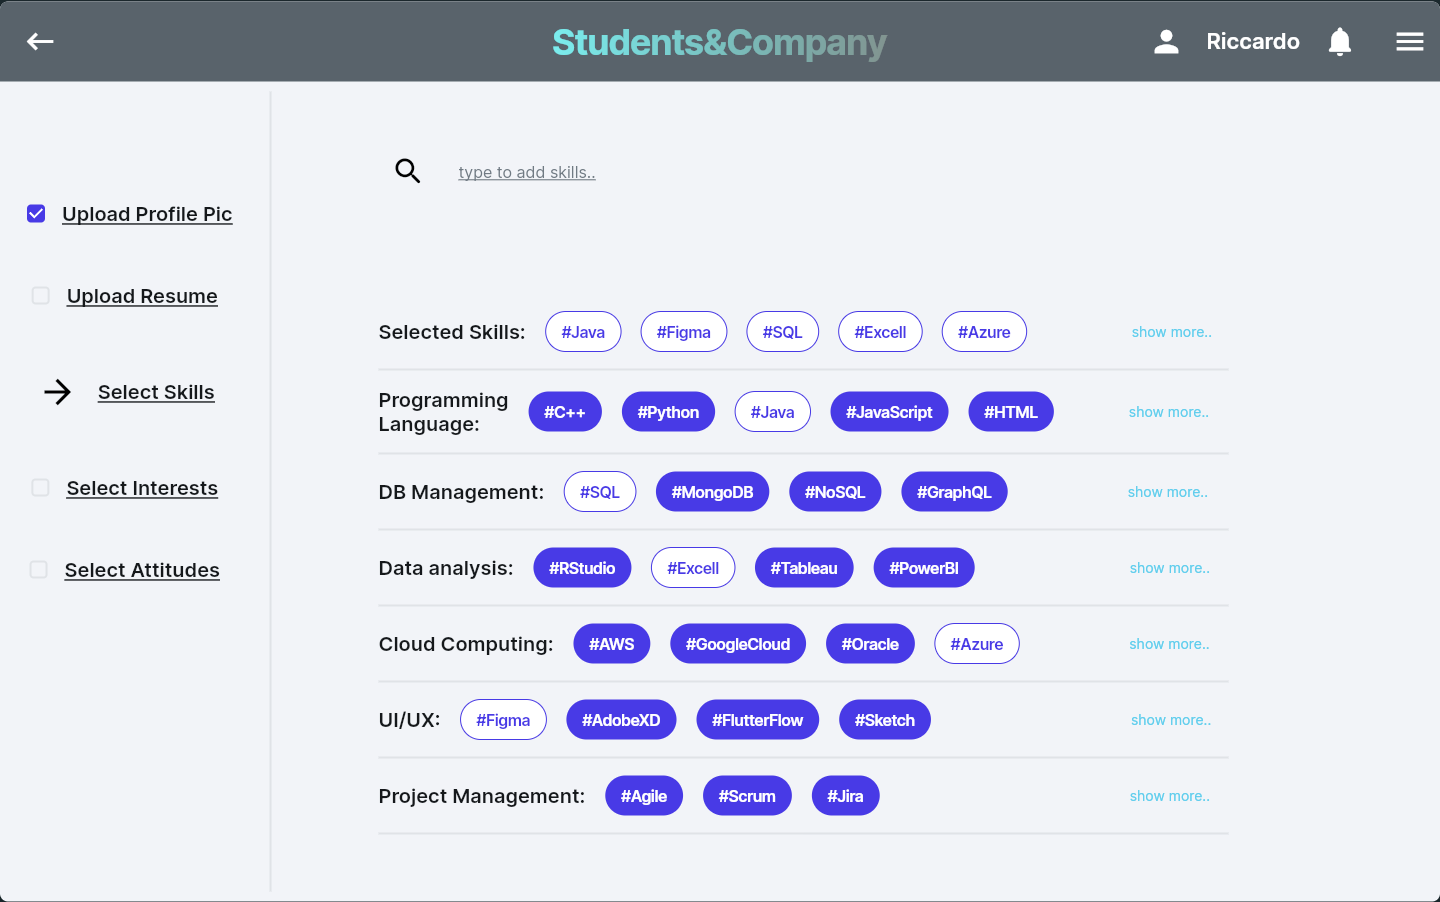
\includegraphics[width=0.7\linewidth]{Interfaces_UI/UpdateProfilePage.png}
        \caption{Update Profile Page.}
        \label{fig:update_profile_page}%
    \end{center}
\end{figure}

The "Update Profile" form page is where the STs can enrich their profile overview by setting some pre-defined parameters that best describe them. This process starts with uploading a profile picture, a resume, select the individual skills, interests and attitude, but anyone can skip any of the steps, knowing that poor profiles are less likely to be matched with the right internship.

\subsection*{UI\cui . CP Homepage}

\begin{figure}[H]
    \begin{center}
        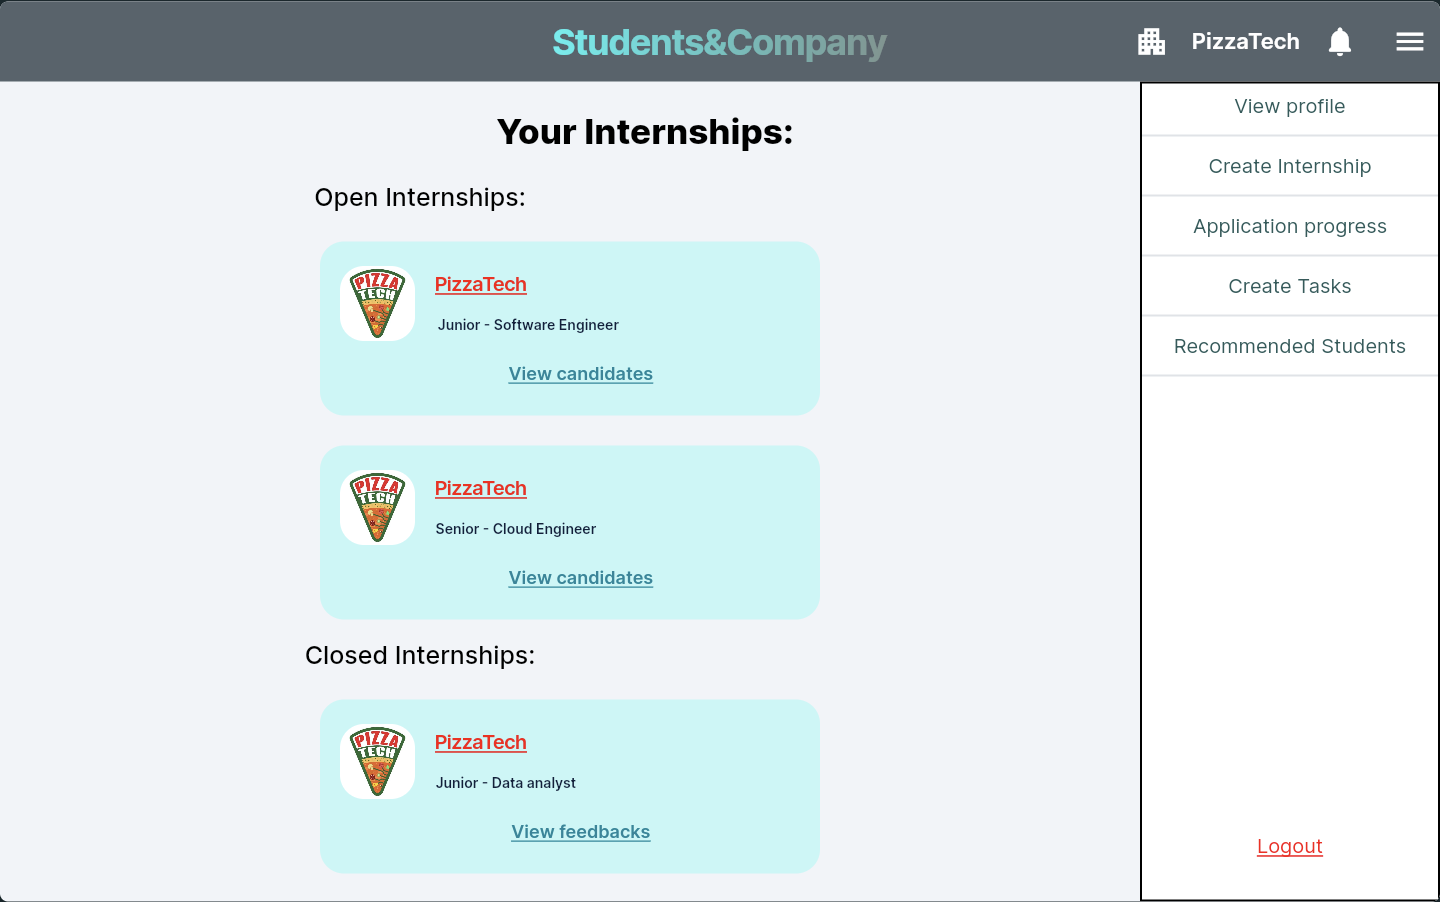
\includegraphics[width=0.7\linewidth]{Interfaces_UI/CPHomePage.png}
        \caption{CP Homepage.}
        \label{fig:company_homepage}%
    \end{center}
\end{figure}

From the Login Page, the CP will be redirected to the Company Homepage, which is composed by the published internship by them. Clicking on top of an internship redirect to the View Internship page, which provides an overview of everything the CP needs to know.

\subsection*{UI\cui . Create Internship Page}

\begin{figure}[H]
    \begin{center}
        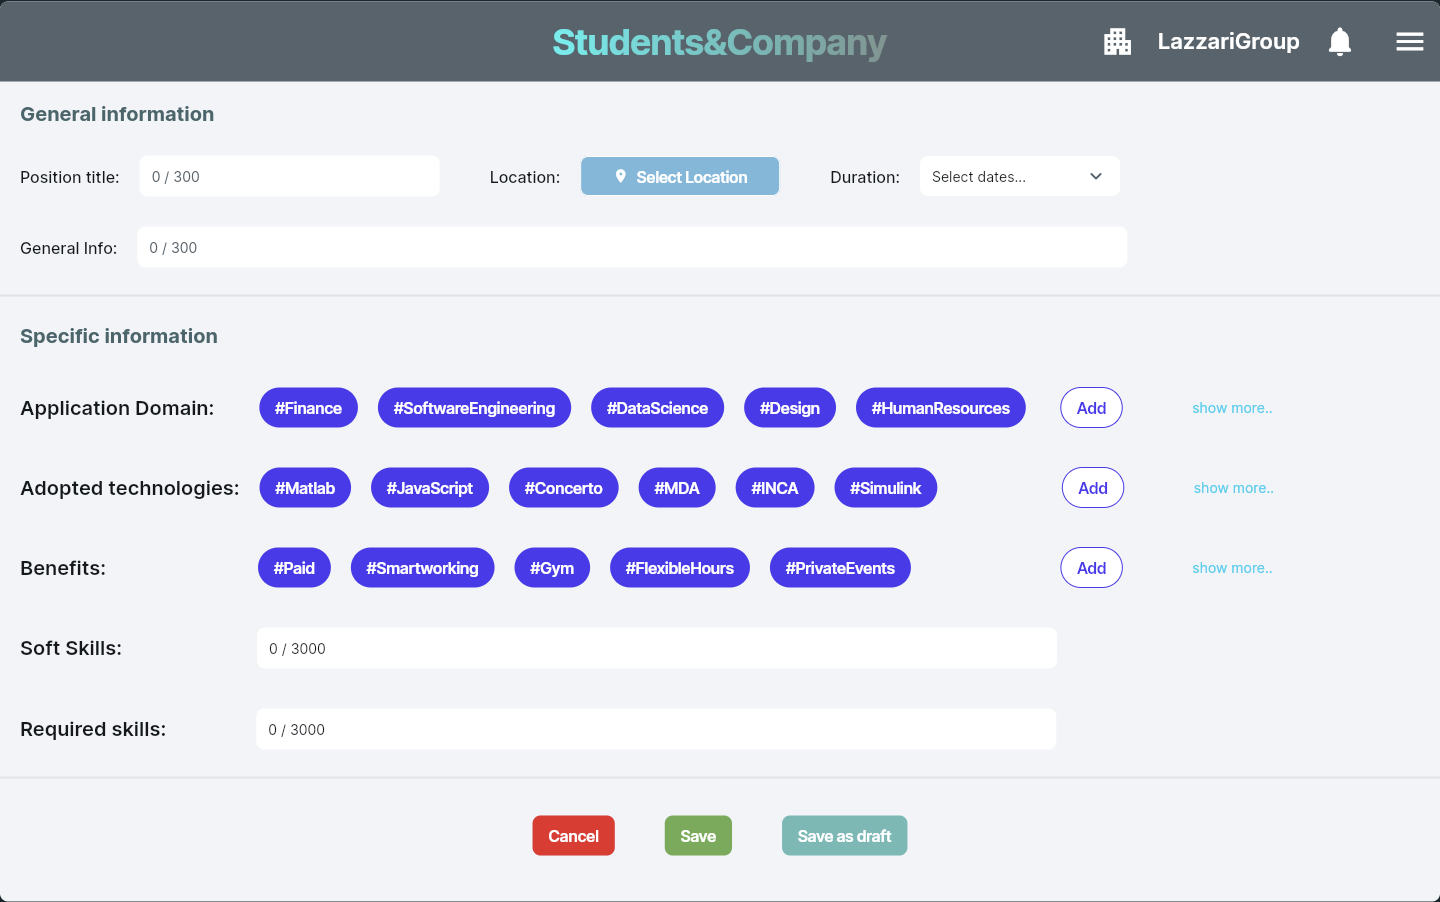
\includegraphics[width=0.7\linewidth]{Interfaces_UI/CreateInternshipPage.png}
        \caption{Create Internship Page.}
        \label{fig:create_internship_page}%
    \end{center}   
\end{figure}

In the "Create Internship" page, the CP can start to create a new announcement for an internship, starting by filling the General information forms, which include the position title, location, duration and some other general info.
After that, the CP can start filling in the specific information forms by selecting some of the predefined tags that could be inherent to the internship they're proposing. At any moment the CP can cancel, pause or publish this process by clicking on the "Cancel", "Save as Draft" or "Publish" buttons at the bottom of the page.

\subsection*{UI\cui . View Profile Page}

\begin{figure}[H]
    \begin{center}
        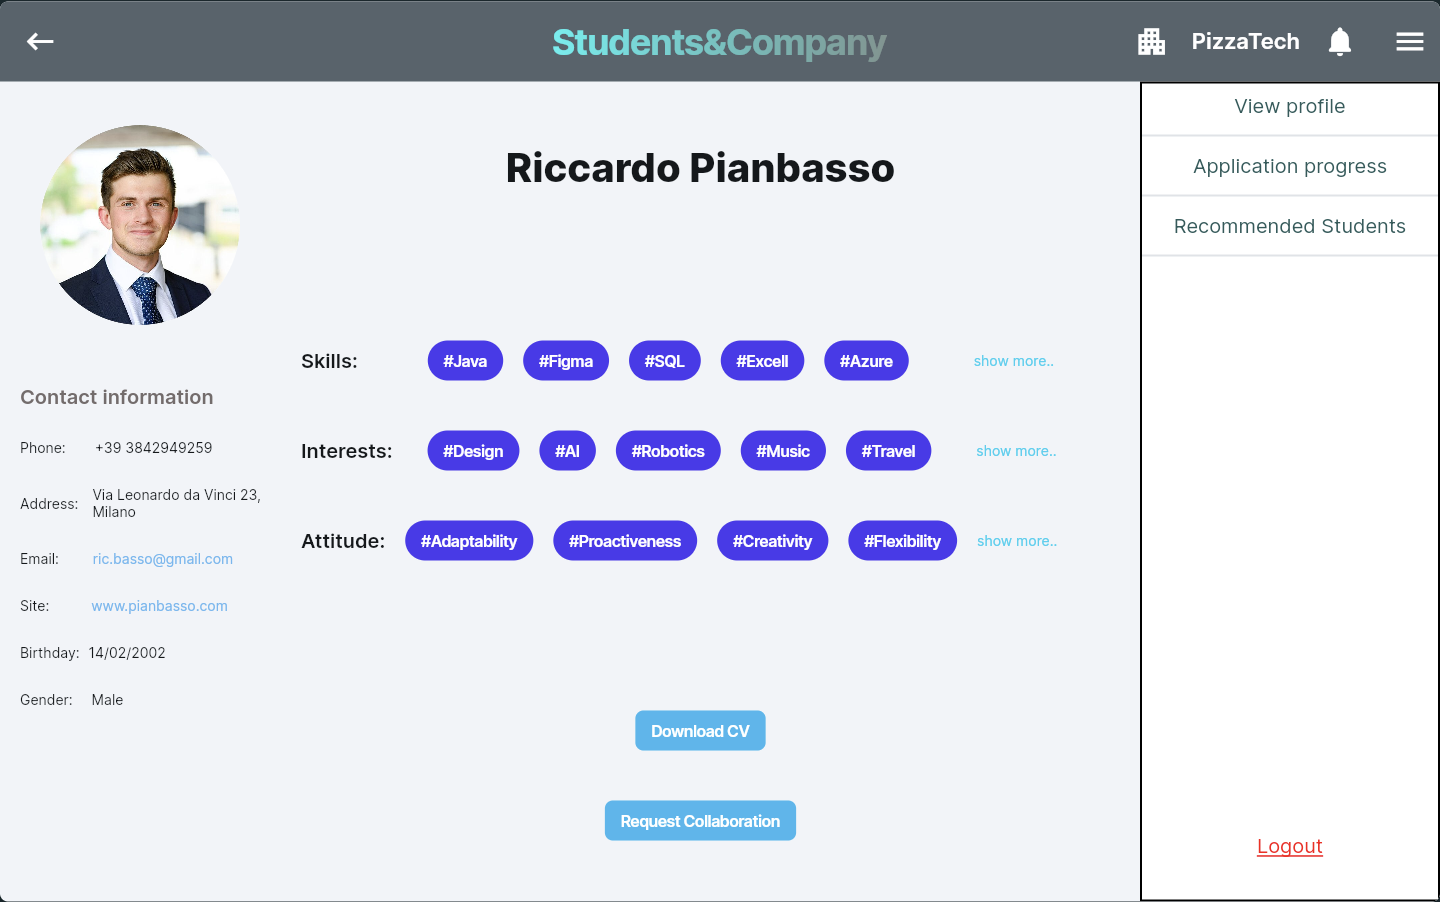
\includegraphics[width=0.7\linewidth]{Interfaces_UI/ViewProfilePage.png}
        \caption{View Profile Page.}
        \label{fig:view_profile_page}%
    \end{center}
\end{figure}

The "View Profile" page provides an overview of the student, and based on the User that is visualizing this page, some functionality may appear. In this case the company PizzaTech has received a matching notification for this student, and now has the possibility to contact him by clicking on the "Request Collaboration" button.

\subsection*{UI\cui . View Internship Page}

\begin{figure}[H]
    \begin{center}
        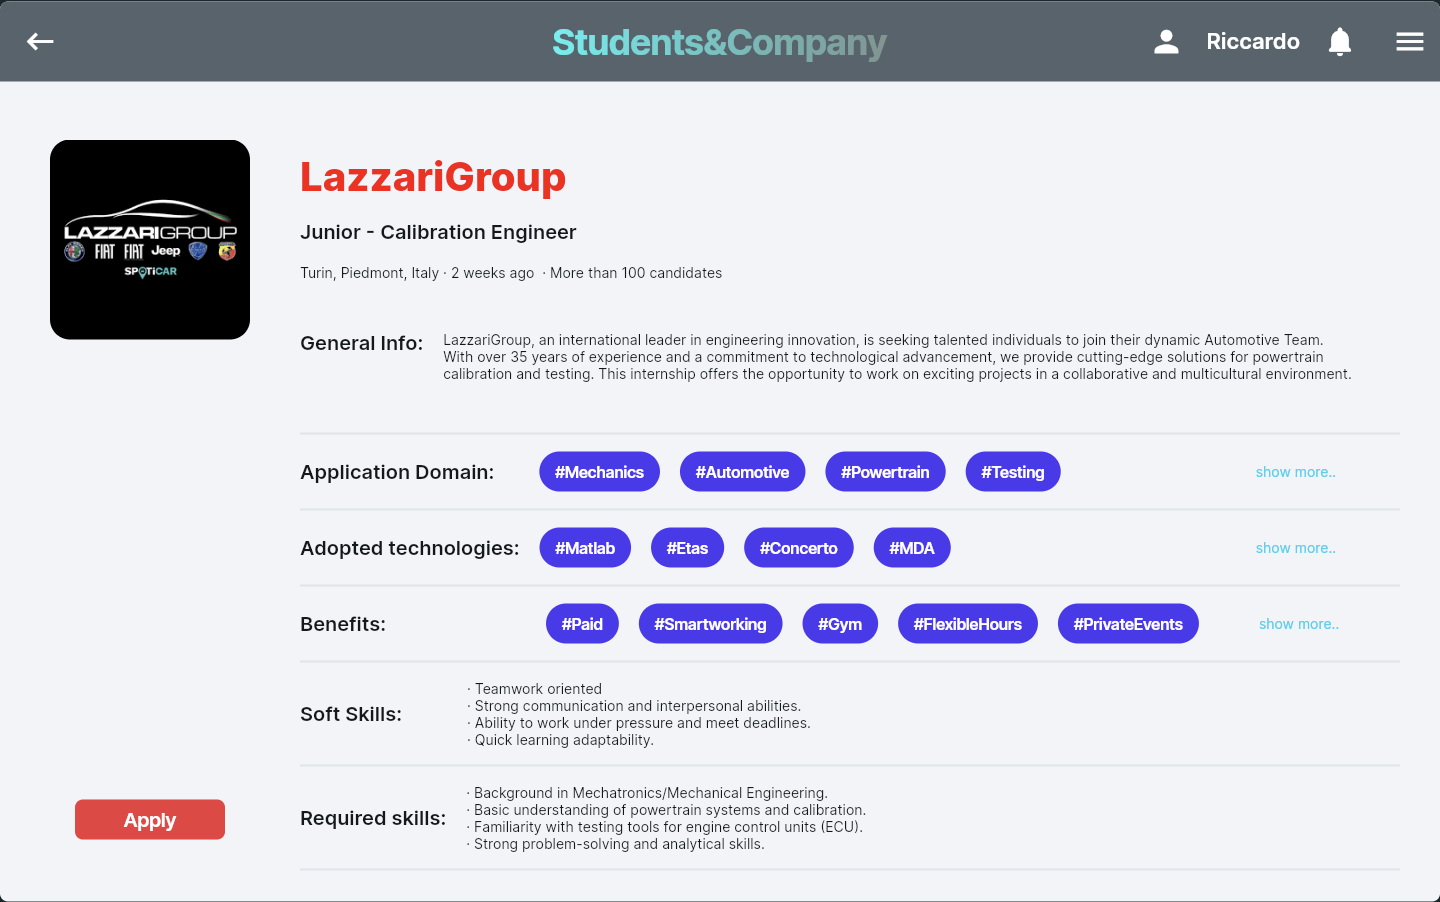
\includegraphics[width=0.7\linewidth]{Interfaces_UI/ViewInternshipPage.png}
        \caption{View Internship Page.}
        \label{fig:view_internship_page}%
    \end{center}
\end{figure}

The "View Internship" page displays all the general and specific information of an internship. Depending on the User who visualizes the page, some changes may appear, as in this case is present the "Apply" button is present, which appears when a ST views this page. In case it is the publishing company that visualizes this page, it can also modify the parameters and the status of the internship.

\subsection*{UI\cui . Application Progress Page}

\begin{figure}[H]
    \begin{center}
        \includegraphics[width=0.7\linewidth]{Interfaces_UI/applicationProgressPage.png}
        \caption{Application Progress Page.}
        \label{fig:application_progress_page}%
    \end{center}   
\end{figure}

The "Application Progress" page allows both Students (ST) and Companies (CP) to track the status of a specific internship application for a student. For a Student, this page provides a clear visualization of the progress of their internship journey, categorized into four distinct phases:

\begin{itemize}
    \item \textbf{Open}: This status represents internships that are still in the initial phase, where applications have been submitted but the selection process has not yet begun.
    \item \textbf{Selection}: In this phase, the company evaluates candidates by assigning tasks or conducting interviews to determine the most suitable applicants.
    \item \textbf{Ongoing}: This is the active phase of the internship, where the student is already working with the company.
    \item \textbf{Closed}: The final phase, marking the completion of the internship. At this stage, students can provide feedback regarding their experience.
\end{itemize}
This page provides an intuitive and structured way for users to understand the progress of each application at a glance.








    \chapter{Requirements Traceability}
    \label{ch:requirements_traceability}%
    \paragraph{LoginManager:}
\begin{itemize}
    \item R2: CKB allows registered EDs to login 
    \item R3: CKB allows registered STs to login
\end{itemize}


\paragraph{RegistrationManager:}
\begin{itemize}
    \item R1: CKB allows unregistered Users to sign up 
    \item R46: CKB shall communicate with the mailing system in order to allow Users to register their account 
\end{itemize}


\paragraph{CreateTournament:}
\begin{itemize}
    \item R4: CKB allows EDs to create Tournaments 
    \item R5: CKB allows EDs to grant the permissions of a Tournament to other EDs
    \item R15: CKB allows EDs to choose which Badges to award in a certain Tournament 
\end{itemize}


\paragraph{CreateBattle:}
\begin{itemize}
    \item R6: CKB allows EDs to create Battles 
    \item R7: CKB allows EDs to uploads the code kata of a Battle 
    \item R8: CKB allows EDs to set the minimum and the maximum number of STs per group of a Battle 
    \item R9: CKB allows EDs to set a registration deadline of a Battle 
    \item R10: CKB allows EDs to set a submission deadline of a Battle 
    \item R11: CKB allows EDs to set additional configuration for the scoring system of a Battle 
    \item R12: CKB allows EDs to set functional aspects for the scoring system of a Battle
    \item R30: CKB creates a GH repository of the code kata when the registration deadline for the Battle expires 
    \item R31: CKB sends the link of the GH repository to every STG that participates in the Battle 
\end{itemize}


\paragraph{CreateGroup:}
\begin{itemize}
    \item R22: CKB allows STs to create a new STG 
    \item R23: CKB allows STs to join a STG 
    \item R24: CKB allows STs to invite other STs in their STG
\end{itemize}


\paragraph{OpenProfile:}
\begin{itemize}
    \item R18: CKB allows EDs to visualize the profile of another User 
    \item R19: CKB allows STs to visualize the profile of another User
\end{itemize}


\paragraph{JoinTournament:}
\begin{itemize}
    \item R20: CKB allows STs to join a Tournament 
\end{itemize}


\paragraph{ViewTournament:}
\begin{itemize}
    \item R41: CKB allows STs to check the Leaderboard of a Tournament 
    \item R42: CKB allows EDs to check the Leaderboard of a Tournament
\end{itemize}


\paragraph{CloseTournament:}
\begin{itemize}
    \item R17: CKB allows EDs to close a Tournament 
    \item R49: CKB shall assign the Badges to all STs that fulfill their requirements 
\end{itemize}


\paragraph{CreateBadge:}
\begin{itemize}
    \item R13: CKB allows EDs to create new Badges 
\end{itemize}


\paragraph{ModifyBadge:}
\begin{itemize}
    \item R14: CKB allows EDs to choose the rules related to the awarding of Badges 
\end{itemize}


\paragraph{JoinBattle:}
\begin{itemize}
    \item R21: CKB allows STs to join a Battle 
    \item R47: STs need to fork the GH repository of the Battle they are participating in 
\end{itemize}


\paragraph{ViewBattle:}
\begin{itemize}
    \item R35: CKB allows STs to check the Leaderboard of a Battle 
    \item R36: CKB allows EDs to check the Leaderboard of a Battle
\end{itemize}


\paragraph{EndBattle:}
\begin{itemize}
    \item R16: CKB allows EDs to assign a score manually during the consolidation stage 
\end{itemize}


\paragraph{ManualEvaluation:}
\begin{itemize}
    \item R16: CKB allows EDs to assign a score manually during the consolidation stage 
    \item R37: CKB allows EDs to analyze the code of a STG 
\end{itemize}


\paragraph{AutomatedEvaluation:}
\begin{itemize}
    \item R32: CKB evaluates the STG's work every time a push is made on GH and calculates Battle score for the STG 
    \item R33: CKB updates the Battle Leaderboard once a new score is registered 
    \item R34: CKB updates the Tournament Leaderboard once a new score is registered
    \item R44: CKB shall communicate with the GH API in order to calculate a new score every time a push action is made by a STG 
    \item R45: CKB shall communicate with the external tool in order to calculate the score of a STG
\end{itemize}


\paragraph{Model:}
\begin{itemize}
    \item R25: CKB stores the informations about the Users 
    \item R26: CKB shall ensure security of data
\end{itemize}


\paragraph{DashBoardManager:}
\begin{itemize}
    \item R39: CKB allows STs to check the list of ongoing Tournaments 
    \item R40: CKB allows EDs to check the list of ongoing Tournaments
\end{itemize}


\paragraph{NotificationManager:}
\begin{itemize}
    \item R27: CKB sends notifications to every ST when a new Tournament is created 
    \item R28: CKB sends notifications when a new Battle is created to every ST which is participating in the Tournament that the Battle is part of
    \item R29: CKB sends notifications to a ST when he receives an invitation to be part of STG
    \item R38: CKB sends notifications to every STs participating in the Battle once the consolidation stage ends
    \item R43: CKB sends notifications to every ST involved in a Tournament when the Tournament is closed and the final ranks are available
    \item R50: CKB sends notifications to the ED when he receives the permission to create Battles in a Tournament

\end{itemize}




    \chapter{Implementation, Integration and Test Plan}
    \label{ch:Implementation_integration_test_plan}%
    \section{Overview and Implementation Plan}

In this last chapter, it will be described the Implementation of the system, the Integration and the Test Strategy that has to be followed. In general, the method that will be followed is a Bottom-Up strategy.\\
By adopting this strategy, the implementation will start from the leaves of the ‘uses’ hierarchy, starting from the small functionalities that do not require other functionalities to work. These modules will require a Driver each that will be developed in order to be tested. Once a new module is developed and tested, it may be integrated into the system and replace a previously existing Driver, but the new module will require a new Driver in order to be tested. In this way several working subsystems are created, which will be eventually integrated into the final one. Bottom-Up strategy promotes an incremental integration, that makes it easier to track bugs and errors, given that the testing is going to be done on a reduced part of the system at the beginning and on every module once it is ready. This strategy also allows independent development teams to work in parallel on different functions.


\section{Features Identification}

\paragraph{[F1] Login and Registration Features.} These are the basic features of CKB, that will be needed by every User, both Educators and Students. Though this set of features will require the least amount of time to be implemented, its role will be crucial to the proper functioning of the entire Web App. Since they are required for the correct workflow of the following features, they will also be the first to be implemented.

\paragraph{[F2] Creation Features.} This set of features includes every creation feature, such as the creation of Tournaments, Battles, Groups or Badge, whatever represents the creation of a new Bean or a write operation on the database. These features are required for the following features, since without them it wouldn’t be possible to visualize a Battle or Tournament.

\paragraph{[F3] View Features.} These features include the possibility to open the page of a Tournament, a Battle, a User Profile, or the Home Page. They need the correspondent \textbf{F2} feature in order to work and are essential for the Search and Join Features.

\paragraph{[F4] Search Features.} These features include the use of the search bar on the website in order to retrieve the list of the ongoing Tournaments, Battles or Users. These features require that \textbf{F2} and \textbf{F3} are implemented but aren’t needed by other features.

\paragraph{[F5] Join Features.} Include the operations that permit joining a Tournament, a Battle, or a Group. This set of features need the view and creation features to exist, before getting implemented.

\paragraph{[F6] Evaluation Features.} Features that include Manual and Automated Evaluation using the External Tools. 

\paragraph{[F7] Notification Features.} This is the last possible set of features to be developed, since the proper functioning of this feature requires that every other kind of feature properly functions too.  

\newpage
\section{Integration Strategy}
The integration of components and the testing of the system should start as soon as the DBMS and the host server are ready. The connections with the Mailing System, GitHub and the External Tools are not required since the starting moment, but will be necessary once the corresponding features will be integrated. As explained before the integration will follow a bottom-up approach.
\\
Starting from the model, which will be tested alongside a proper driver, 


\begin{figure}[H]
    \begin{center}
        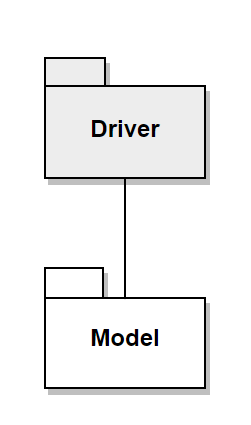
\includegraphics[width=0.2\linewidth]{Integration/I1.png}
        \label{fig:Integration_1}%
    \end{center}
\end{figure}


The integration of components will proceed with the Login and Registration features:

\begin{figure}[H]
    \begin{center}
        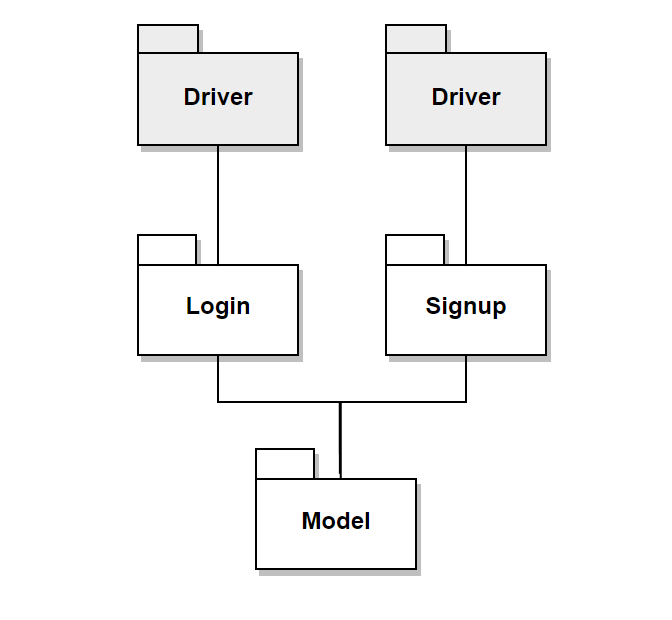
\includegraphics[width=0.4\linewidth]{Integration/I2.png}
        \label{fig:Integration_2}%
    \end{center}
\end{figure}

Once they will be developed and tested, it will be the turn of the components that perform a creation feature and their drivers:

\begin{figure}[H]
    \begin{center}
        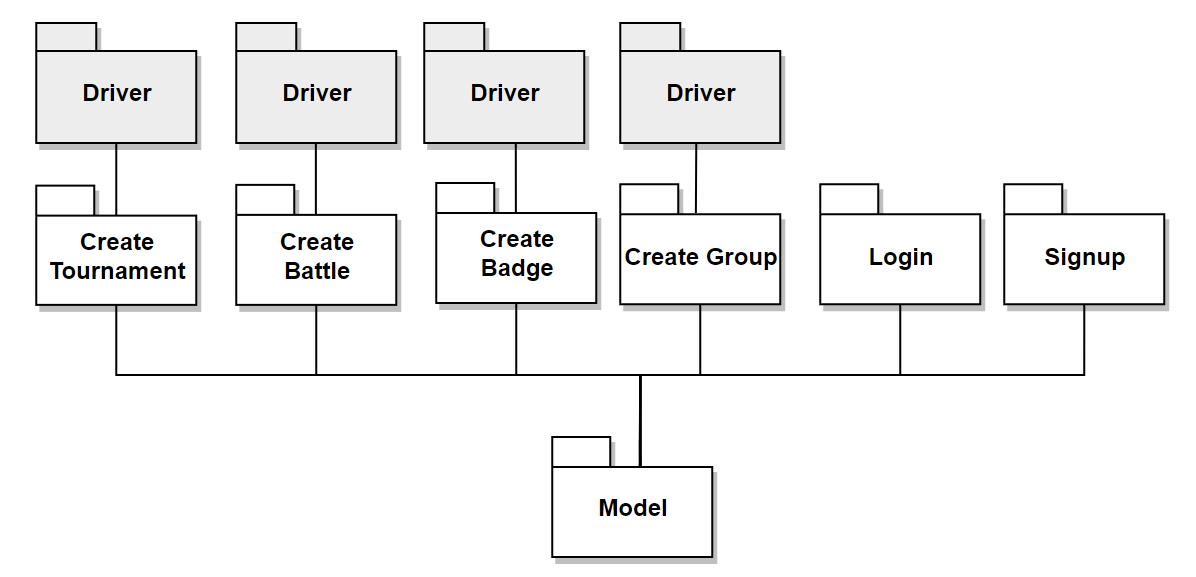
\includegraphics[width=0.8\linewidth]{Integration/I3.png}
        \label{fig:Integration_3}%
    \end{center}
\end{figure}

Now it is possible to create Tournaments, Battles, Groups and Badges functions to view those elements’ pages or the search components can be integrated.


\begin{figure}[H]
    \begin{center}
        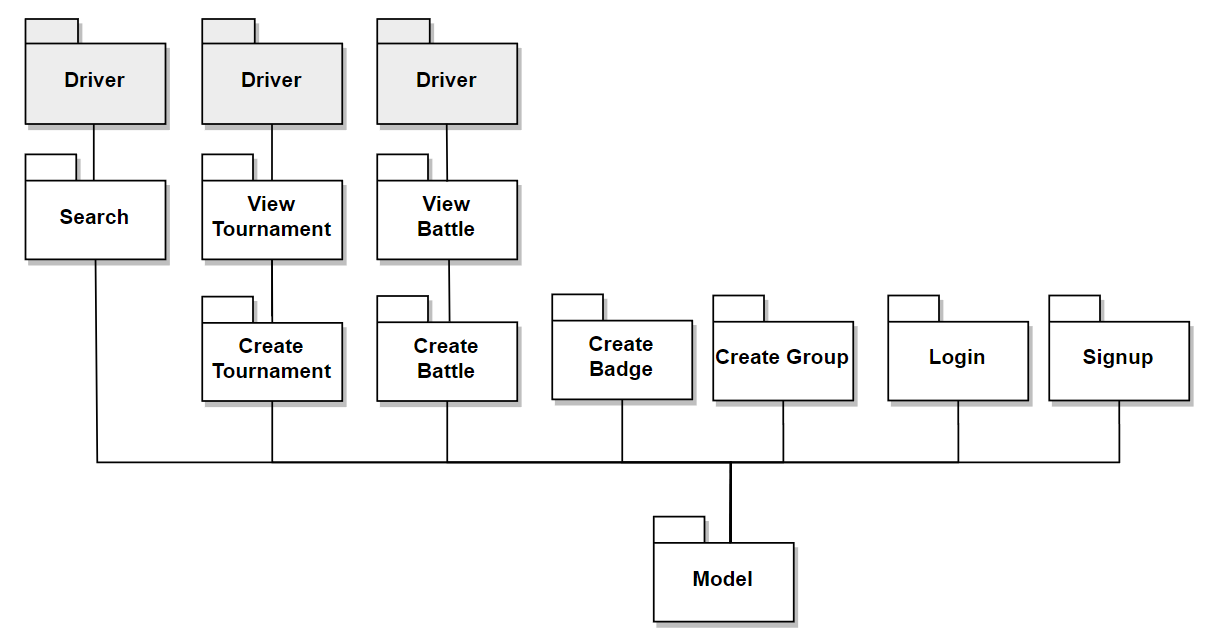
\includegraphics[width=0.8\linewidth]{Integration/I4.png}
        \label{fig:Integration_4}%
    \end{center}
\end{figure}

The last missing components in the context of Tournaments and Battles are the Join features, which will be integrated in parallel with the possibility to open Users’ profiles and to modify Badges parameters for the EDs.


\begin{figure}[H]
    \begin{center}
        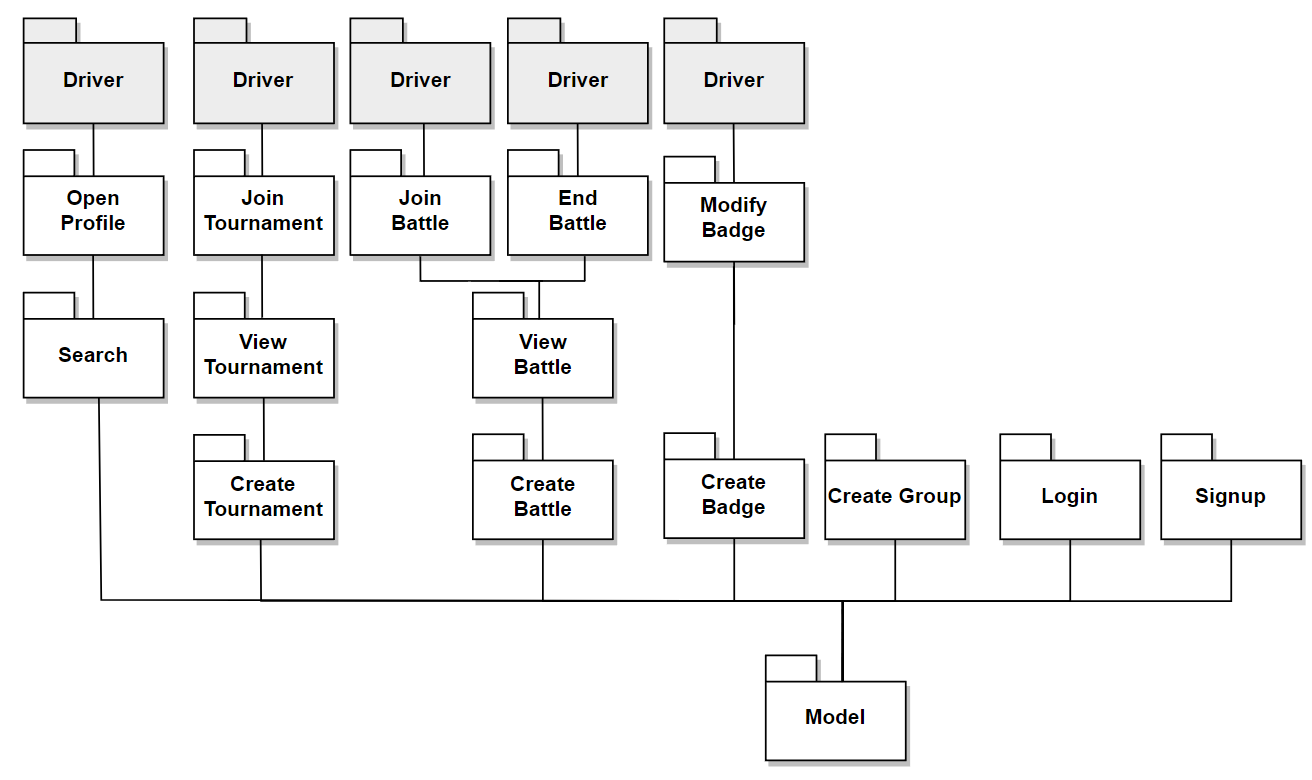
\includegraphics[width=0.8\linewidth]{Integration/I5.png}
        \label{fig:Integration_5}%
    \end{center}
\end{figure}

For the sake of simplicity, the previously integrated components are represented grouped in their Manager component (let the ‘Tournament Manager’ contain every Tournament-related component, and so on). Evaluation features will come next.

\begin{figure}[H]
    \begin{center}
        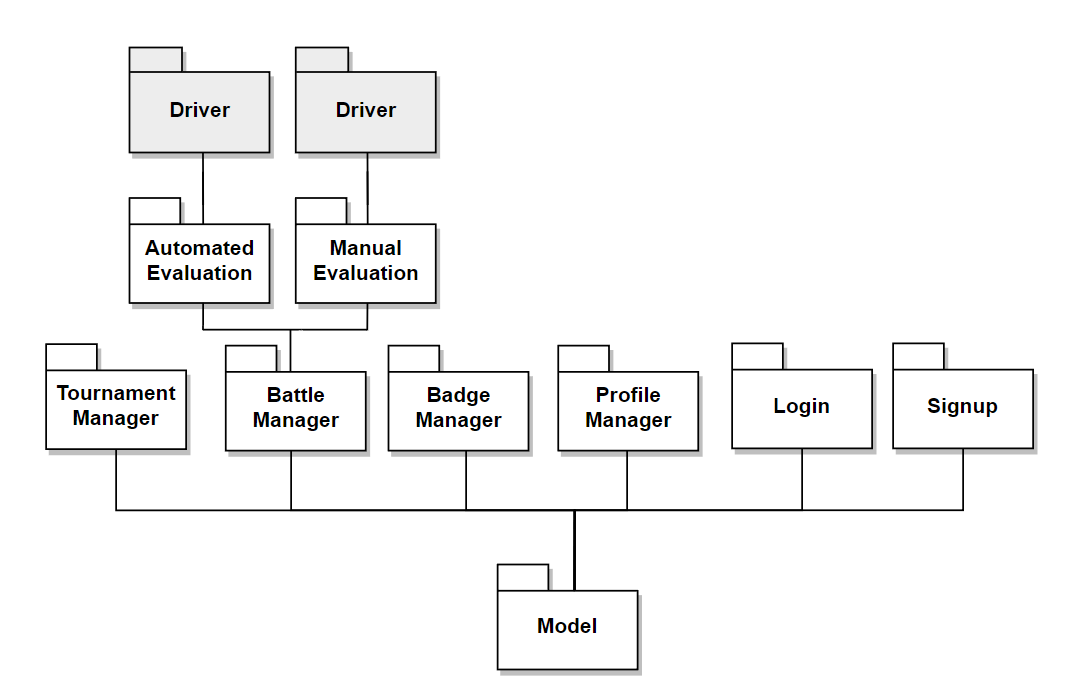
\includegraphics[width=0.8\linewidth]{Integration/I6.png}
        \label{fig:Integration_6}%
    \end{center}
\end{figure}

Once the Evaluation features are integrated, they will be considered as the same in the ‘Evaluation Manager’. Then Notification Manager will be the next to be integrated and tested.


\begin{figure}[H]
    \begin{center}
        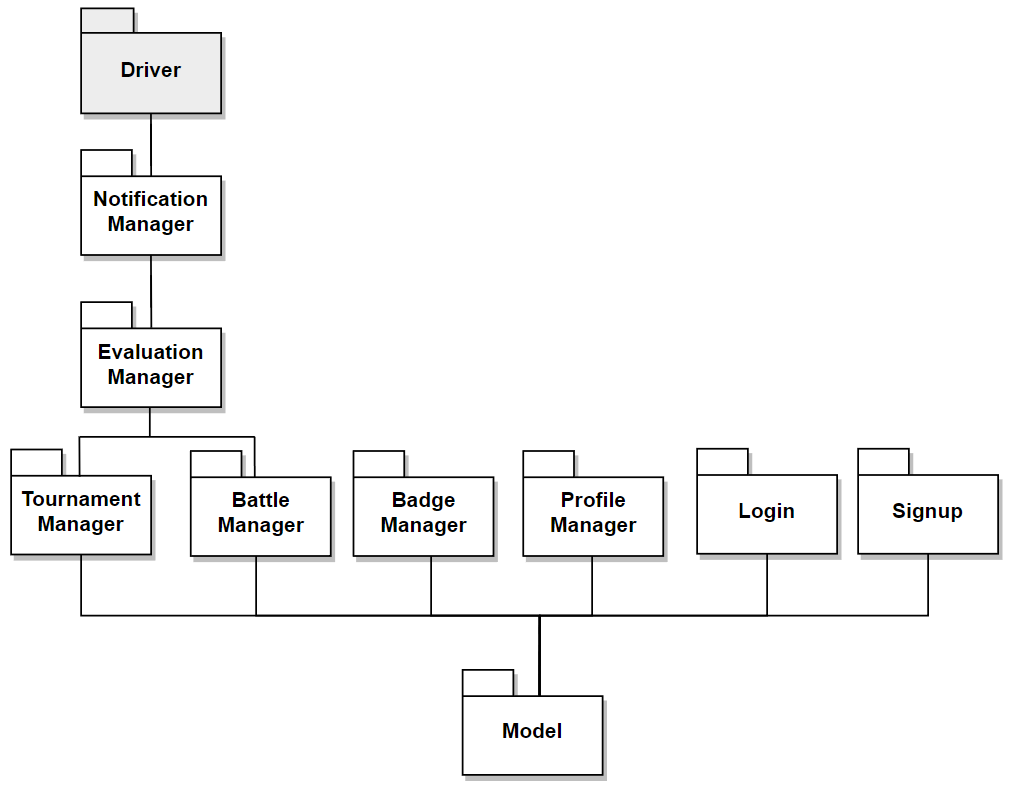
\includegraphics[width=0.8\linewidth]{Integration/I7.png}
        \label{fig:Integration_7}%
    \end{center}
\end{figure}

The last component that has to be integrated is the dashboard Manager, that is essential for the correct workflow of the user interface.


\begin{figure}[H]
    \begin{center}
        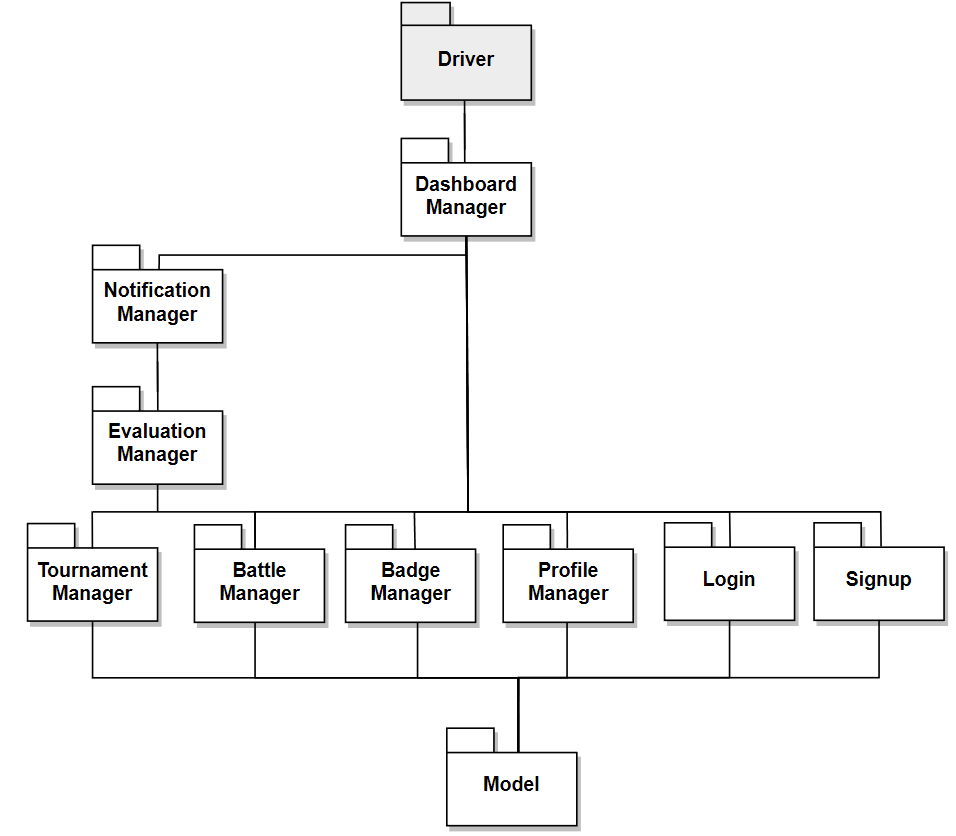
\includegraphics[width=0.8\linewidth]{Integration/I8.png}
        \label{fig:Integration_8}%
    \end{center}
\end{figure}

After the removal of the Dashboard Manager’s Driver, the final system is as follows.

\begin{figure}[H]
    \begin{center}
        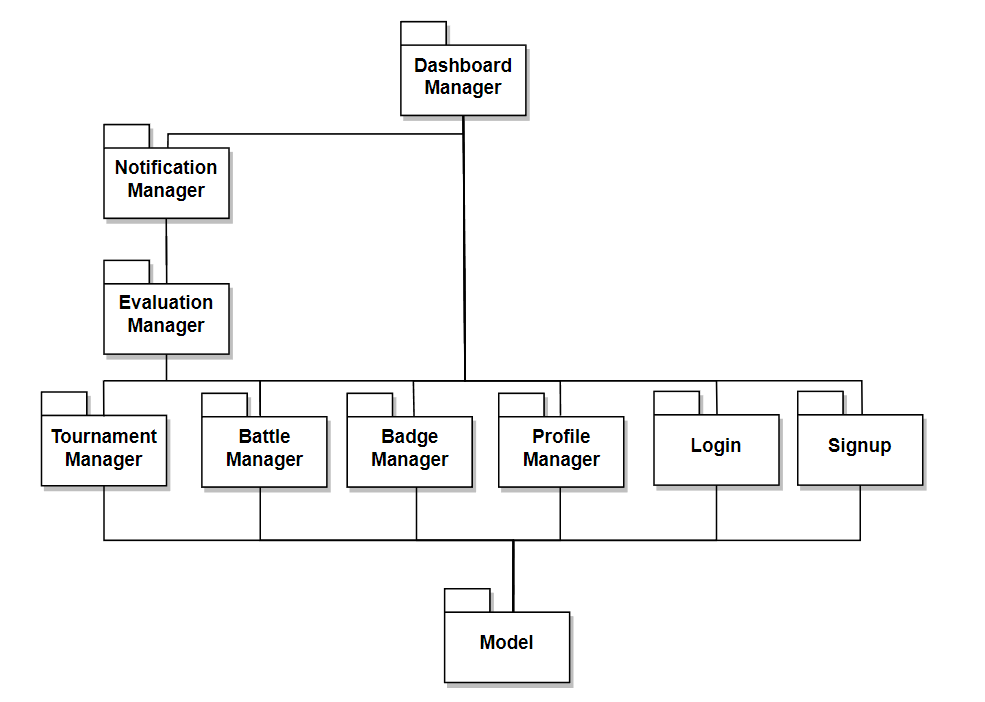
\includegraphics[width=0.8\linewidth]{Integration/IFinal.png}
        \label{fig:Integration_final}%
    \end{center}
\end{figure}



\section{System Testing Strategy}

It is necessary to check that each newly developed component works properly before integrating it with the system by the use of Drivers. Once a new component is integrated to the system, it must be checked with a new Driver that the new component is properly integrated, that the modules’ properties still hold and that the integrated system follows the correct workflow. 
Once every component is integrated, it will be needed to test the system as a whole to ensure the proper workflow is followed and the absence of bugs. In order to do so the following kinds of testing will be applied. 

\begin{itemize}
    \item \textbf{Functional Testing: }Functional Testing will be performed on the system to guarantee that the workflow is correct and consistent with the functionalities described in the RASD document, checking the fulfillment of goals, requirements and use cases and the possibility to correctly simulate the described scenarios. 
    \item \textbf{Load Testing:} Load Testing is useful in order to find eventual memory leaks, buffer overflows and bad management of memory.
    \item \textbf{Performance Testing:} The system will undergo this kind of testing in order to identify bottlenecks and to observe the resilience of the system under heavy workload, keeping in mind that the system shall support many users working simultaneously keeping response times as low as possible, following what is stated in the \textit{RASD document, section 3.3}. This will also help to identify optimization possibilities in the software’s algorithms.
    \item \textbf{Stress Testing:} In order to make sure that the system is capable of recovering itself after a failure, Stress Testing will be adopted, by simulating lots of concurrent users or reducing the system’s computational resources.
    \item \textbf{User Interface Testing:} It is important that the system correctly works on different kinds of devices, and different browsers as stated during the Requirements Analysis, testing the usability and accessibility of the web app on every possible platform, for both kinds of users: EDs and STs. 
\end{itemize}


    \chapter{Effort Spent}
    \label{ch:effort_spent}%
    \begin{table}[H]
    \begin{center}
        \begin{tabular}{c|c}
            \hline
            Member of group & Effort spent \\
            \hline
            Pianalto Riccardo & \begin{tabular}{p{0.5\linewidth}|c}
                             Introduction          & $??h$  \\
                             Architectural Design   & $??h$ \\
                             User Interface Design & $??h$ \\
                             Requirements Traceability       & $??h$ \\
                             Implementation Integration Test Plan & $??h$ \\
            \end{tabular} \\
            \hline
            Pica Mirko & \begin{tabular}{p{0.5\linewidth}|c}
                             Introduction          & $??h$  \\
                             Architectural Design   & $??h$ \\
                             User Interface Design & $??h$ \\
                             Requirements Traceability & $??h$  \\
                             Implementation Integration Test Plan & $??h$ \\
            \end{tabular} \\
            \hline
            Prendin Christian & \begin{tabular}{p{0.5\linewidth}|c}
                                     Introduction          & $2h$ \\
                                     Architectural Design   & $20h$ \\
                                     User Interface Design & $15h$ \\
                                     Requirements Traceability & $0.5h$ \\
                                     Implementation Integration Test Plan & $1h$ \\
            \end{tabular} \\
            \hline
        \end{tabular}
        \caption{Effort spent by each member of the group.}
        \label{tab:effor_spent}
    \end{center}
\end{table}





    \chapter{References}
    \label{ch:references}%
    \section{References}
\label{sec:references}%

\begin{itemize}
    \item ISO/IEC/IEEE29148:2018 - Systems and software engineering - Life cycle processes - Requirements engineering.
    \item The Requirement Engineering and Design Project specification document A.Y. 2024–2025. 
\end{itemize}

\section{Used Tools}
\label{sec:used_tools}%
\begin{itemize}
    \item \textit{GitHub} for project versioning and sharing.
    \item \LaTeX{} and \textit{Overleaf} as editor for writing this document.
    \item \textit{sequencediagram.org} for the sequence diagrams' design.
    \item \textit{Lucidchart} and \textit{draw.io} for the other diagrams' design.
    \item \textit{FlutterFlow} for the User Interface Design.
    \item \textit{Google Docs} for collaborative writing, notes and reasoning.
\end{itemize}


% LIST OF FIGURES
    \listoffigures

% LIST OF TABLES
    \listoftables
    \cleardoublepage


\end{document}